
%%%%%%%%%%%%%%%%%%%%%%% file template.tex %%%%%%%%%%%%%%%%%%%%%%%%%
%
% This is a general template file for the LaTeX package SVJour3
% for Springer journals.          Springer Heidelberg 2010/09/16
%
% Copy it to a new file with a new name and use it as the basis
% for your article. Delete % signs as needed.
%
% This template includes a few options for different layouts and
% content for various journals. Please consult a previous issue of
% your journal as needed.
%
%%%%%%%%%%%%%%%%%%%%%%%%%%%%%%%%%%%%%%%%%%%%%%%%%%%%%%%%%%%%%%%%%%%
%
% First comes an example EPS file -- just ignore it and
% proceed on the \documentclass line
% your LaTeX will extract the file if required
\begin{filecontents*}{example.eps}
%!PS-Adobe-3.0 EPSF-3.0
%%BoundingBox: 19 19 221 221
%%CreationDate: Mon Sep 29 1997
%%Creator: programmed by hand (JK)
%%EndComments
gsave
newpath
  20 20 moveto
  20 220 lineto
  220 220 lineto
  220 20 lineto
closepath
2 setlinewidth
gsave
  .4 setgray fill
grestore
stroke
grestore
\end{filecontents*}
%
\RequirePackage{fix-cm}
%
\documentclass{svjour3}                     % onecolumn (standard format)
%\documentclass[smallcondensed]{svjour3}     % onecolumn (ditto)
%\documentclass[smallextended]{svjour3}       % onecolumn (second format)
%\documentclass[twocolumn]{svjour3}          % twocolumn
%
\smartqed  % flush right qed marks, e.g. at end of proof
%
\usepackage{graphicx}
\usepackage{caption}    
\usepackage{subfig} 
\usepackage{todonotes}
%
% \usepackage{mathptmx}      % use Times fonts if available on your TeX system
%
% insert here the call for the packages your document requires
%\usepackage{latexsym}
% etc.
%
% please place your own definitions here and don't use \def but
% \newcommand{}{}
%
% Insert the name of "your journal" with
% \journalname{myjournal}
%
\begin{document}

\title{The Pandora multi-algorithm approach to automated pattern recognition of cosmic-ray muon and test beam particle interactions in the ProtoDUNE-SP detector
%\thanks{Grants or other notes
%about the article that should go on the front page should be
%placed here. General acknowledgments should be placed at the end of the article.}
}
%\subtitle{Do you have a subtitle?\\ If so, write it here}

\author{S. Green \and
        J. Marshall \and 
        L. Escudero Sanchez \and 
        A. Blake
}

\titlerunning{The Pandora Reconstruction for ProtoDUNE-SP}
%\authorrunning{Short form of author list} % if too long for running head

\institute{S. Green \at
            University of Cambridge, Cambridge, CB3 0HE, United Kingdom
%           \emph{Present address:} of F. Author  %  if needed
            \and
            J. Marshall \at
            University of Warwick
            \and 
            L. Escudero Sanchez \at
            University of Cambridge, Cambridge, CB3 0HE, United Kingdom
            \and 
            A. Blake \at 
            University of Lancaster
}

\date{Received: date / Accepted: date}
% The correct dates will be entered by the editor

\maketitle

\begin{abstract}
Pattern recognition is an essential aspect of event reconstruction at Liquid-Argon Time-Porjection Chamber detectors.  The Pandora software package has been developed and successfully applied to several ongoing neutrino LArTPC detector experiments.  Now Pandora is being applied to ProtoDUNE-SP, a test beam experiment prototyping detector technologies for use at the DUNE far detector.  The Pandora multi-algorithm approach to pattern recognition enables complex, high energy test beam particle interaction topologies to be reconstructed successfully and the interaction hierarchy determined.  This paper gives an overview of the Pandora reconstruction algorithms used for ProtoDUNE-SP and evaluates the performance for both simulation and data.
\keywords{Pattern recognition \and Event reconstruction \and Neutrino detectors \and Time-projection chambers \and DUNE \and ProtoDUNE-SP}
% \PACS{PACS code1 \and PACS code2 \and more}
% \subclass{MSC code1 \and MSC code2 \and more}
\end{abstract}

\section{Introduction}
\label{sec:intro}
ProtoDUNE-SP is a single phase liquid argon time projection chamber (LArTPC) detector prototype for the DUNE far detector.  It was completed and began taking data in late 2018, recording test beam data at CERNs Neutrino Platform from October to the start of the long shutdown in December.  The detector is continuing to take cosmic ray data during the shutdown.  

The primary engineering goal of the ProtoDUNE-SP detector is to prototype the production of large scale TPCs for use at the DUNE far detector.  Alongside refinement of production procedures, ProtoDUNE-SP has several physics goals related to testing the reconstruction and performing detector calibration in a controlled environment.  Furthermore, measurements of the cross-section for various test beam particle species on a liquid argon target will be crucial for modeling neutrino interactions at the DUNE far detector.

Pandora is a software package that has been developed for event reconstruction in high energy physics and is now in use at ProtoDUNE-SP.  It consists of a framework, the Pandora Software Development Kit (SDK) \cite{pandorasdk}, and a number of different, experiment specific, content libraries containing the pattern recognition logic.  Although originally developed for event reconstruction at future linear $\text{e}^{+}\text{e}^{-}$ colliders, Pandora has been successfully applied for event reconstruction at LArTPC experiments including the MicroBooNE experiment \cite{pandorauboone}.  Pandora brings a multi-algorithm philosophy to event reconstruction, whereby algorithms are sequentially applied to build up the reconstruction from the raw inputs.  Each algorithm is designed to be simple and conservative in order to not introduce errors that would require resolving by subsequent algorithms.  Pandora now also incorporates machine learning techniques, such as Boosted Decision Trees (BDTs) and support vector machines, to drive key decisions that have to be made at certain junctions of the reconstruction. 

The Pandora reconstruction algorithms used at ProtoDUNE-SP mirror those used at MicroBooNE, which are extensively described in \cite{pandorauboone}.  Therefore, the aim of this paper is to give an overview of thsoe algorithms, highlighting specific ProtoDUNE-SP related developments, and to evaluate the performance of Pandora for both ProtoDUNE-SP simulation and data.  Section \ref{sec:protodunesp} describes the ProtoDUNE-SP detector and section \ref{sec:patrec} described the Pandora reconstruction.  Section \ref{sec:assesmentpatrec} demonstrate an assessment of the pattern performance for both ProtoDUNE-SP simulation and data.  

%-Abstract and introduction, covering Pandora background, its use across LArTPC programme, ProtoDUNE and aspects of the pattern recognition problem specific to ProtoDUNE.
%-ProtoDUNE details.
%-Pattern recognition. We?d reference the MicroBooNE algorithm description, give an executive summary of PandoraCosmic and explain how PandoraTestBeam differs from PandoraNu. In the MicroBooNE paper, we used a two-pass reconstruction, but explicitly said that this would become more sophisticated soon. This then allows us to explain the consolidated reconstruction properly, making this a major communication goal of the paper. Includes stitching, more on slicing, beam particle id.
%-Performance assessment, using MC and metrics consistent with MicroBooNE paper to assess quality of pattern recognition, understand contributions to efficiency, etc., but then moving into real data plots. Inclusion of all of the latest and greatest plots, with (ideally!) explanation of the key features.
%-Concluding comments (short).

\section{ProtoDUNE-SP}
\label{sec:protodunesp}
The ProtoDUNE-SP detector is a single phase liquid argon time projection chamber that is extensively described in \cite{pdtdr}.  Only the experiment details related to the pattern recognition side of the reconstruction are discussed in the following section.

The detector is a single-phase LArTPC with a rectangular cuboid geometry with the following dimensions: 7.4~m (horizontal), 6.0~m (vertical) and 7.0~m (longitudinal).  The ProtoDUNE-SP detector has a total volume of 0.77~kt making it the largest monolithic single phase LArTPC constructed to date.  The cryostat capacity required to accommodate that mass of argon is ~580~$\text{m}^{3}$.  The nominal electric field in the active volume is 500~V/cm.  This is provided by the Cathode Plane Assembly (CPA), which is held at -180~kV, while the Anode Plane Assemblies (APAs) is effectively grounded due to the presence of a field cage.  The anode plane assembly houses three planes of wires, two induction, hereby referred to as the \textit{u} and \textit{v} views, and one collection, the \textit{w} view.  The pitch of \textit{u} and \textit{v} views is 4.669~mm, while the pitch of the \textit{w} view is 4.790~mm.  The test beam itself is aligned parallel to the APA plane.  The \textit{u} and \textit{v} wire planes are aligned at $\pm 35.7^{0}$ to the vertical, while the \textit{w} plane wires are vertical.  

Each wire plane measures the drift time, relative to the trigger offset, of any induced or collected charge signals.  Hits are then formed from the waveforms produced from each wire by fitting the waveforms with a Gaussian.  Prior to the fitting, various detector effects are removed to reduce the background noise.  

As ProtoDUNE-SP is a surface detector, a crucial pattern recognition goal is to distinguish the cosmic ray backgrounds from the test beam particle signal.  Several other factors also affect the pattern recognition including noise filtering, fitting of the waveform and deconvolution of hit charge deposited on adjacent wires.  

\todo{Reference for noise filtering etc...}

\section{Pattern Recognition}
\label{sec:patrec}
In order to fully exploit the imaging capabilities of LArTPCs for particle physics, a paradigm shift in the field of reconstruction is required.  The detailed images of interactions LArTPCs produce make it possible to track individual particles throughout the detector and to build up a hierarchy describing their interactions.  This presents the reconstruction with the dual challenges of identifying and reconstructing each individual particle in an interaction and building up the hierarchy of that interaction.

The ProroDUNE-SP LArTPC produces three sets of 2D images, wire number vs drift time, of particle interactions, the \textit{u}, \textit{v} and \textit{w} views.  In order to deliver the highest quality reconstruction possible, Pandora takes the approach of performing 2D reconstruction first in order to group clusters of hits together and then to correlate features of those clusters across all three views.  By correlating features across the three views, features that were obscured in certain views can be recovered.  This correlation and interpretation process is analogous to stereoscopy, whereby the brain is able to interpret the two dimensional inputs from the eyes into a consistent 3D world view.  It is this fundamental biological process that Pandora is attempting to replicate for use in LArTPC experiments.  Once consistent matches have been made across all three views Pandora beings a 3D reconstruction phase.  The reconstruction is completed by ordering the reconstructed particles into a hierarchy. Details of the algorithm chains used in the ProtoDUNE-SP reconstruction can be found in section \ref{sec:algchains}.

\subsection{Algorithm Chains}
\label{sec:algchains}
\subsubsection{Pandora Test Beam}

The Pandora Test Beam algorithm chain was developed from the Pandora Neutrino algorithm chain discussed in \cite{pandorauboone}.  The philosophy of both of these algorithm chain is the identification of a primary interaction vertex, whether that be from a neutrino or a test beam particle interaction, and then reconstruct the daughter particles emanating from that vertex.  Once complete, an additional algorithm, the TestBeamParticleCreation algorithm, runs in the Pandora Test Beam algorithm chain to identify the primary incident test beam particle.  The reconstructed particle hierarchy is then adjusted accordingly.  An illustration showing the hierarchy before and after the implementation of this algorithm is shown in figure BLAH.

\todo{Nice picture of test beam particle creation algorithm in action}
%Worth saying anything about the adjustment of the length scale cut for determining track/shower ID?

%Reference the basis as Pandora Neutrino.  Highlight test beam particle creation algorithm.  Add lots of pictures of both tracks and shower events.

\subsubsection{Pandora Cosmic}

The Pandora Cosmic algorithm chain \cite{pandorauboone} was developed to target the reconstruction of track-oriented particles i.e. cosmic ray muons.  Reconstructed showers are assumed to be delta rays and the primary interaction vertex is taken as the highest y point of the track.

As the ProtoDUNE-SP LArTPC detector consists of two adjacent independent drift volumes, it is possible for Pandora to identify the true time that the cosmic ray passed through the detector if it crosses the central CPA.  This can be done as any deviation from the trigger start time for the detector will result in either an increase or decrease in the effective drift time for the ionization electrons in the detector.  This results in the reconstructed 3D particles being bodily shifted by equal and opposite amounts in either drift volume.  By associating pairs of particles in opposing drift volumes together, based on the direction the particles point in and their relative locations in the y-z plane, it is possible shift them by equal and opposite amounts in drift time until they form a consistent single 3D particle, as demonstrated in figure \ref{fig:stitching}.  Metrics describing the precision of this procedure can be found in section \ref{sec:crmetrics}.

\begin{figure}
\centering
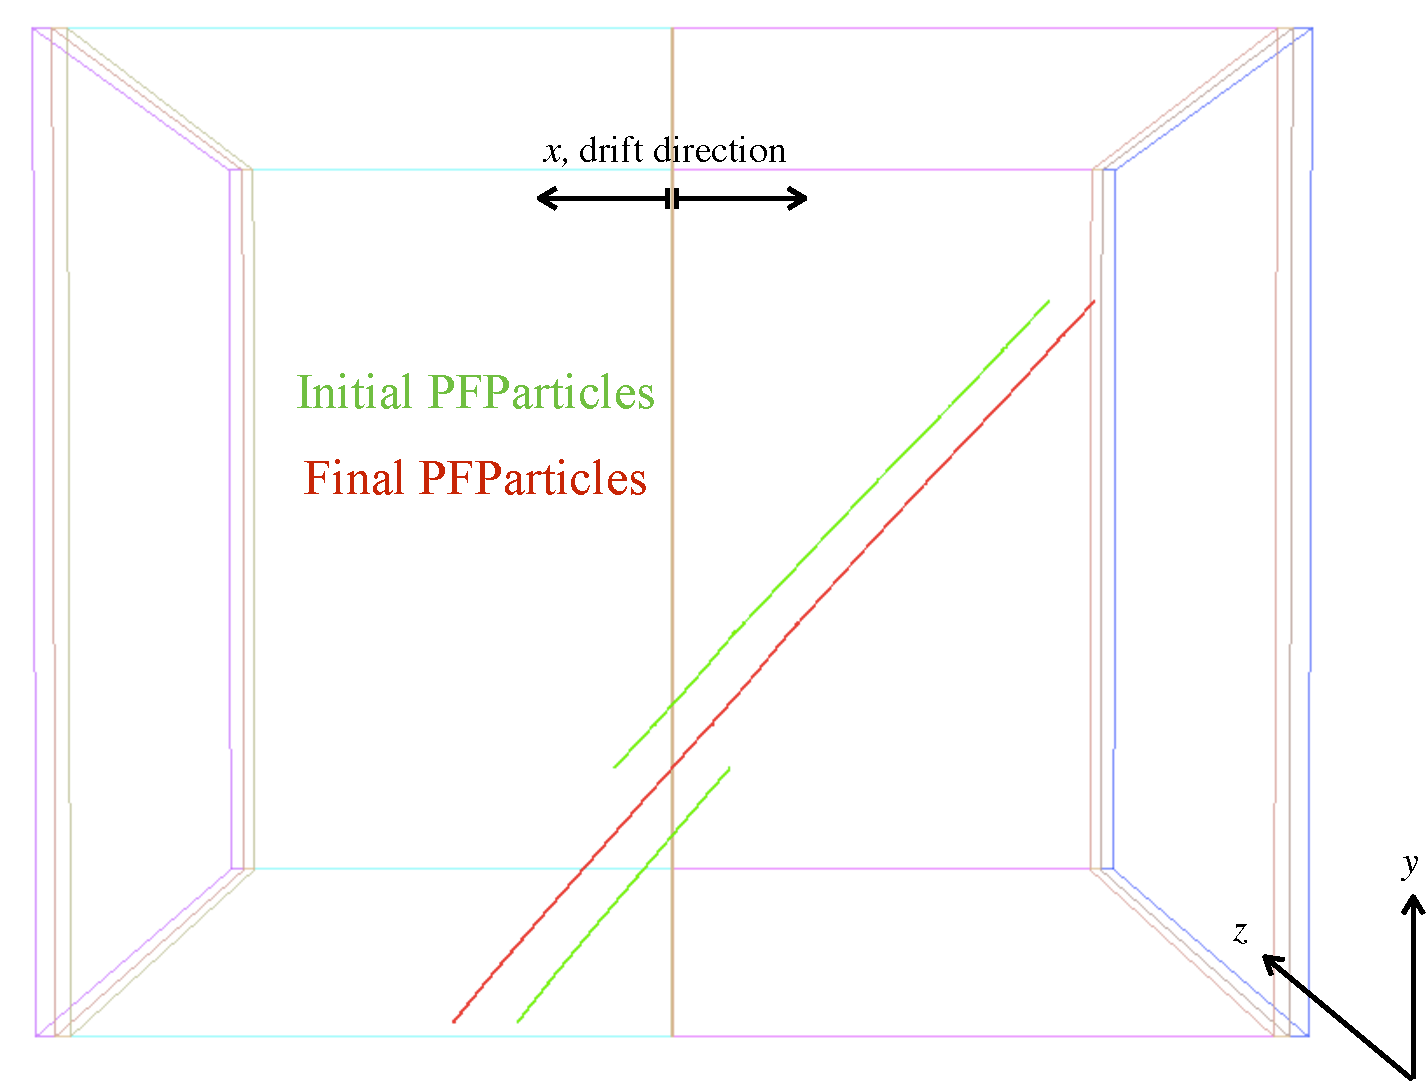
\includegraphics[width=0.75\textwidth]{Figures/EventDisplays/Stitching/StitchingExample.pdf}
\caption{An example of the stitching procedure.  Particles in green are those identified as belonging to the same true cosmic ray particle, while those in red are the outcome after a shift in drift time has been applied.}
\label{fig:stitching}
\end{figure}

\todo{Label CPA and APA in stitching figure example.}

%Mention stitching here. 

%Reference the MicroBooNE paper.

\subsection{Consolidated Reconstruction}
\label{sec:consolidatedreco}

As the appropriate algorithm chain to apply to any individual parent particle interaction varies depending on whether that particle is a cosmic ray muon or a test beam particle, additional logic beyond that contained in the algorithm chains themselves is needed to apply and persist the appropriate reconstruction. This additional logic is applied within the consolidated reconstruction, which is outlined in figure \ref{fig:consolidatedreco}.  
\begin{figure}
\centering
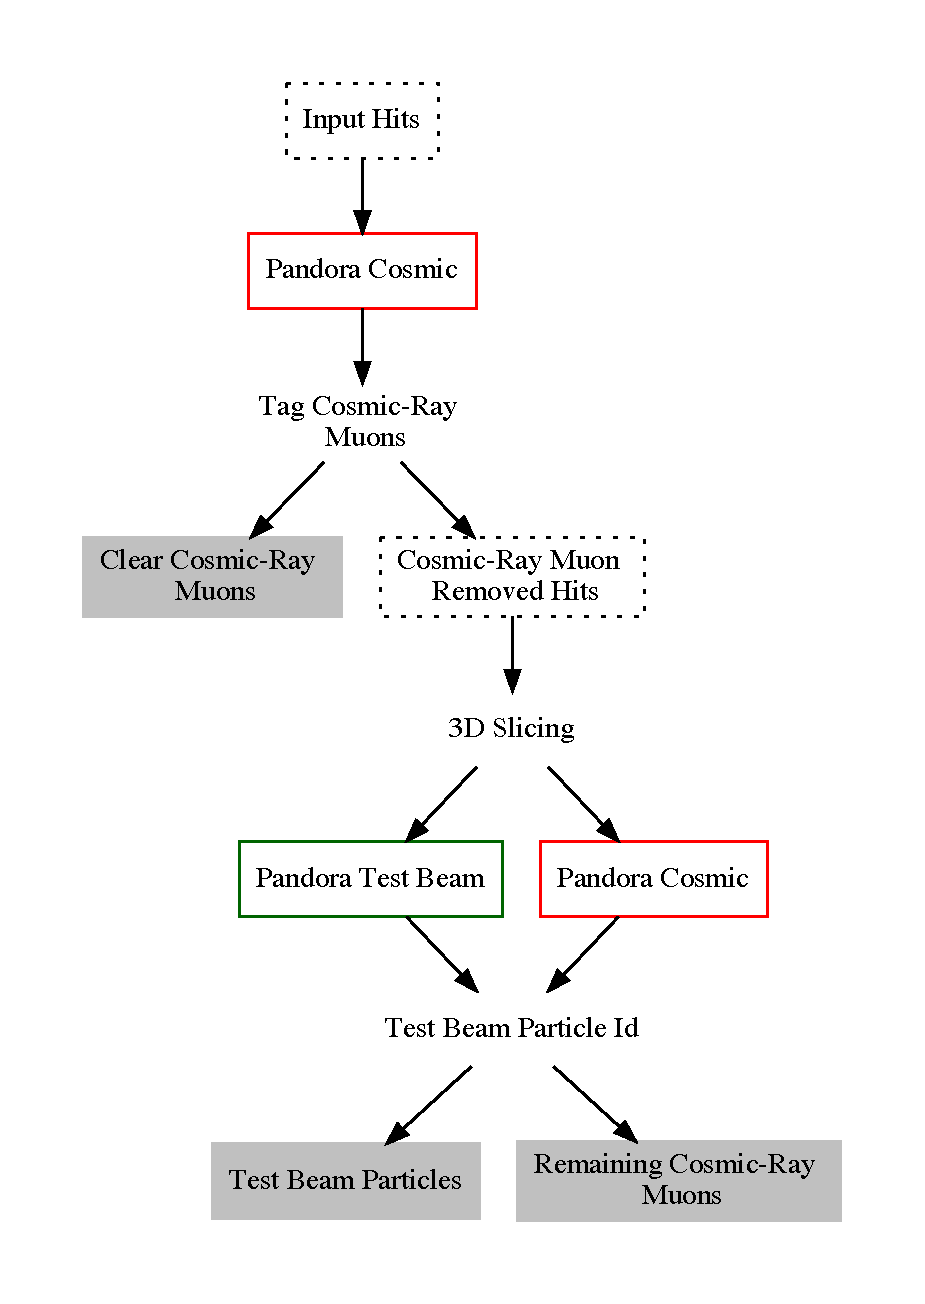
\includegraphics[width=0.5\textwidth]{Figures/Diagram/ConsolidatedReco.pdf}
\caption{Outline of the Pandora consolidated reconstruction.}
\label{fig:consolidatedreco}
\end{figure}

The consolidated reconstruction begins by running the Pandora Cosmic algorithm chain that reconstructs all particles under the cosmic ray particle hypothesis.  The reconstructed particles are then examined in order to determine if they are clear cosmic rays.  Two distinct methods are used for identifying clear cosmic rays:

\begin{itemize}
\item If the hits for the reconstructed particle fall outside the expected read out time window for the target test beam particle.
\item If it the reconstructed particle enters the detector through the top face and exists the lower face.  
\end{itemize}

Reconstructed particles identified as clear cosmic rays are then set aside to form one part of the reconstructed event output and the remaining hits in the event are analyzed further.  These hits are put through a slicing procedure that is designed to group hits together across all three views into regions that contain a single parent particle interaction.  \todo{Picture demonstrating slicing in effect}  Slicing involves running a reduced version of the full reconstruction, where particles are reconstructed up to 3D, but the finesse of particle hierarchies is not considered.  By reconstructing the particles up to 3D, correlations across the three input views are considered when dividing up the event into separate regions, or slices.  This is more powerful than dividing up each view independently.  Each slice is then dissolved back into input hits and the Pandora Test Beam and Cosmic algorithm chains applied independently.  

%\subsubsection{Test Beam Particle ID}
% Not sure whether this needs to be its own subsubsection, but thought it would be sensible to put it in one for now as plots will be needed showing the input distributions and training etc...
At this stage each slice has two possible reconstructed outputs, based on the test beam and cosmic hypotheses respectively.  These reconstruction outputs are then compared in order to determine the most appropriate output to persist.  In ProtoDUNE a BDT is used for this decision.  The following features are used as inputs to the boosted decision tree:

\begin{itemize}
\item The distance of the closest 3D LArTPC hit to the beam spot.
\item The direction and angle of a spatial fit to the reconstructed 3D hits with respect to the beam line.
\item The eigenvalues of the covariance matrix of the spatial position of the 3D LArTPC hits.
\item The vertical distance of the reconstructed 3D LArTPC hit closest to the top of the detector.
\item The number of reconstructed particles.
\end{itemize}

The distribution of the output BDT scores for signal, triggered beam particles, and background, cosmic rays and beam halo, is shown in figure \ref{fig:bdtid} alongside distributions of the selected variables used in the BDT.  The distribution of non-triggered particles does have a peak in the same region as the triggered particles because certain non-triggered beam particles, halo particles from the beam, look topologically similar to signal.  Any slice with a BDT score greater than -0.225 is classified as a test beam particle and the Pandora Test Beam reconstruction output is persisted, while all other slices are reconstructed persisting the Pandora Cosmic hypothesis.  This cut yields a signal efficiency of $99.5 \pm 0.2$\% and a background rejection of $95.3 \pm 0.1$\% in ProtoDUNE-SP simulation.

\begin{figure}
\subfloat[]{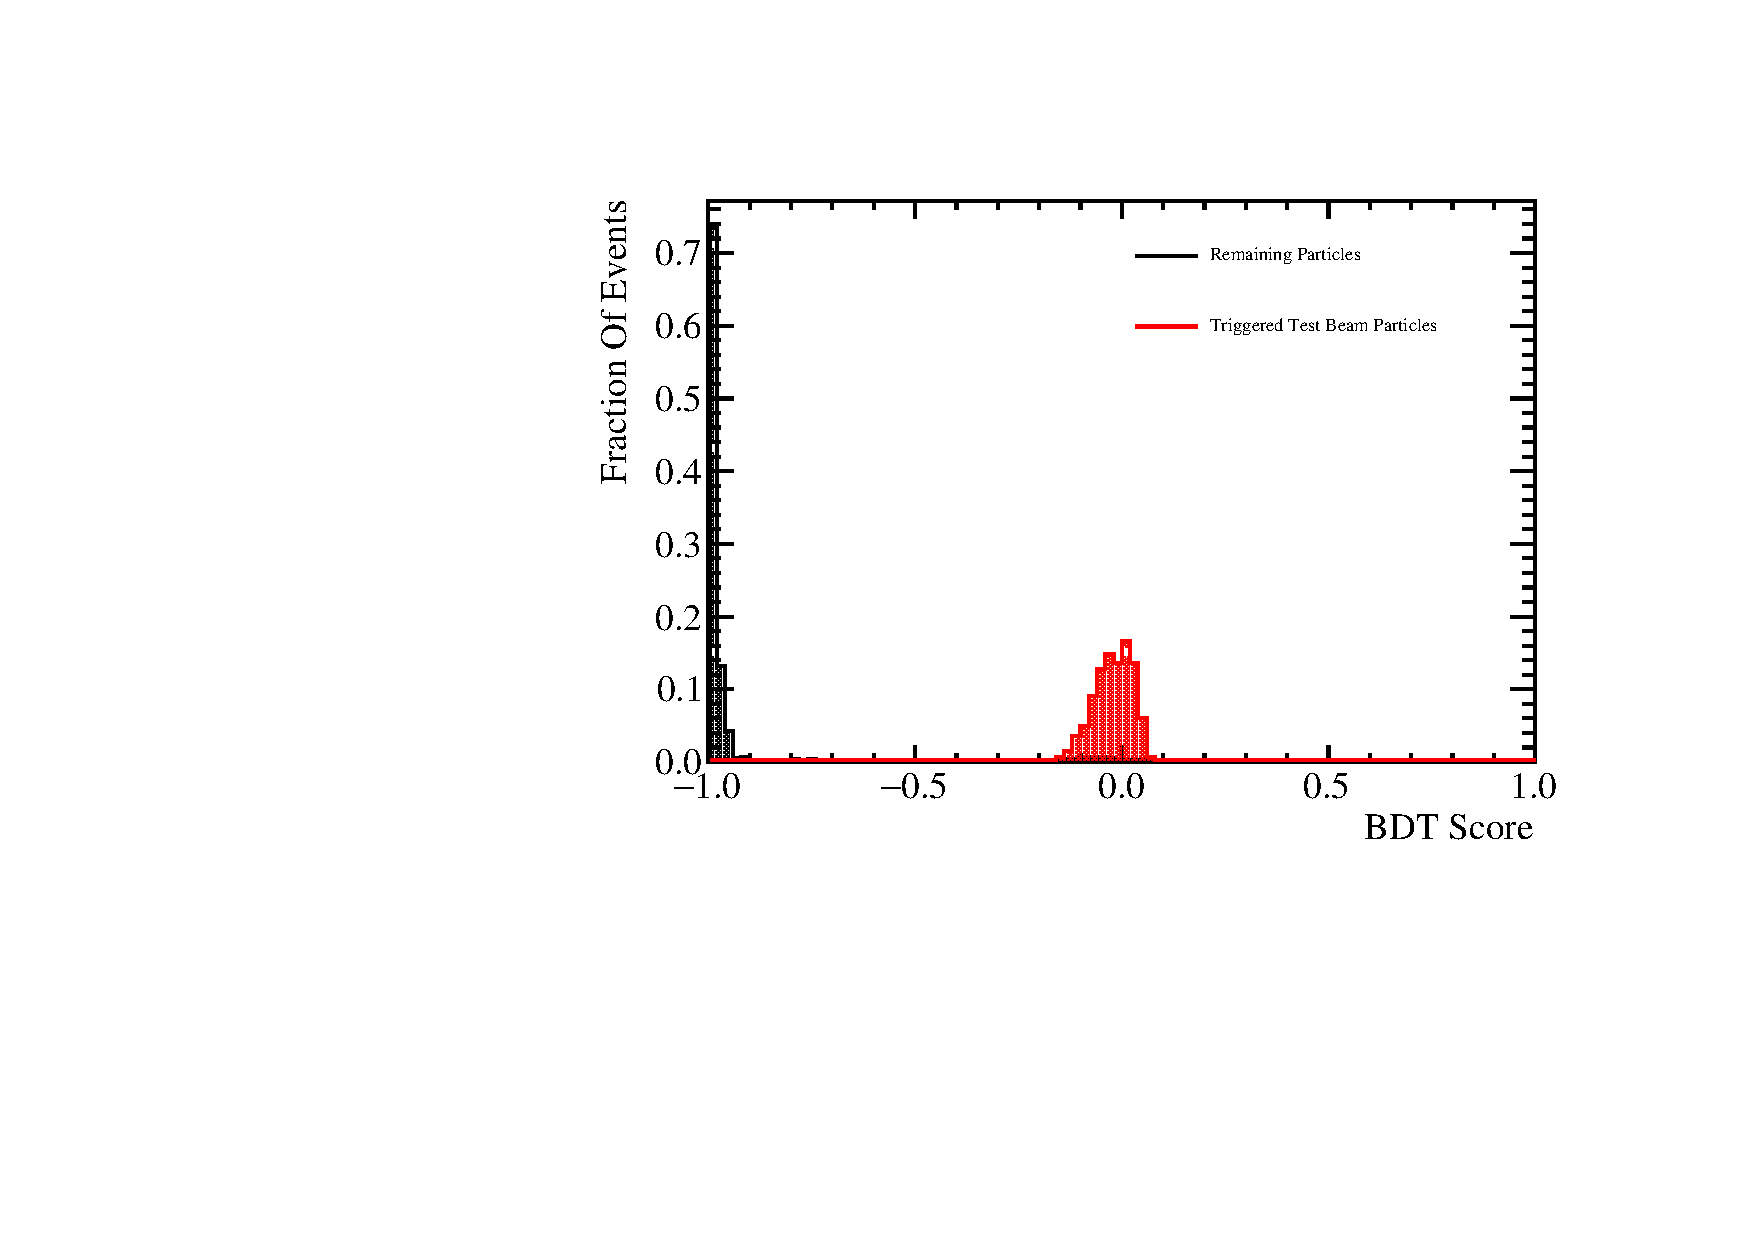
\includegraphics[width=1.0\textwidth]{Figures/TestBeamId/BDTScore.pdf}\label{fig:bdtidscore}} \\
\subfloat[]{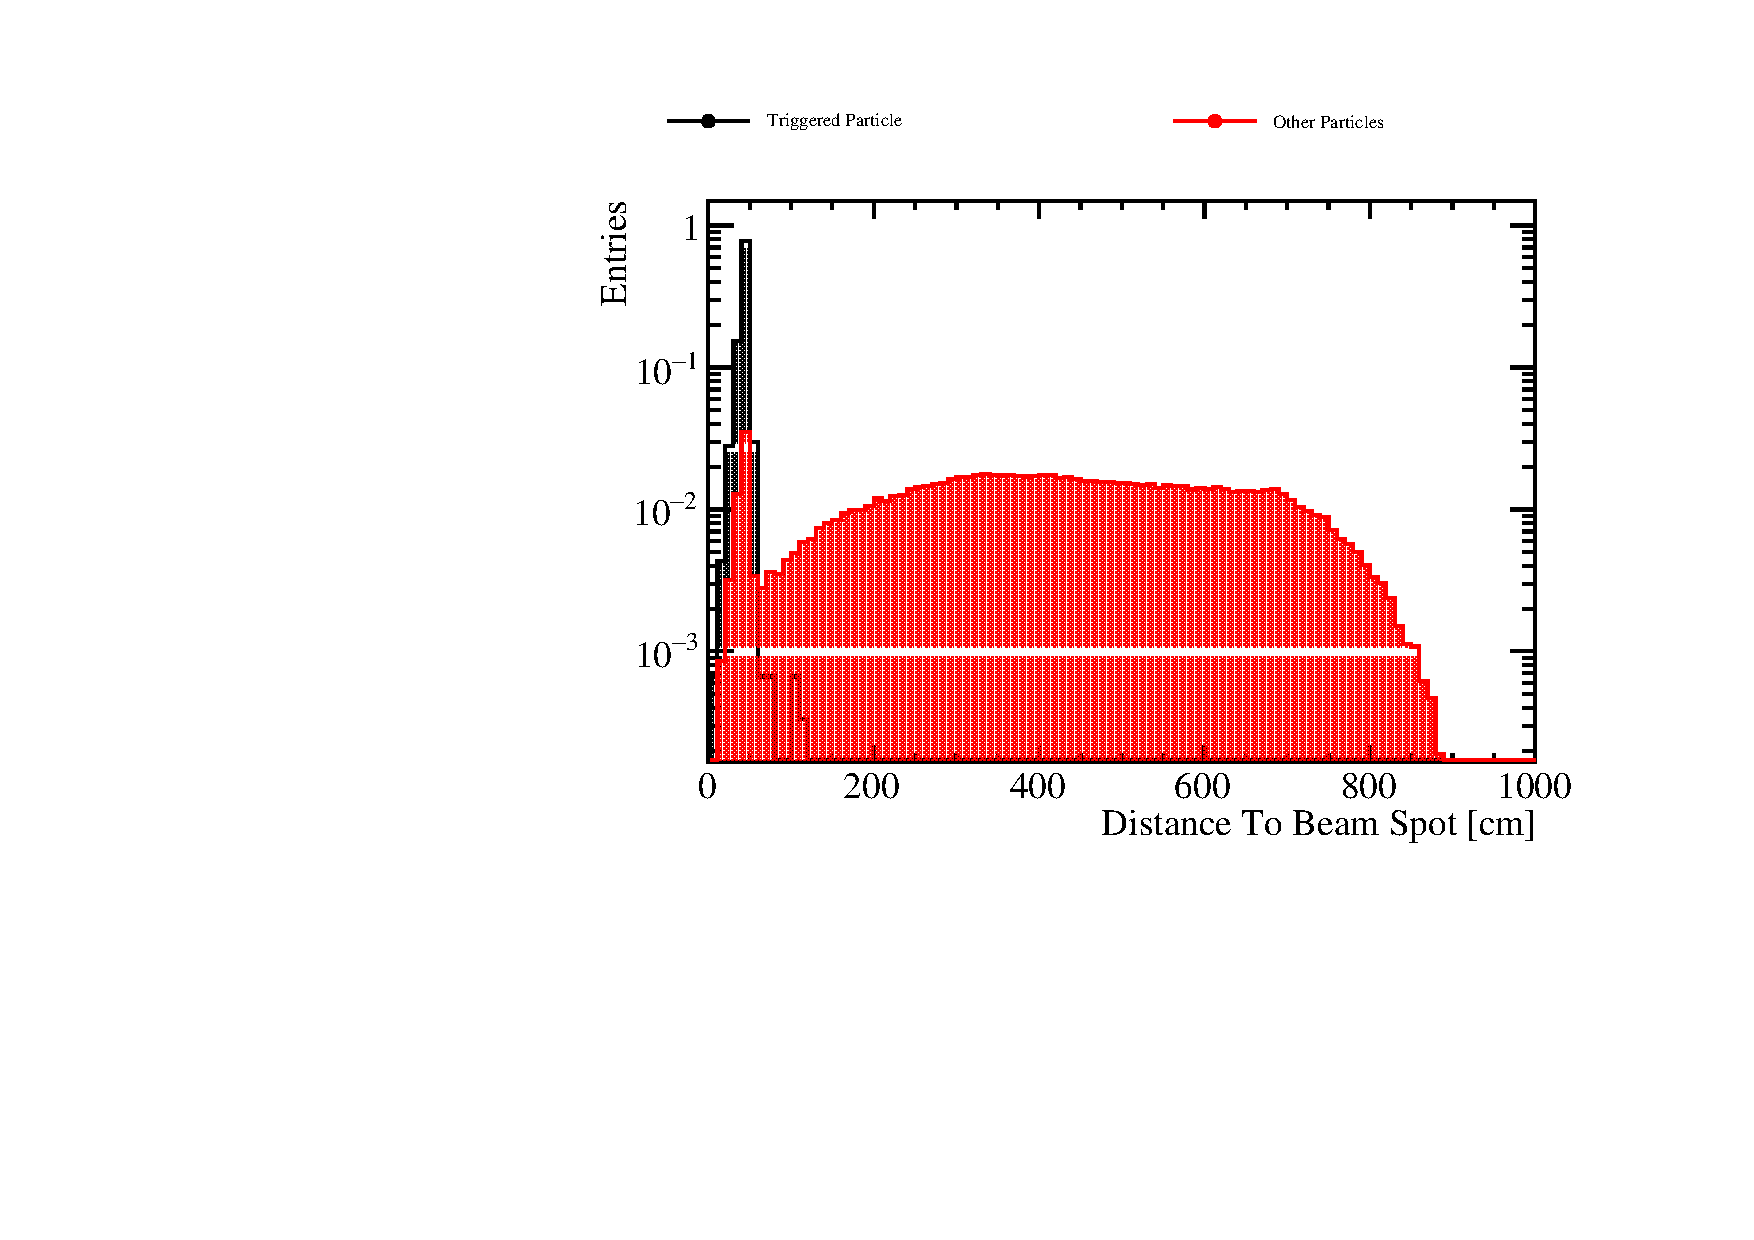
\includegraphics[width=0.33\textwidth]{Figures/TestBeamId/DistanceToBeamSpot.pdf}\label{fig:bdtidvar1}}
\subfloat[]{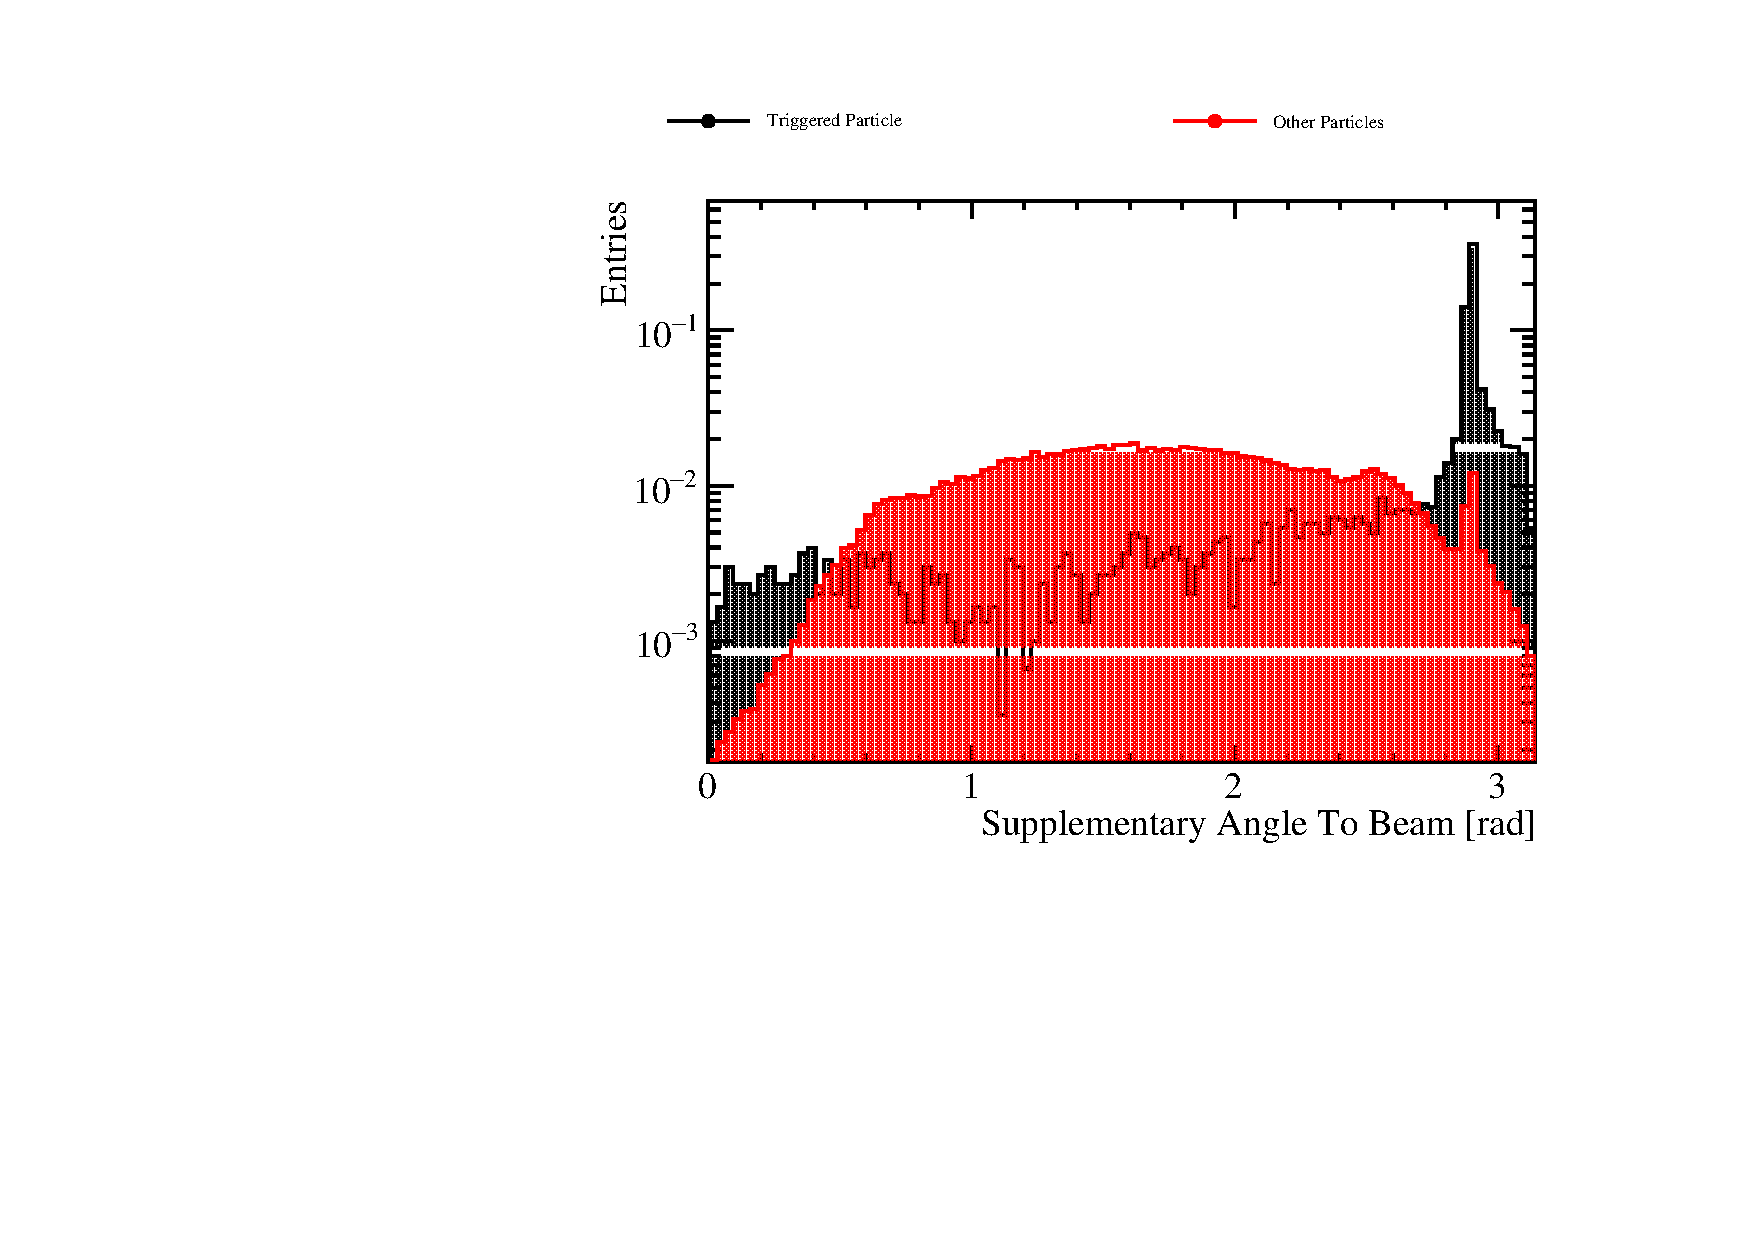
\includegraphics[width=0.33\textwidth]{Figures/TestBeamId/SupplementaryAngleToBeam.pdf}\label{fig:bdtidvar2}}
\subfloat[]{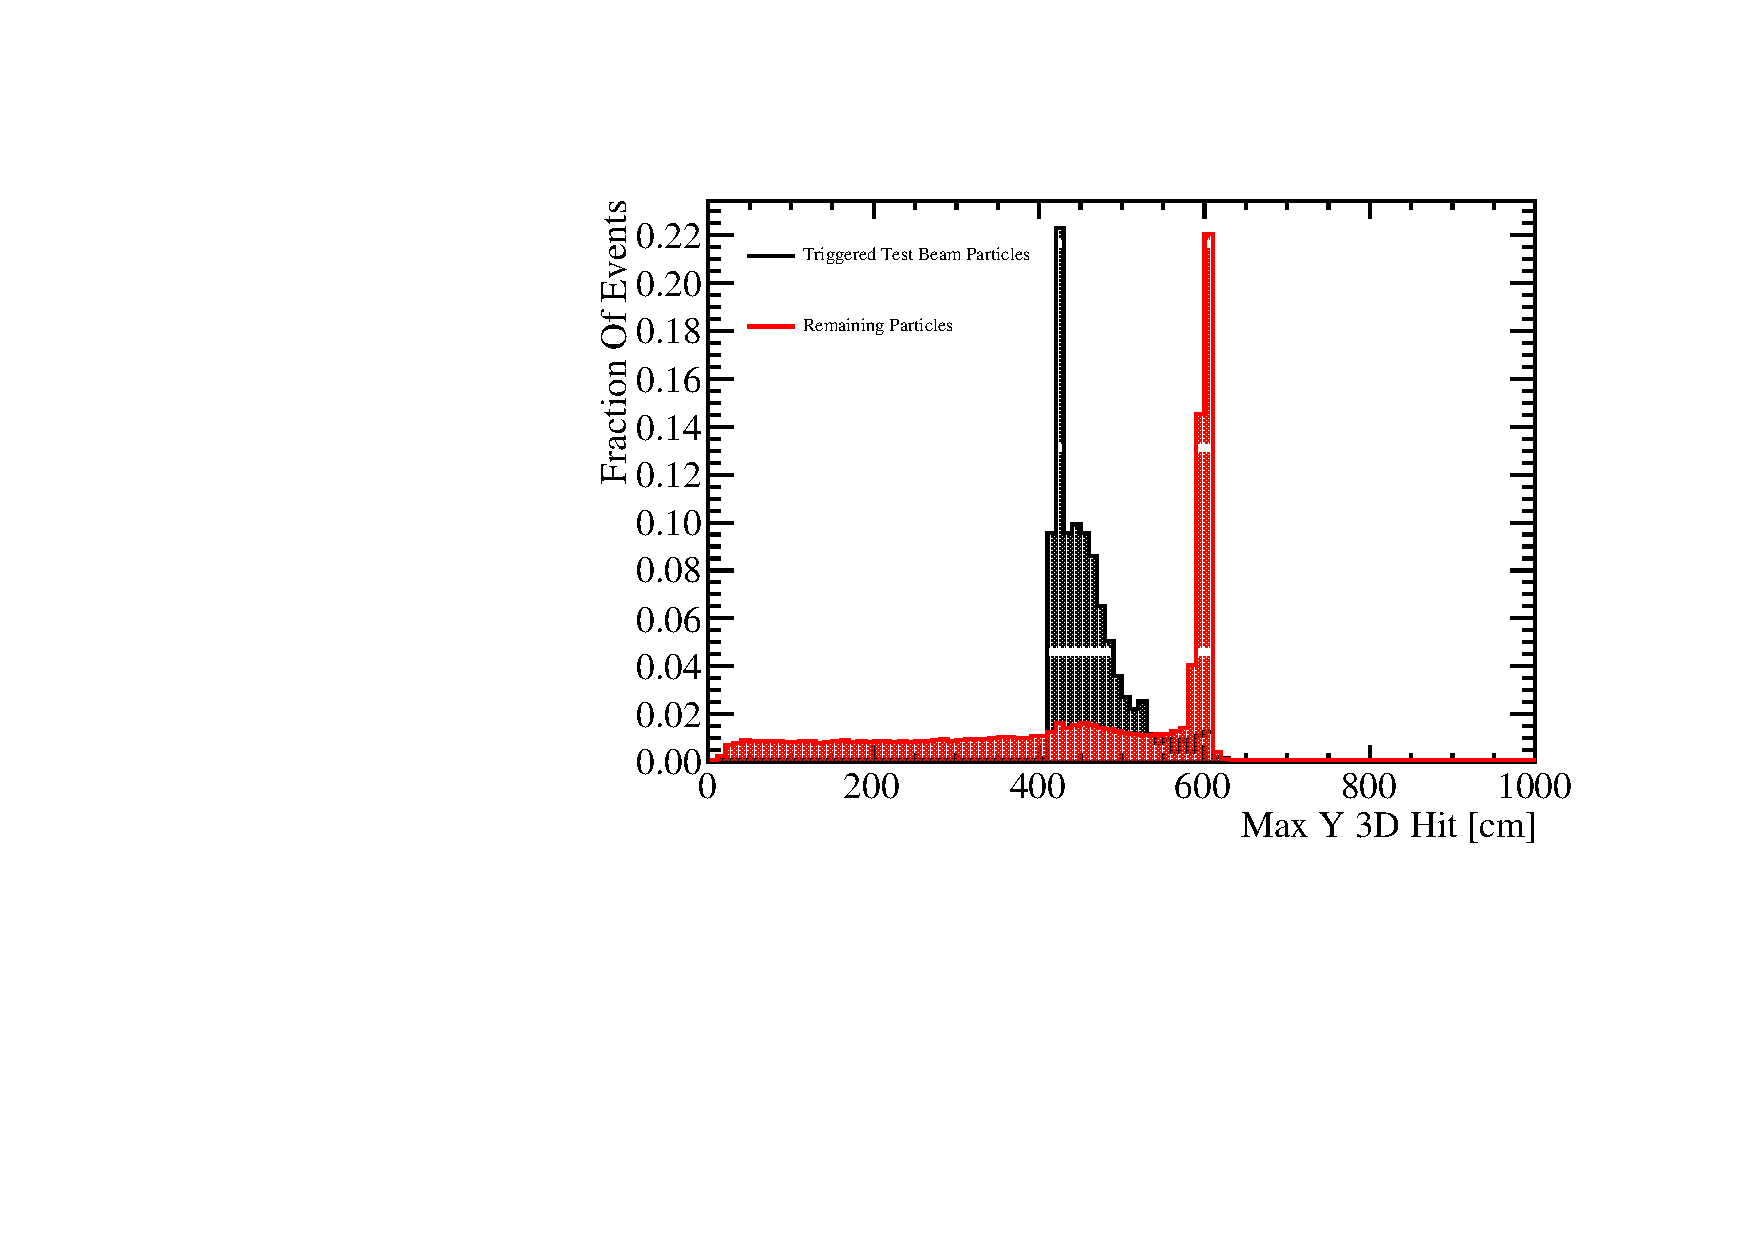
\includegraphics[width=0.33\textwidth]{Figures/TestBeamId/MaxY.pdf}\label{fig:bdtidvar3}}
\caption{The distribution of the BDT score for triggered particles and all remaining particles for both the training and test samples is shown in figure \ref{fig:bdtidscore}.  Figures \ref{fig:bdtidvar1}, \ref{fig:bdtidvar2} and \ref{fig:bdtidvar3} show distributions of selected variables in the BDT used in the test beam id step.  These variables were calculated using the test beam reconstruction for the slice, however, the corresponding variables obtained using the cosmic ray reconstruction are also propagated into the BDT training step.}
\label{fig:bdtid}
\end{figure}

Figure \ref{fig:examplemcreco} shows an example of the reconstruction output for a simulated ProtoDUNE-SP event, where the test beam particle has been correctly identified from the dense cosmic ray background.  Alongside the 3D reconstructed output, this figure also shows the hits identified as being from the test beam particle in the $u$, $v$ and $w$ views.  These 2D vies provides a clear demonstration of how correlating features between the three views can help to resolve possible ambiguities that would be present when considering each view independently.  

\begin{figure}
\centering
\subfloat[]{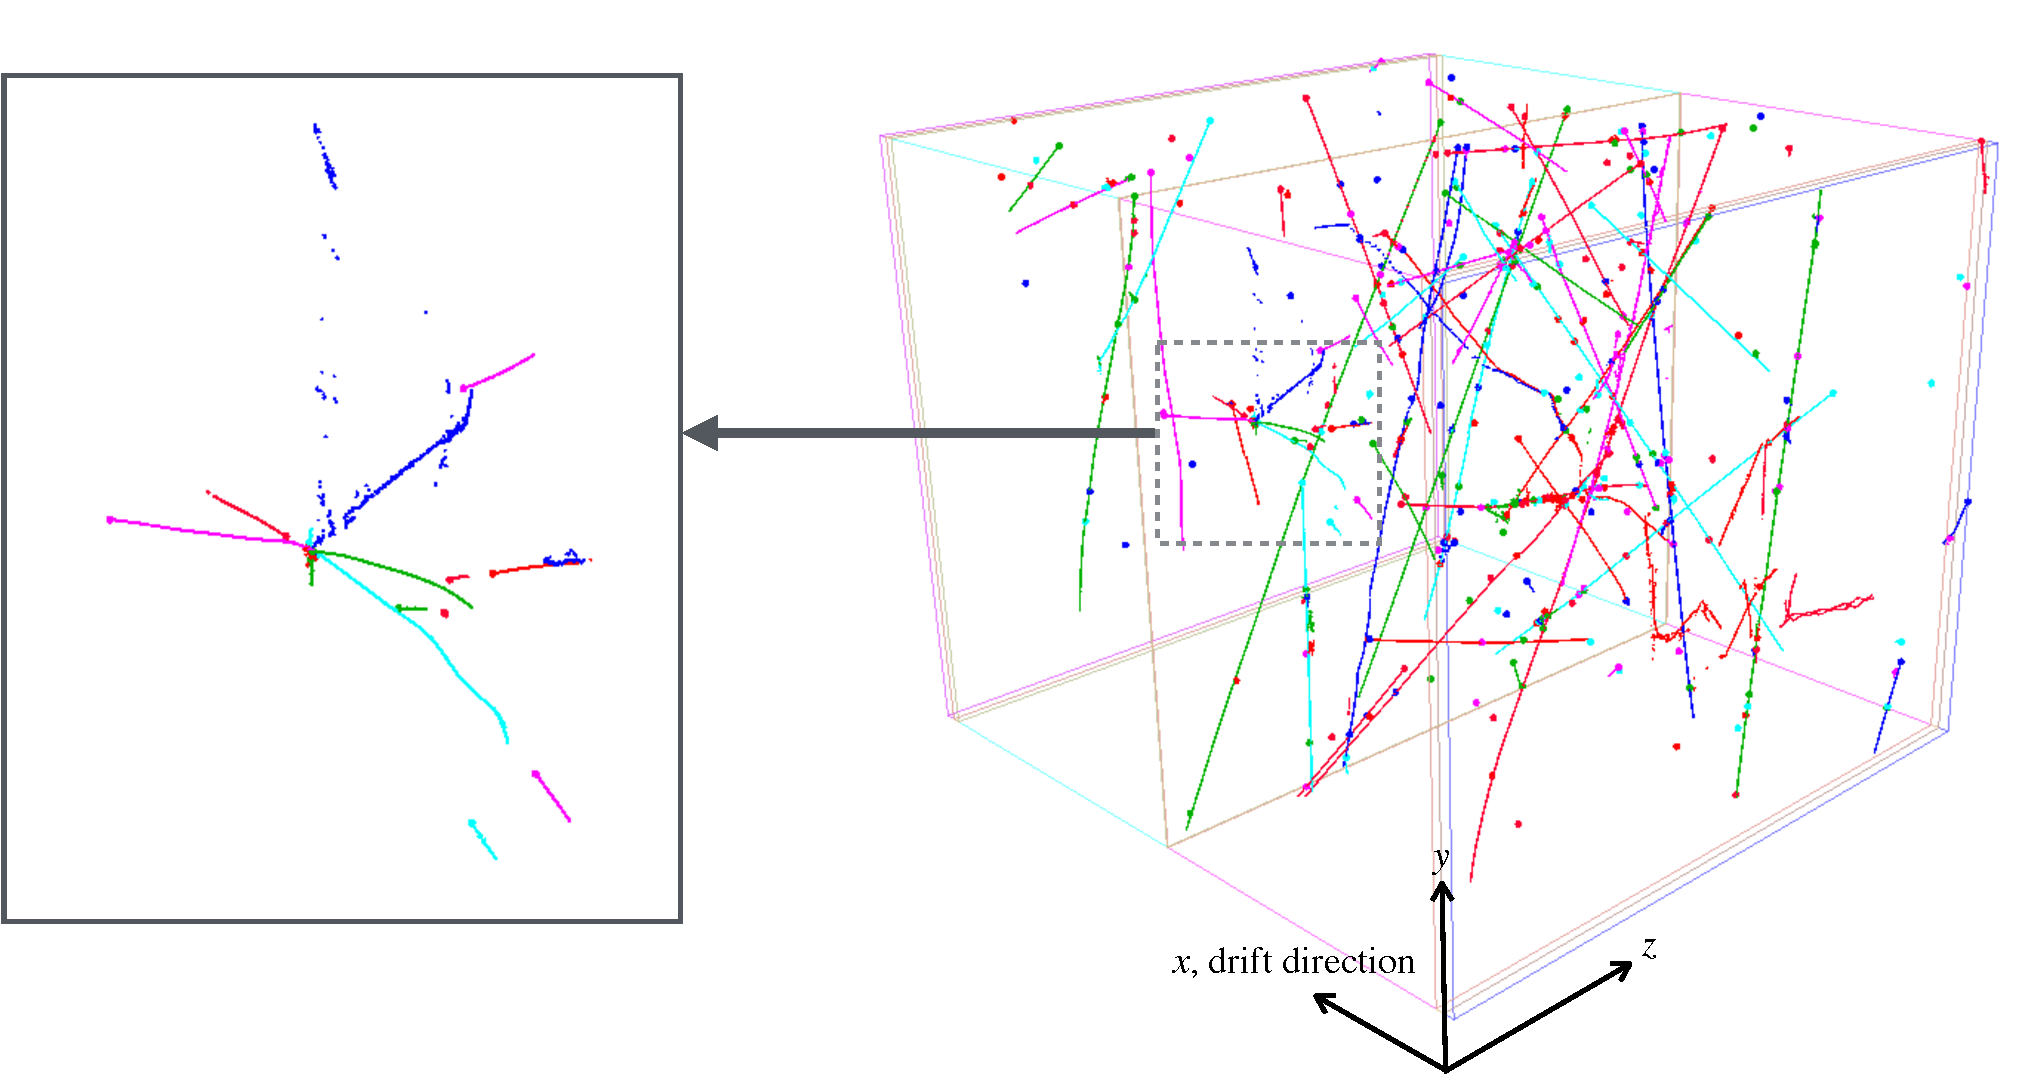
\includegraphics[width=0.75\textwidth]{Figures/EventDisplays/MC/Reconstruction.pdf}\label{fig:examplemcrecoa}} \\
\subfloat[]{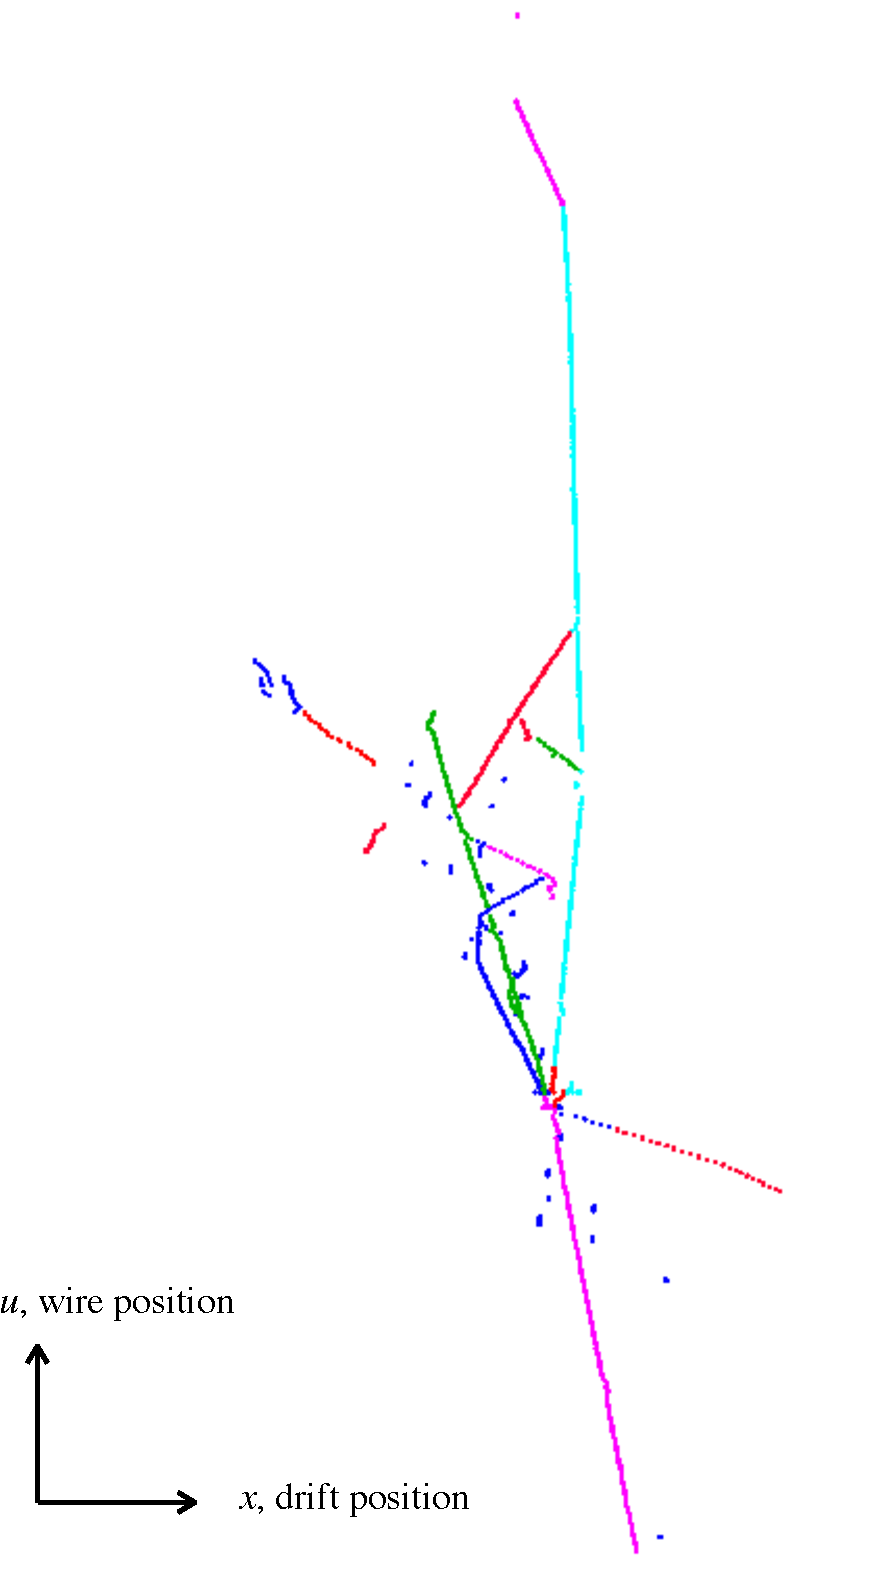
\includegraphics[width=0.3\textwidth]{Figures/EventDisplays/MC/ReconstructionU.pdf}\label{fig:examplemcrecob}}
\subfloat[]{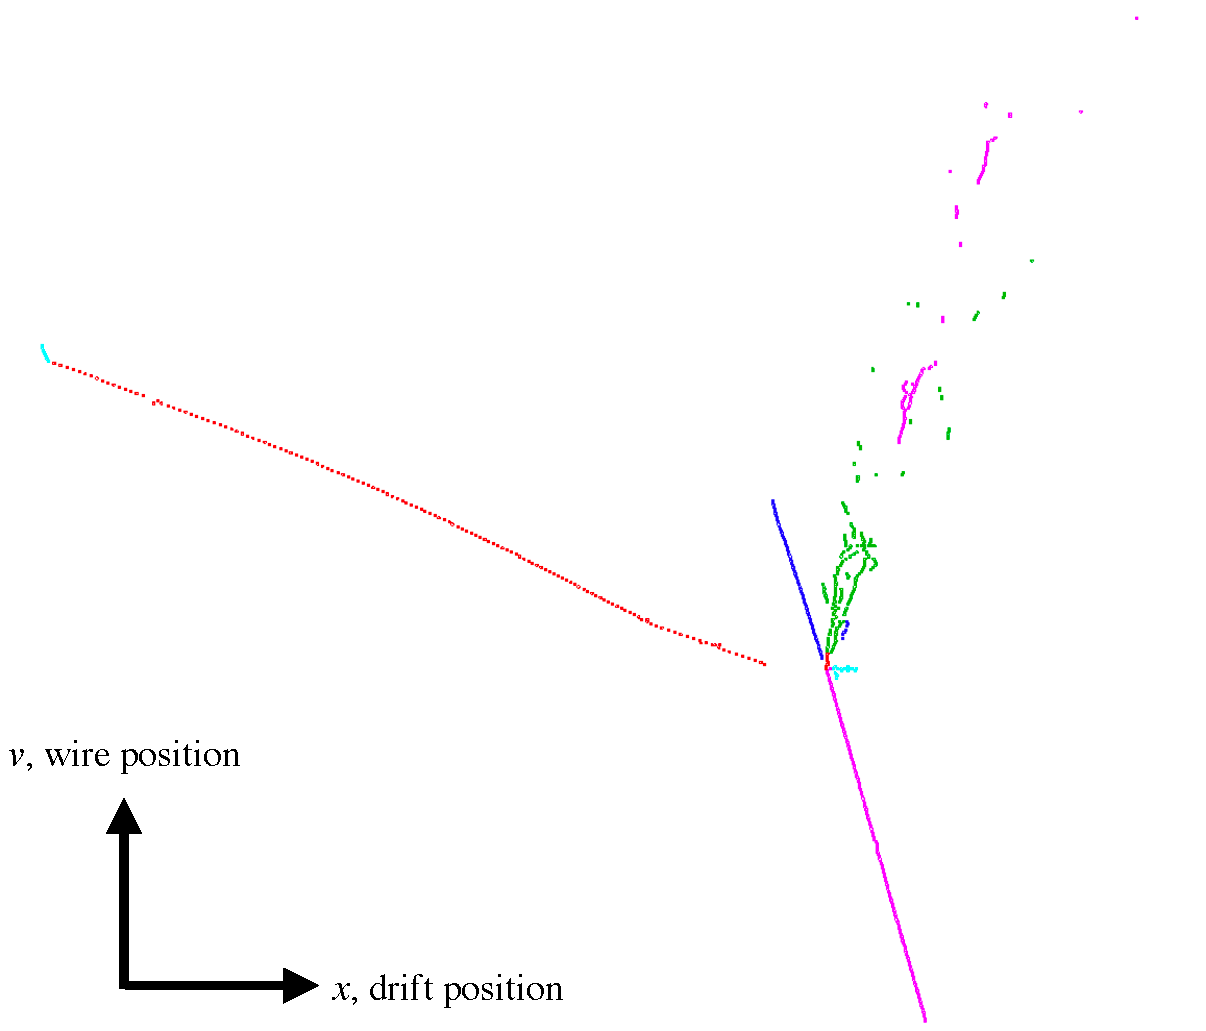
\includegraphics[width=0.3\textwidth]{Figures/EventDisplays/MC/ReconstructionV.pdf}\label{fig:examplemcrecoc}}
\subfloat[]{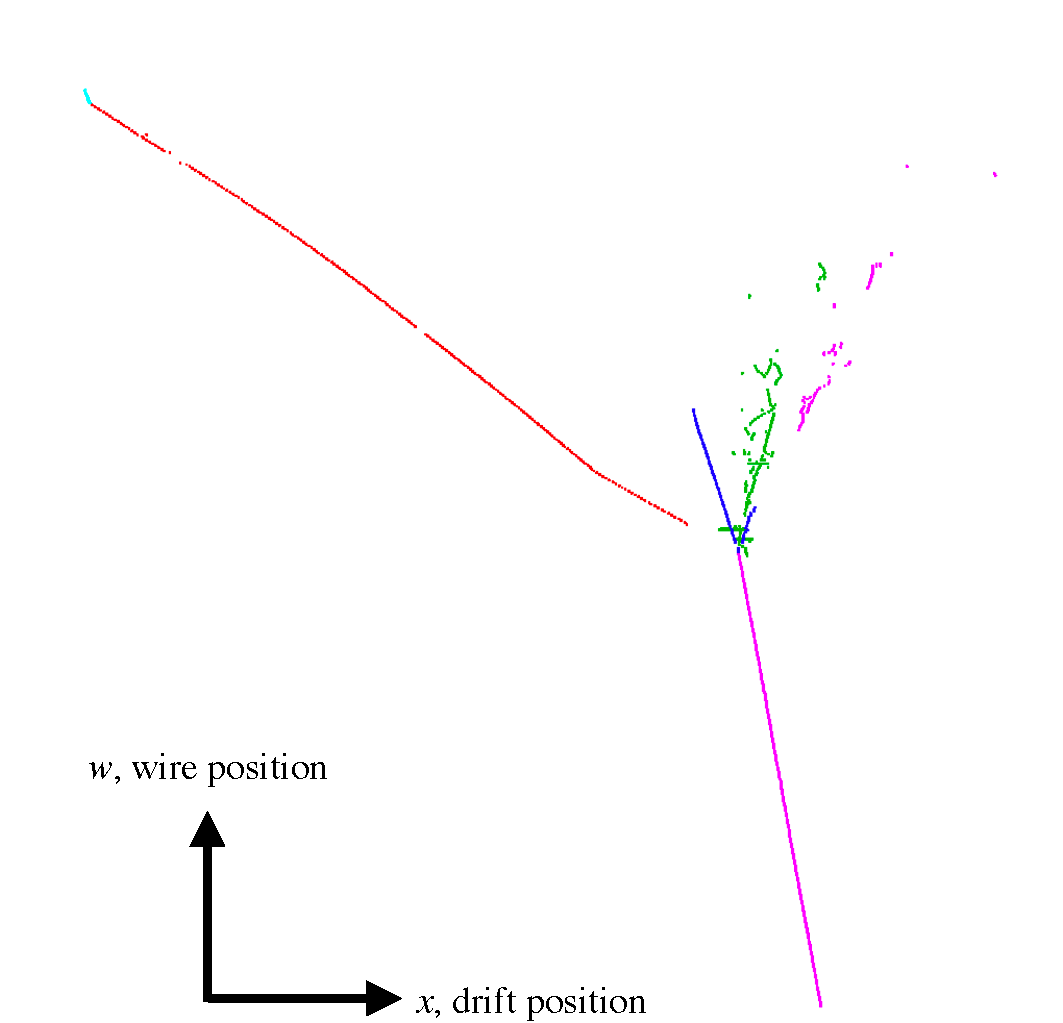
\includegraphics[width=0.3\textwidth]{Figures/EventDisplays/MC/ReconstructionW.pdf}\label{fig:examplemcrecod}} 
\caption{An example of the reconstruction output for a simulated MC 7 GeV $\pi^{+}$ event at ProtoDUNE-SP.  Figure \ref{fig:examplemcrecoa} shows the 3D reconstruction output, highlighting a reconstructed particle identified as a test beam particle interaction, while figures \ref{fig:examplemcrecob}, \ref{fig:examplemcrecoc} and \ref{fig:examplemcrecod} show the $u$, $v$ and $w$ view hits respectively for that reconstructed test beam particle.}
\label{fig:examplemcreco}
\end{figure}

\section{Assessment of Pattern Recognition}
\label{sec:assesmentpatrec}
Validating pattern recognition performance is essential in order for Pandora to provide a high quality reconstruction ready for physics analyses.  

\subsection{Monte-Carlo}
\label{sec:mcmetrics}
For ProtoDUNE-SP a mirrored approach to that taken for evaluating the performance at MicroBooNE was taken \cite{pandorauboone}.  This involves matching MCParticles with reconstructed particles based on the number of shared hits.  

\todo{This is very similar to the MicroBooNE paper, but the metrics are key so I am reluctant to purely cite.  For now go with similar text and figure out plan later.}

Before evaluating performance metrics, a selection of cuts are applied in order to ensure that the MC particles referenced are reconstructable, that is the MC particle must produce a sufficient number of hits in the detector and must not produce an isolated and diffuse topology.  In detail these cuts require that the MC particle produced at least 15 hits in the detector with at least 5 hits in two of the three views.  Furthermore, MC particle hits produced downstream of a far travelling neutron, or, if the target particle is track-like, a far-travelling photon, are removed to veto topologies involving low energy particles being captured and nuclear excitation producing neutrons and photons.

Once these matches have been made the following metrics can be defined:

\begin{itemize}
    \item Efficiency : The fraction of MCParticles that are matched to at least one reconstructed particle.
    \item Purity : For a given pairing, the fraction of hits in the reconstructed particle that are shared with the MCParticle.
    \item Completeness : For a given pairing, the fraction of hits in the MCParticle that are shared with the reconstructed particle.
\end{itemize}

When MCParticles are matched to reconstructed particles, matches are only made if the purity of the match is greater than 50\% in order to ensure that the reconstructed particle is predominantly associated with a single MCParticle.  Furthermore, a completeness of 10\% is required in order to veto low quality matches.  These cuts are not applied when reporting the completeness and purity of matches.  

When evaluating these metrics, matches are made on an event basis by finding the match involving the largest number of shared hits between the MC and reconstructed particle match.  Once this match is made the MC and reconstructed particles are declared unavailable, preventing further matches to either being made.  This process is then repeated to match all remaining particles in the event.  At this stage all MC and reconstructed particles have at most one match.  Any remaining reconstructed particles that have no match are associated to the MC particle, that by definition must already have a single match, that they share the most hits with irrespective of the number of matches the MCParticle currently has.

\begin{figure}
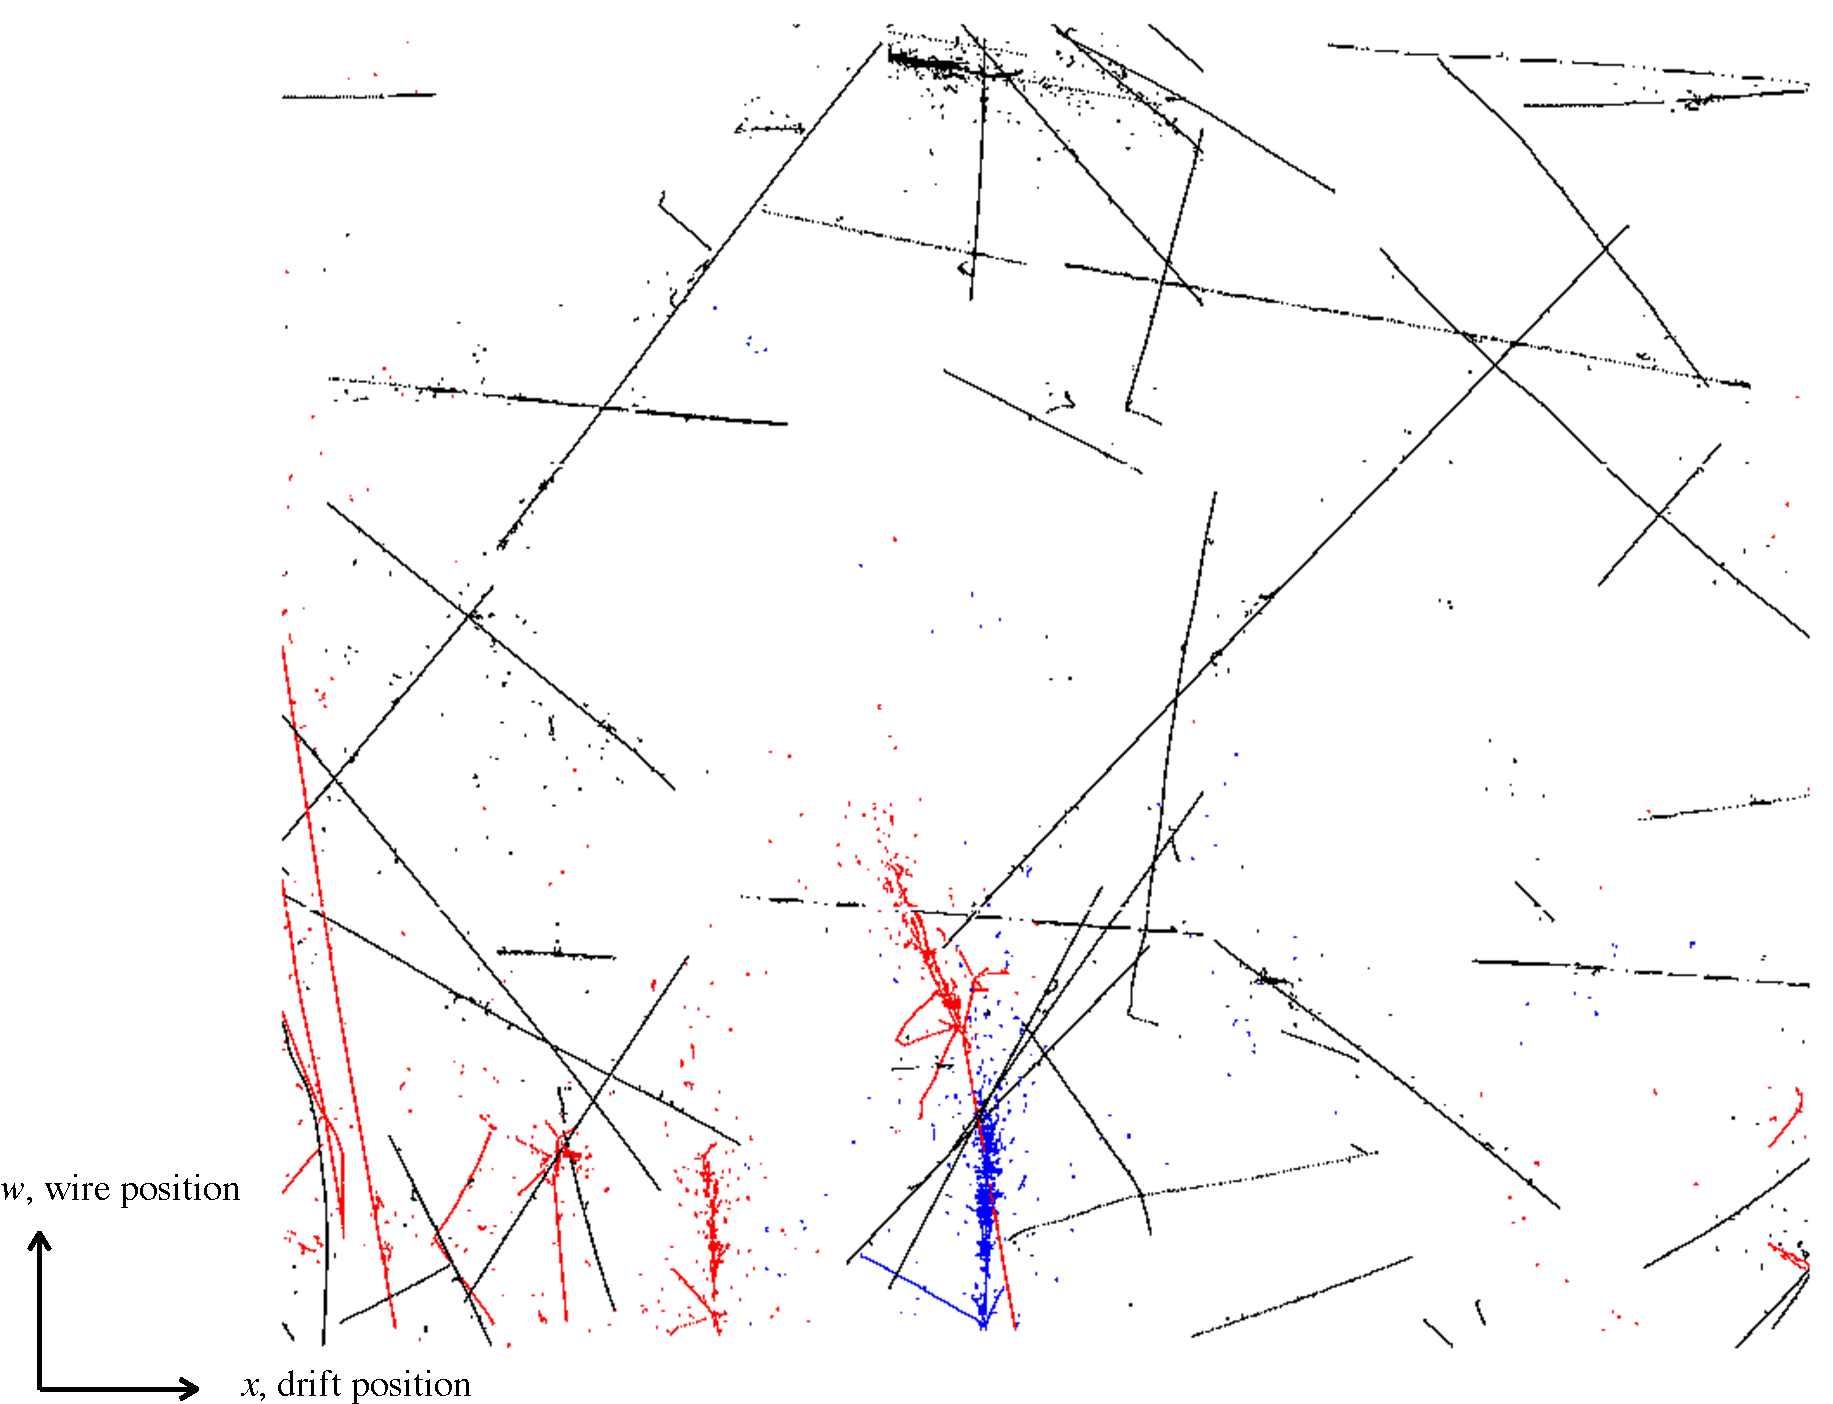
\includegraphics[width=0.75\textwidth]{Figures/EventDisplays/MC/EventComposition.pdf} 
\caption{An example of the reconstruction output for a MC 7 GeV pion event at ProtoDUNE-SP.}
\label{fig:1b}
\end{figure}

\subsubsection{Test Beam Metrics}

Using the MCC11 ProtoDUNE-SP simulation the triggered test beam particle reconstruction was studied. For this sample the breakdown of different particle species is shown in table \ref{tab:mcc11species}.  In order to perform a fair comparison to ProtoDUNE-SP data in following sections, only positively charged triggered test beam particle species are considered.

\begin{table}
\centering
\caption{The number of triggered test beam particle events for the ProtoDUNE-SP MCC11 sample.}
\label{tab:mcc11species} 
\begin{tabular}{cc}
\hline\noalign{\smallskip}
Particle Species & Entries  \\
\noalign{\smallskip}\hline\noalign{\smallskip}
$\pi^{+}$ & 8874 \\
$e^{+}$ & 6699 \\
$p$ & 2164 \\
$K^{+}$ & 452 \\
$\mu^{+}$ & 233 \\
\noalign{\smallskip}\hline
\end{tabular}
\end{table}

Figure \ref{fig:tbrecoeff} shows the reconstruction efficiency for the triggered test beam particles as a function of the number of 2D hits in the detector and the true momentum of the particle.  As the number of hits in the detector increases the reconstruction efficiency increases and eventually plateaus around 1000 hits at 80\%.  The inefficiencies in the reconstruction efficiency originate from cosmic ray and beam halo contamination.  As shown in figure \ref{fig:tbrecoeffbrkdwn}, removing cosmic rays and beam particle halo improves the reconstruction efficiency to an integrated value of 94\%.  The remaining failure mode is inefficiencies in the test beam particle identification step.

Figure \ref{fig:tbrecopurcom} shows the purity and completeness of the reconstructed test beam particle.  Both of these distributions peak at 1, indicating a good reconstruction performance. By referring to figure \ref{fig:tbrecoeffbrkdwn}, it becomes clear that the primary degradation mechanism for purity is mixing of the triggered test beam particle with beam halo overlay, while completeness degrades due to splitting up of the reconstructed test beam particle, even in the absence of any contamination.  \todo{I feel this part needs more, but I don't really know what to say...}

\begin{figure}
\centering
\subfloat[]{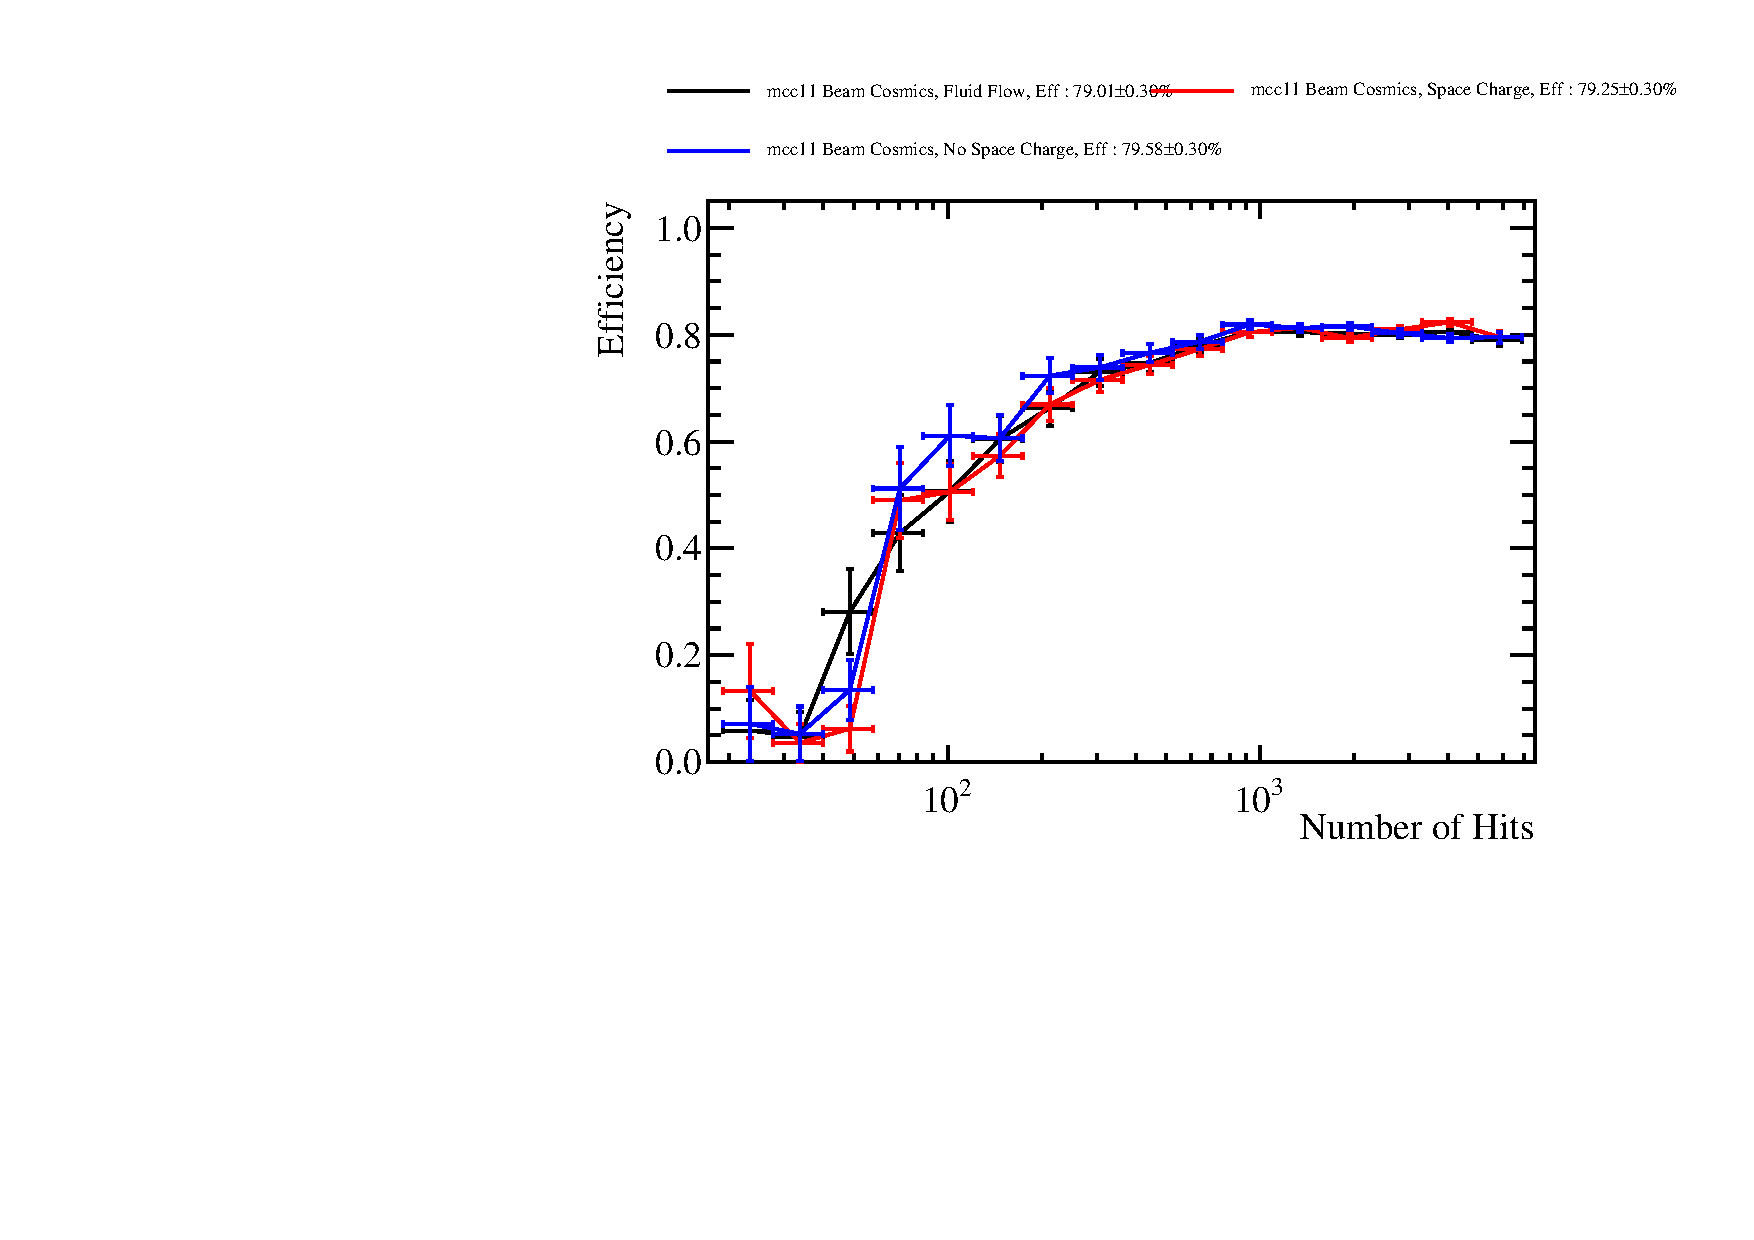
\includegraphics[width=0.45\textwidth]{Figures/Metrics/MC/Beam/BeamParticleEfficiencyBreakdownVsNHits.pdf}\label{fig:tbrecoeffnhits}}
\subfloat[]{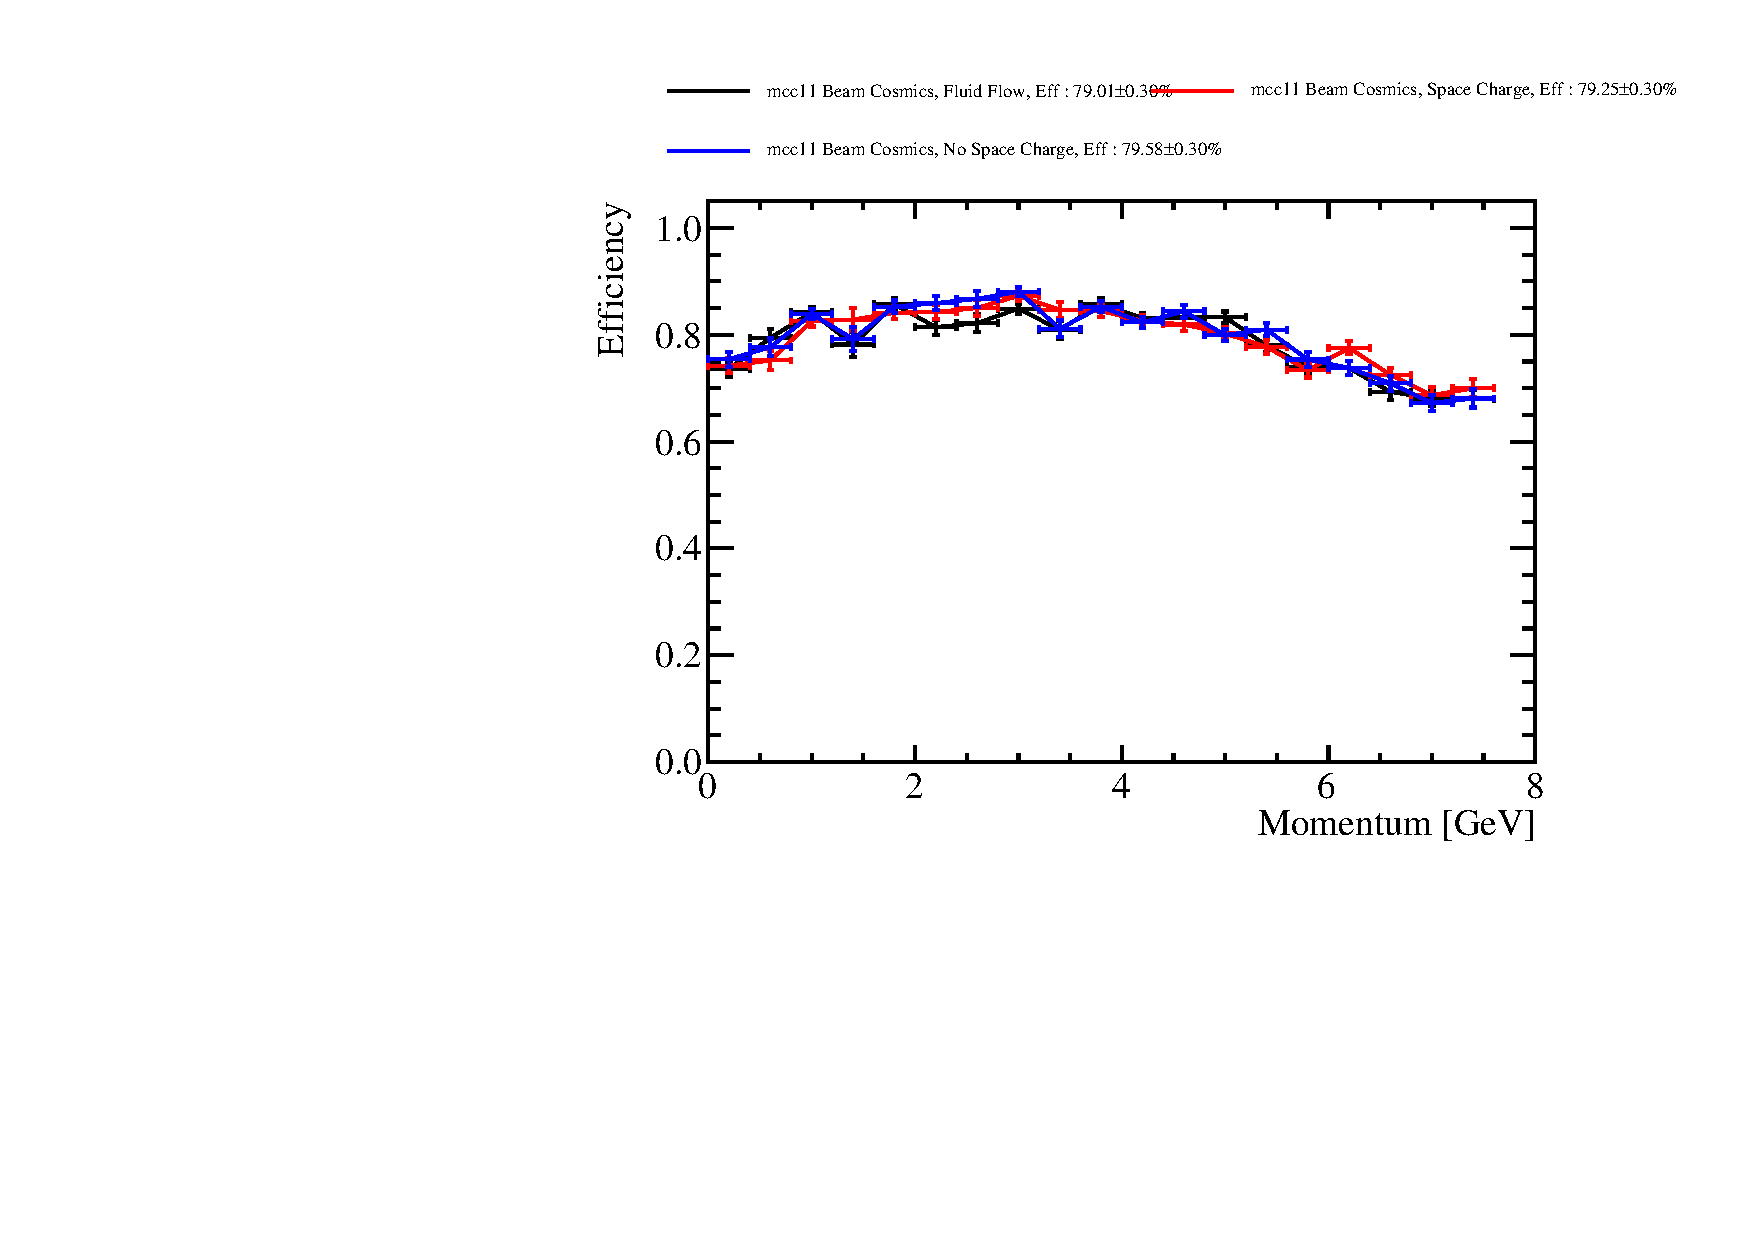
\includegraphics[width=0.45\textwidth]{Figures/Metrics/MC/Beam/BeamParticleEfficiencyBreakdownVsMomentum.pdf}\label{fig:tbrecoeffp}}
\caption{The test beam particle reconstruction efficiency as a function of \subref{fig:tbrecoeffnhits} the number of hits in the test beam particle and \subref{fig:tbrecoeffp} the test beam particle momentum in MC.}
\label{fig:tbrecoeff}
\end{figure}

\begin{figure}
\centering
\subfloat[]{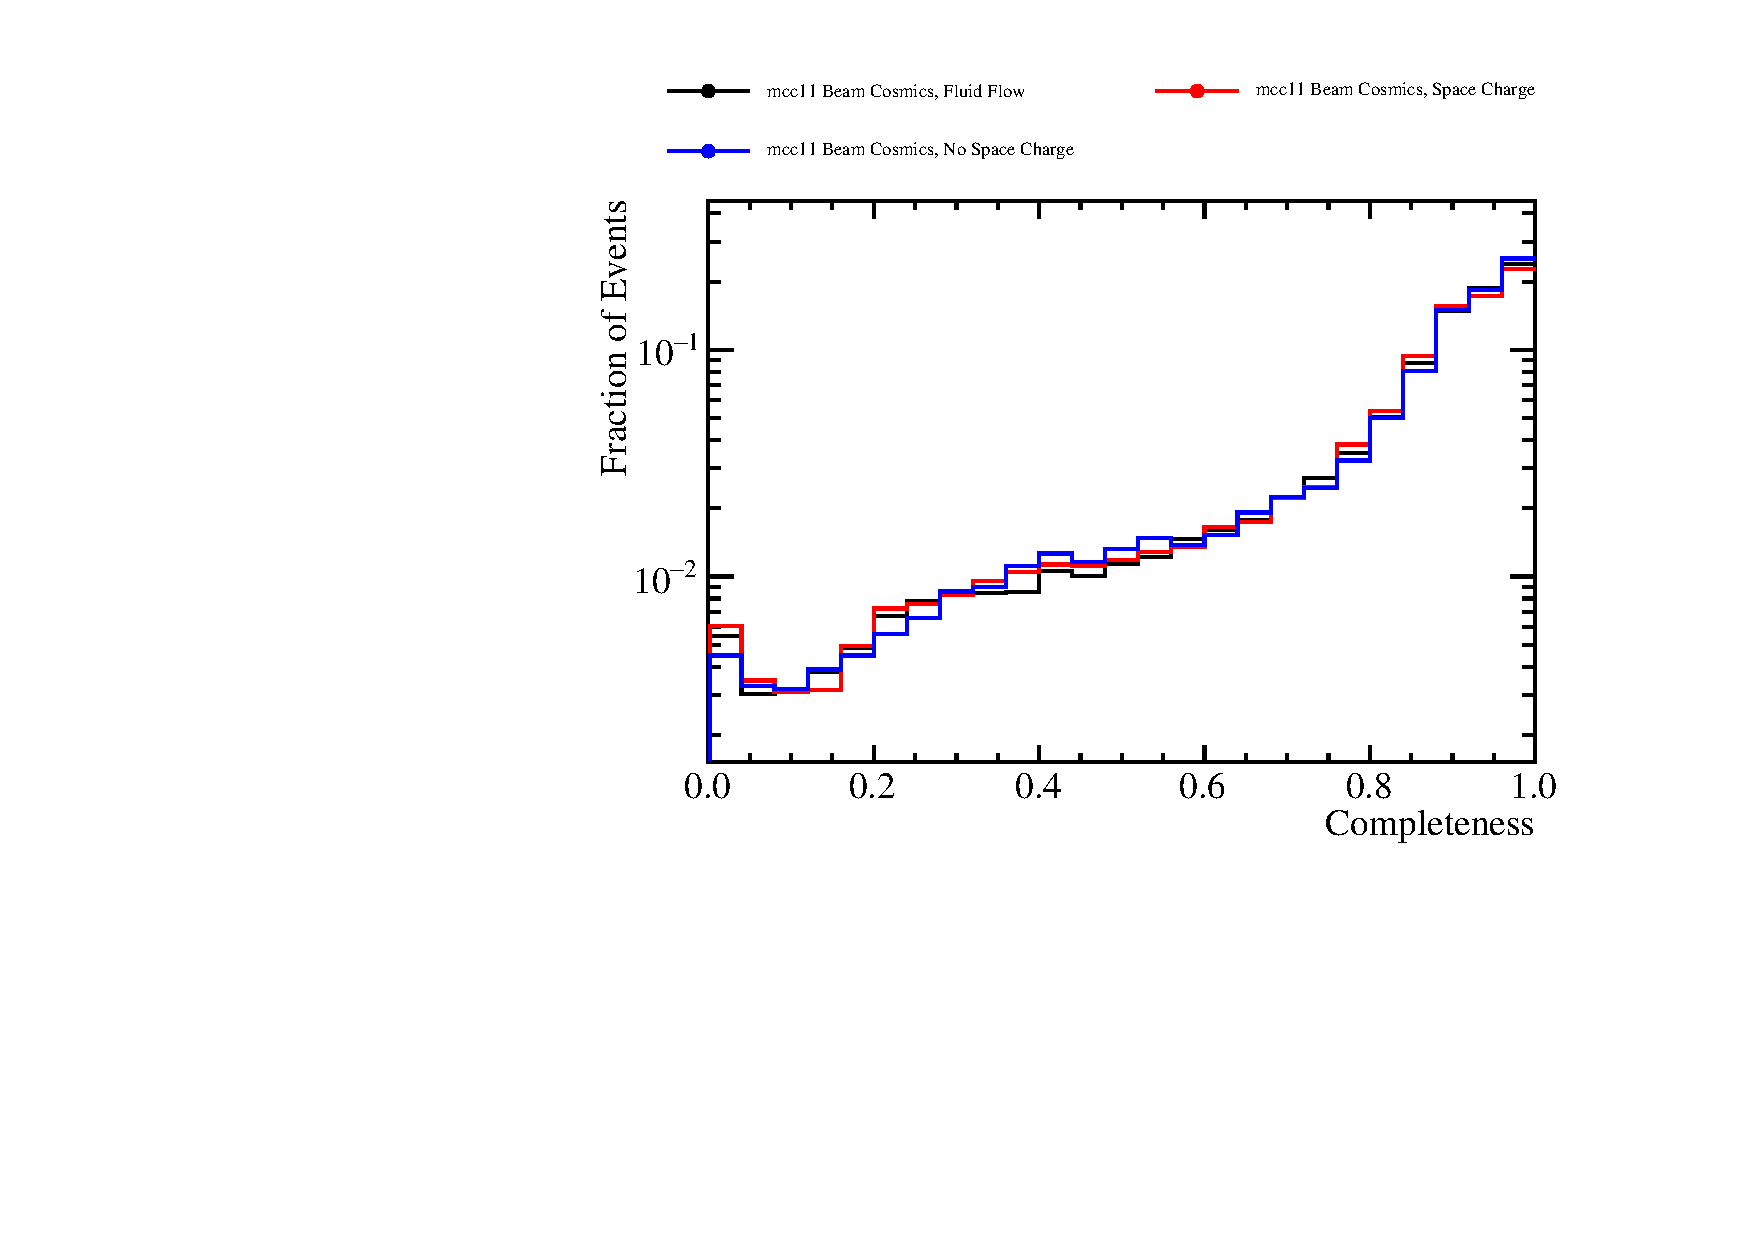
\includegraphics[width=0.45\textwidth]{Figures/Metrics/MC/Beam/BeamParticleCompleteness.pdf}\label{fig:tbrecocomp}}
\subfloat[]{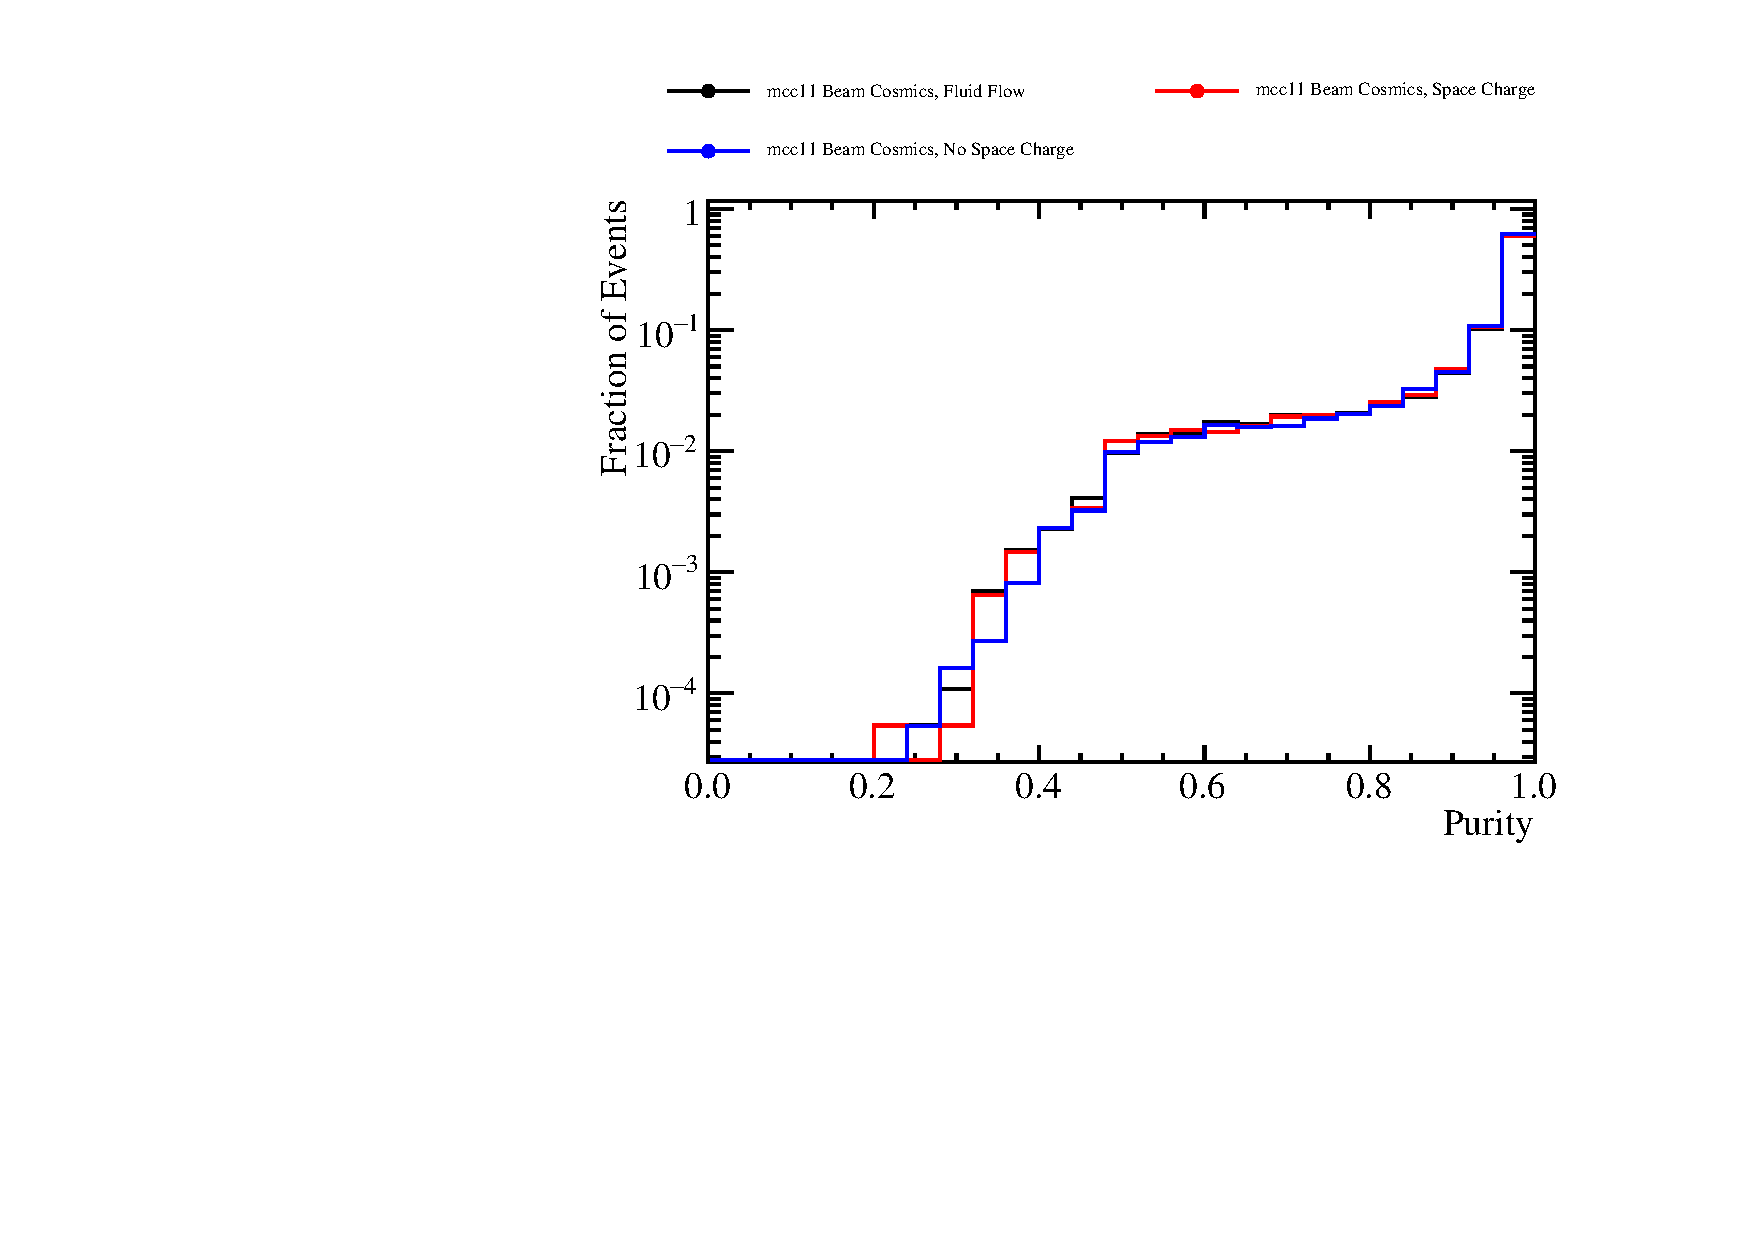
\includegraphics[width=0.45\textwidth]{Figures/Metrics/MC/Beam/BeamParticlePurity.pdf}\label{fig:tbrecopur}}
\caption{\subref{fig:tbrecocomp} The purity and \subref{fig:tbrecopur} completeness of reconstructed test beam particles in simulation.}
\label{fig:tbrecopuritycomp}
\end{figure}

\begin{figure}
\centering
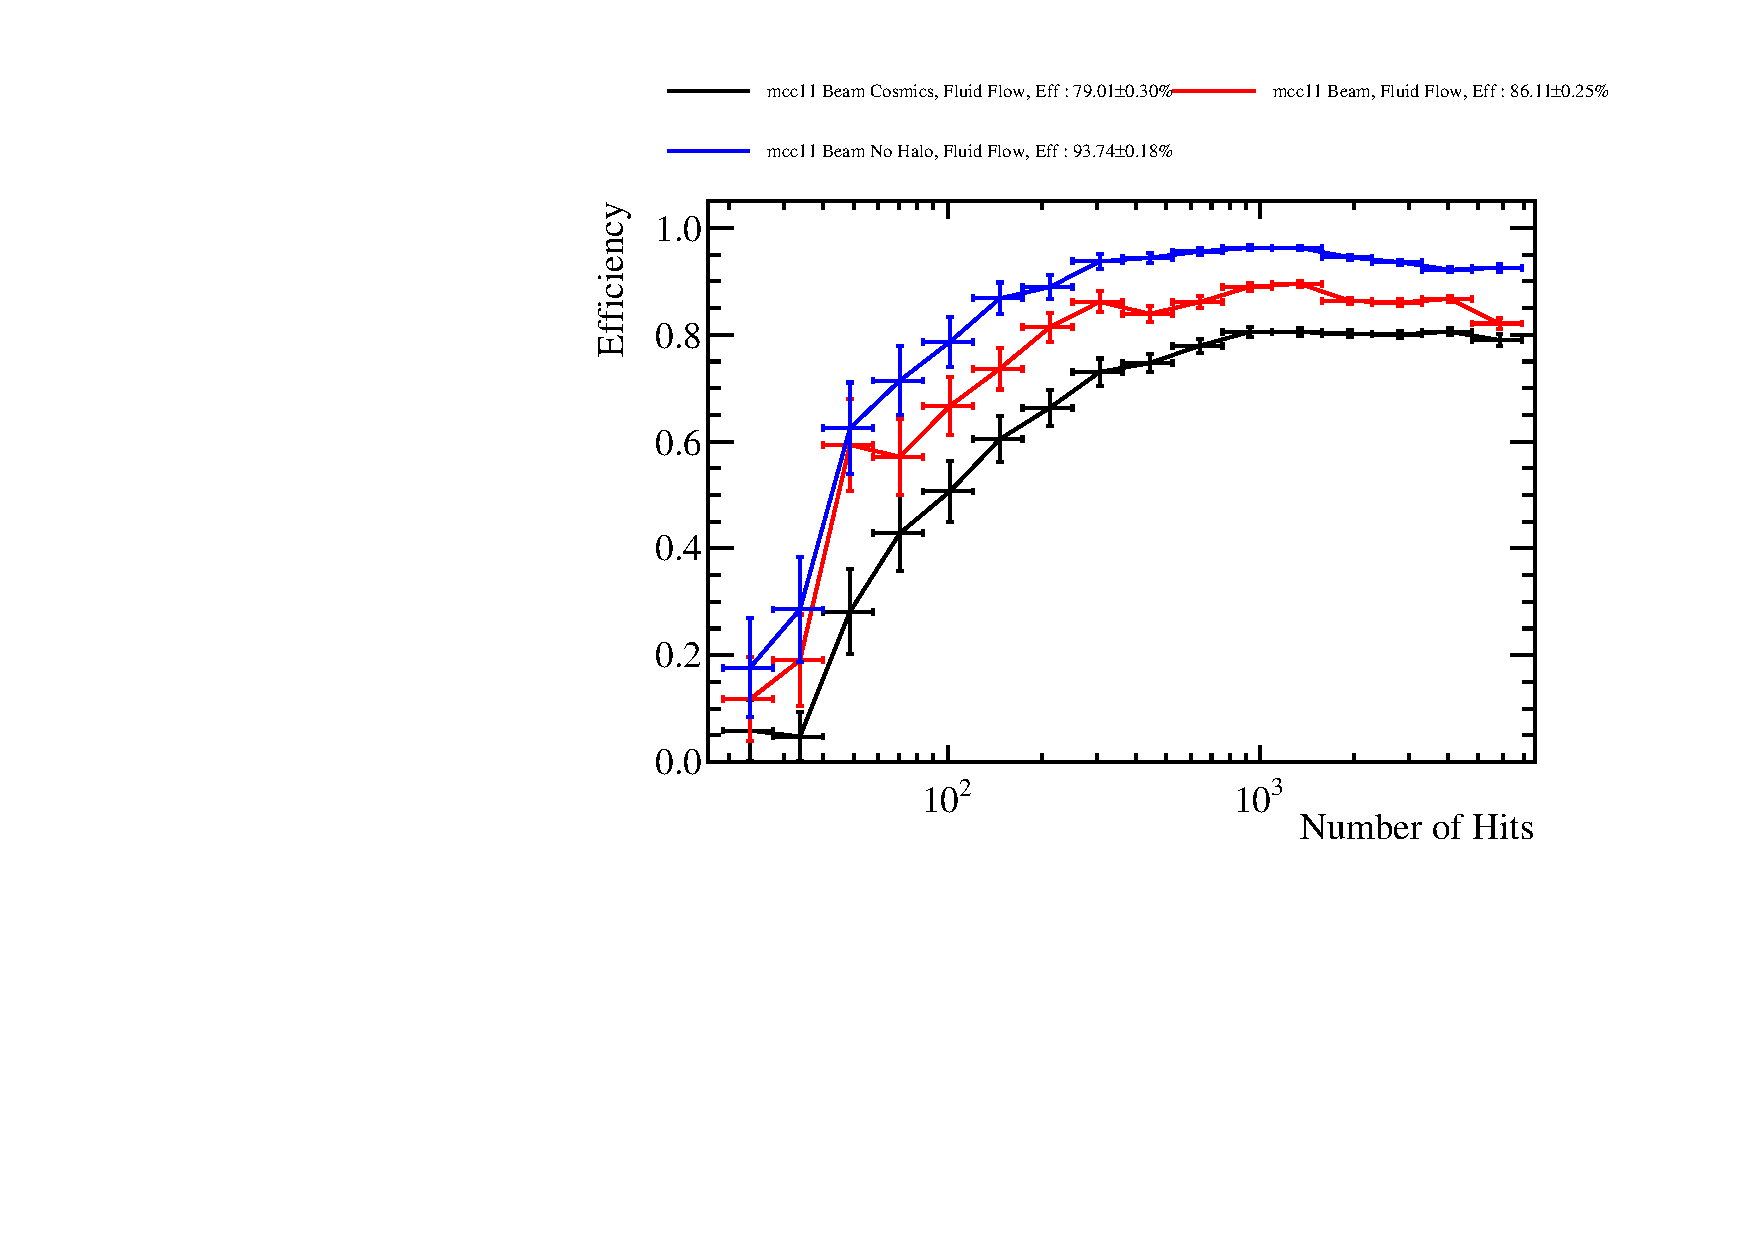
\includegraphics[width=0.45\textwidth]{Figures/Metrics/MC/Beam/Breakdown/BeamParticleEfficiencyBreakdownVsNHits.pdf}
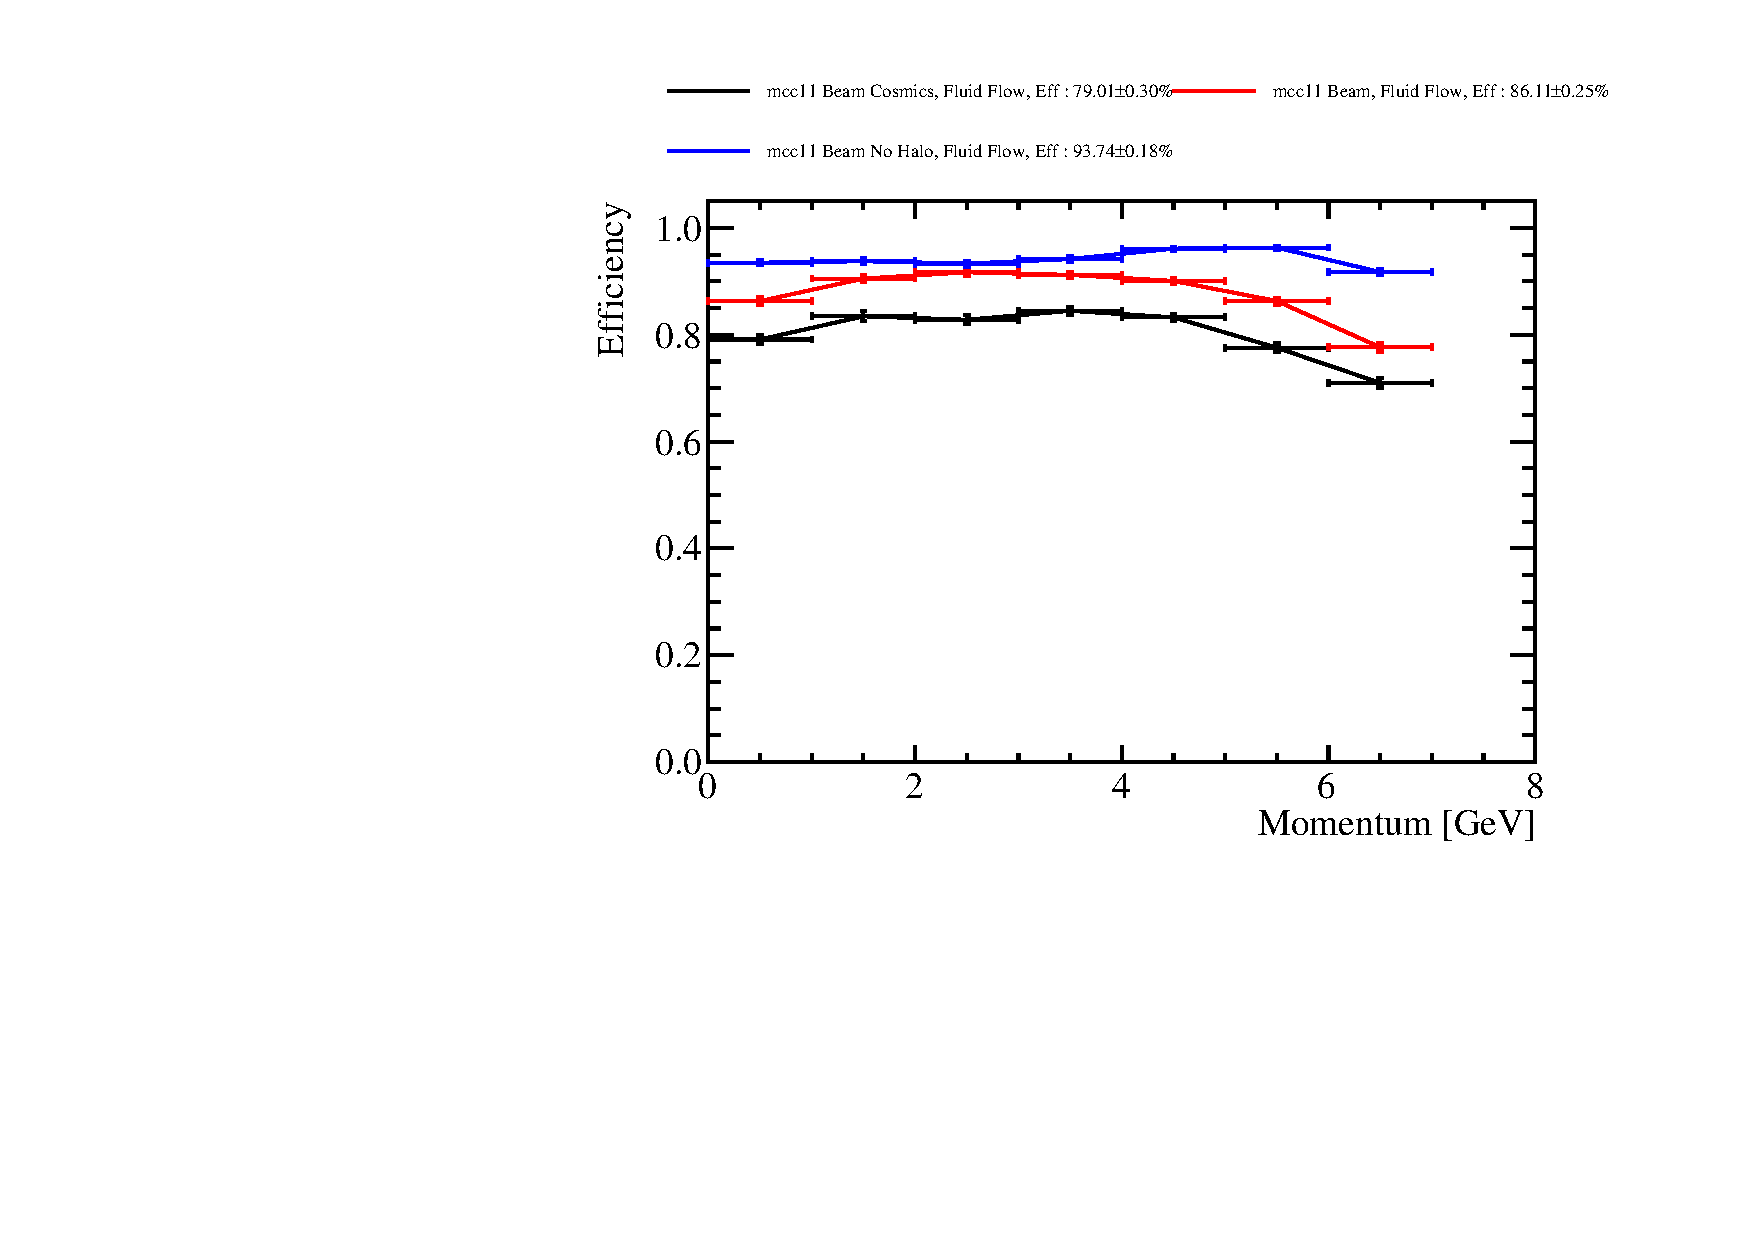
\includegraphics[width=0.45\textwidth]{Figures/Metrics/MC/Beam/Breakdown/BeamParticleEfficiencyBreakdownVsMomentum.pdf} \\
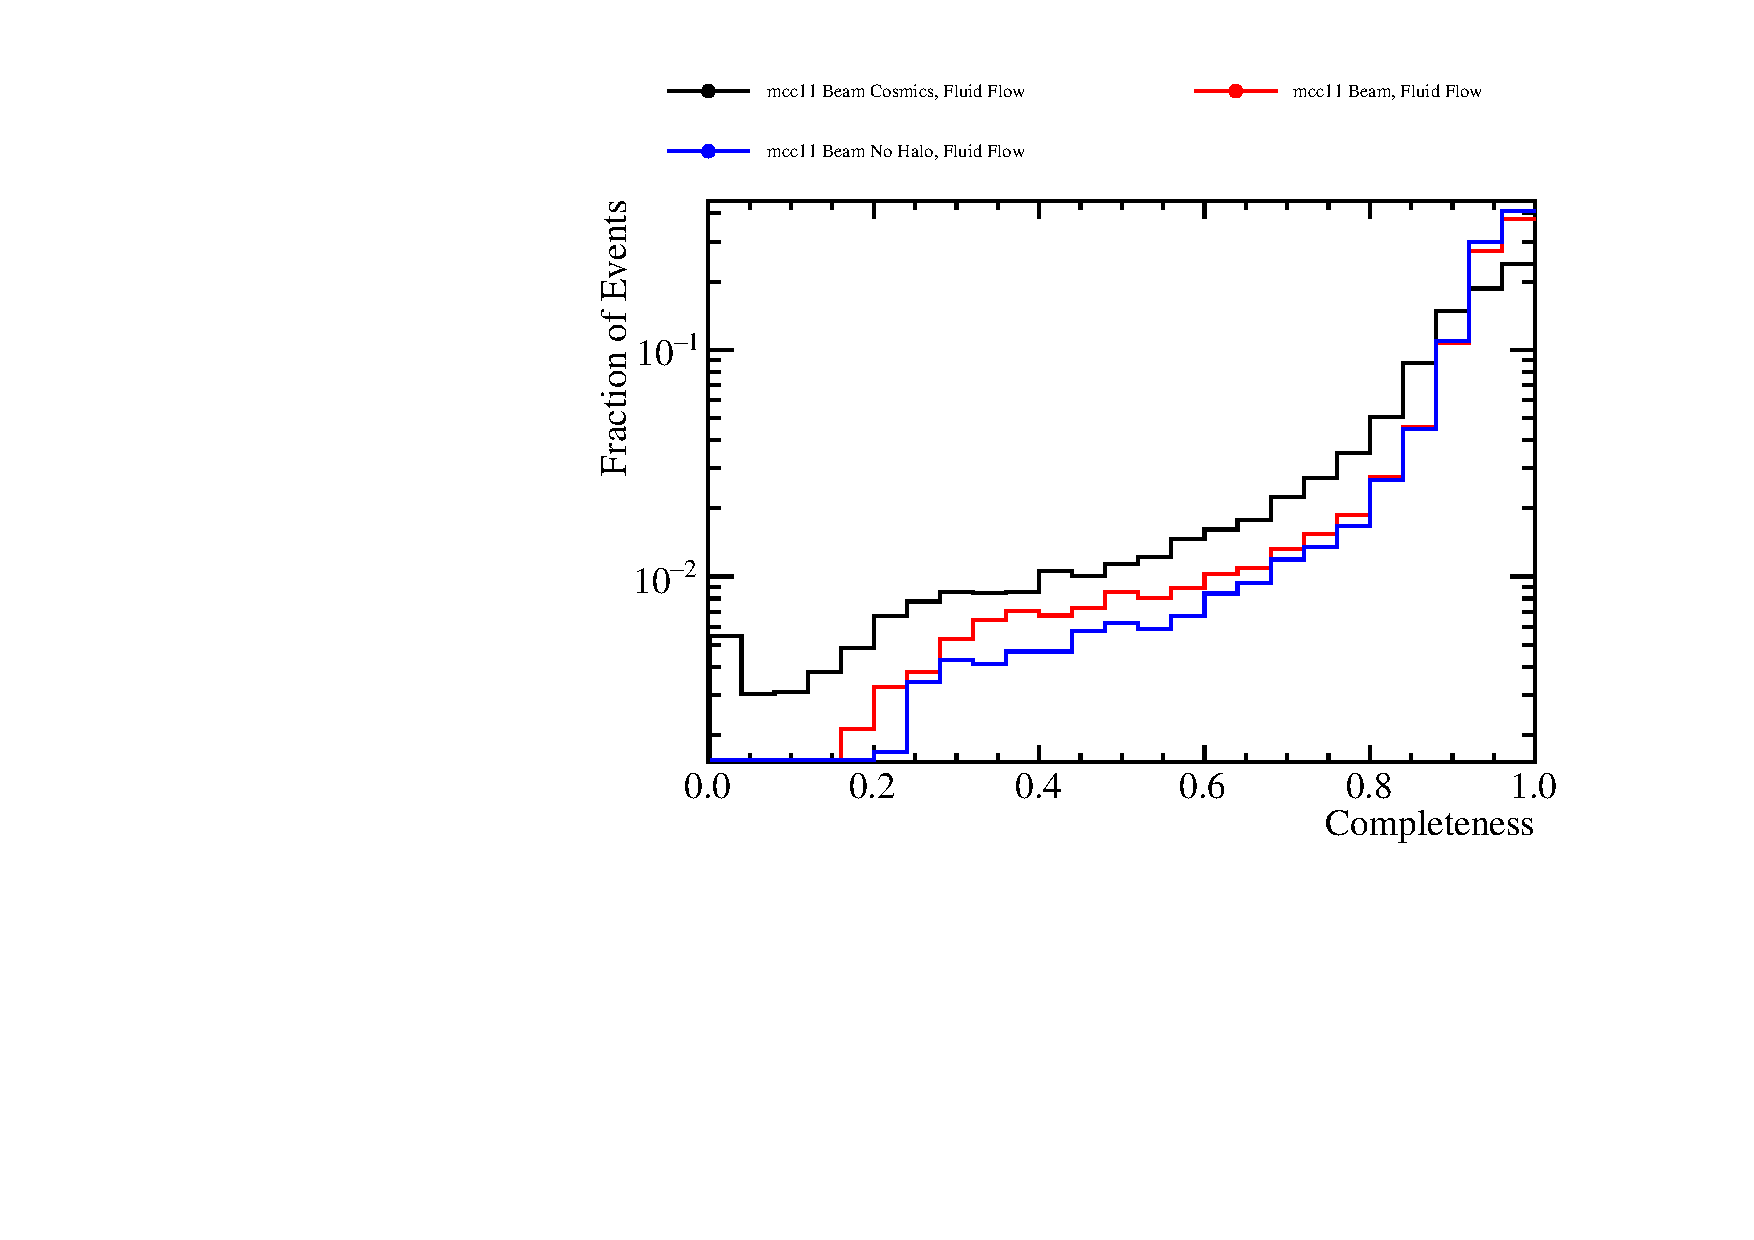
\includegraphics[width=0.45\textwidth]{Figures/Metrics/MC/Beam/Breakdown/BeamParticleCompleteness.pdf}
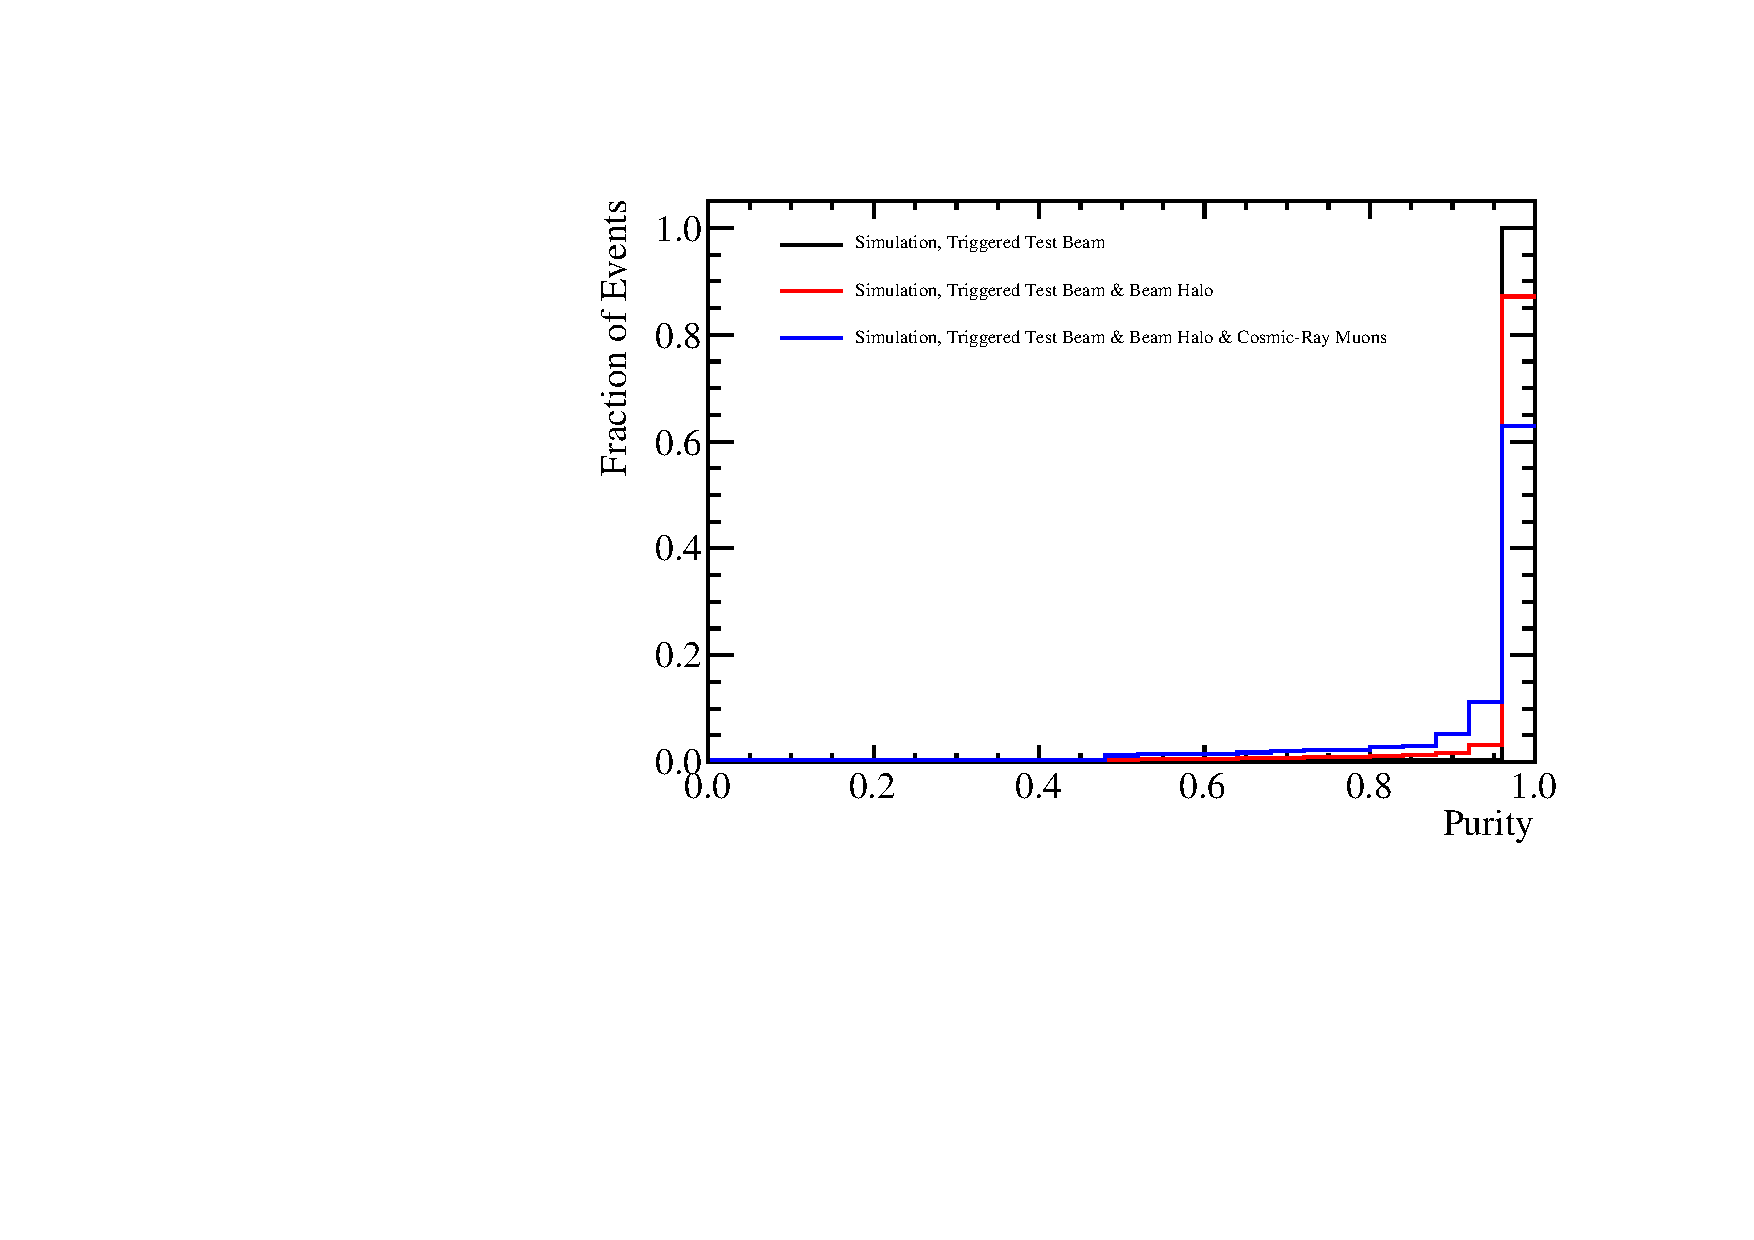
\includegraphics[width=0.45\textwidth]{Figures/Metrics/MC/Beam/Breakdown/BeamParticlePurity.pdf}
\caption{The test beam particle reconstruction efficiency metric when removing cosmic rays and beam halo.}
\label{fig:tbrecoeffbrkdwn}
\end{figure}

\begin{table}
\centering
\caption{The reconstruction efficiency for the test beam particle in MC as a function of beam momenta.}
\label{tab:1} 
\begin{tabular}{cc}
\hline\noalign{\smallskip}
Beam Momenta [GeV] & Reconstructed Efficiency  \\
\noalign{\smallskip}\hline\noalign{\smallskip}
1 & 87.5$\pm$0.8 \\
2 & 91.0$\pm$0.7 \\
3 & 92.7$\pm$0.6 \\
4 & 89.8$\pm$0.5 \\
5 & 89.0$\pm$0.5 \\
6 & 82.1$\pm$0.7 \\
7 & 75.4$\pm$0.7 \\
\noalign{\smallskip}\hline
\end{tabular}
\end{table}

\subsubsection{Cosmic Ray Metrics}
\label{sec:crmetrics}
Figure \ref{fig:crrecoeff} shows the reconstruction efficiency for cosmic rays as a function of the number of hits in the detector, which yields an integrated efficiency of 95\%.  The purity and completeness of the reconstructed cosmic rays are shown in figure \ref{fig:crrecopurcom}, both of which show strong peaks at 1.

\begin{figure}
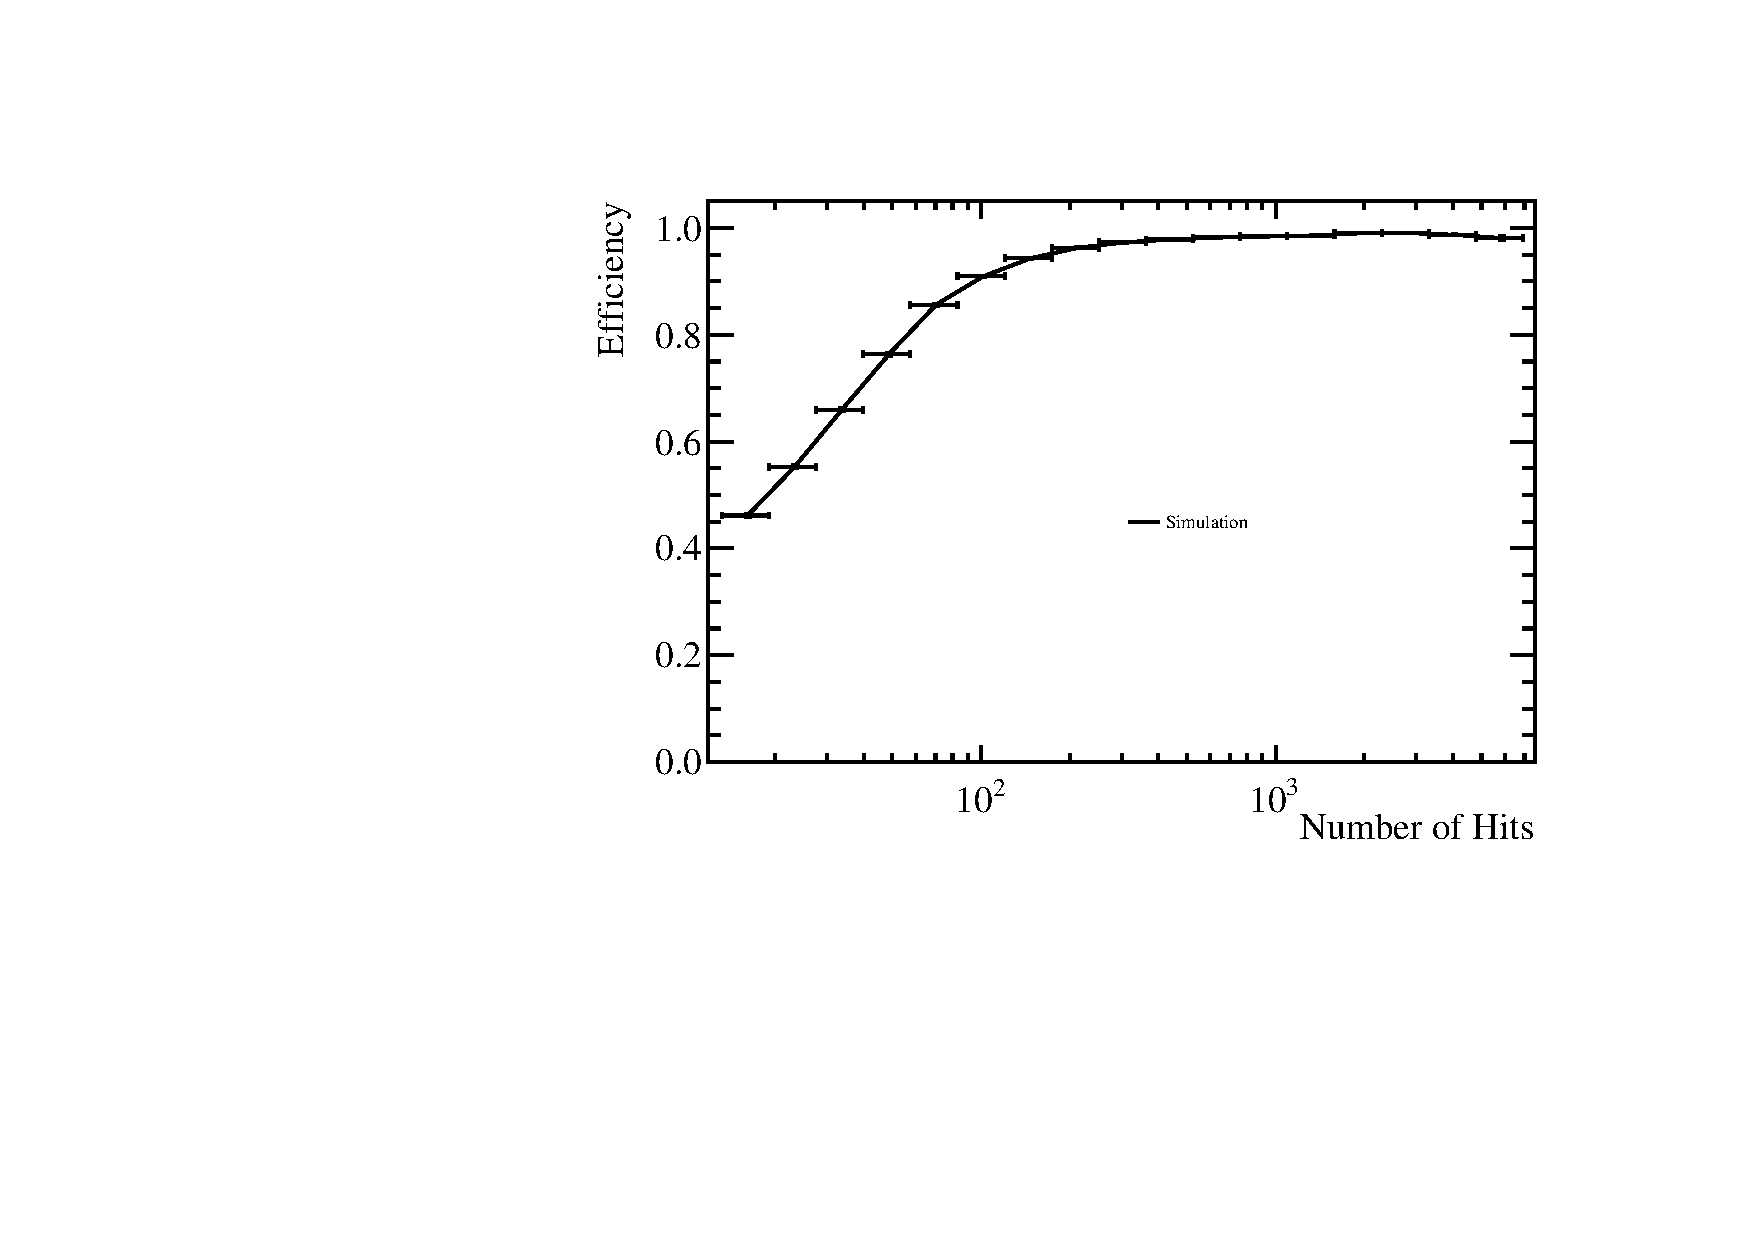
\includegraphics[width=0.75\textwidth]{Figures/Metrics/MC/Cosmics/CosmicRayEfficiencyVsNHits.pdf}
\caption{The reconstruction efficiency for cosmic rays in MC as a function of number of hits.}
\label{fig:crrecoeff}
\end{figure}

\begin{figure}
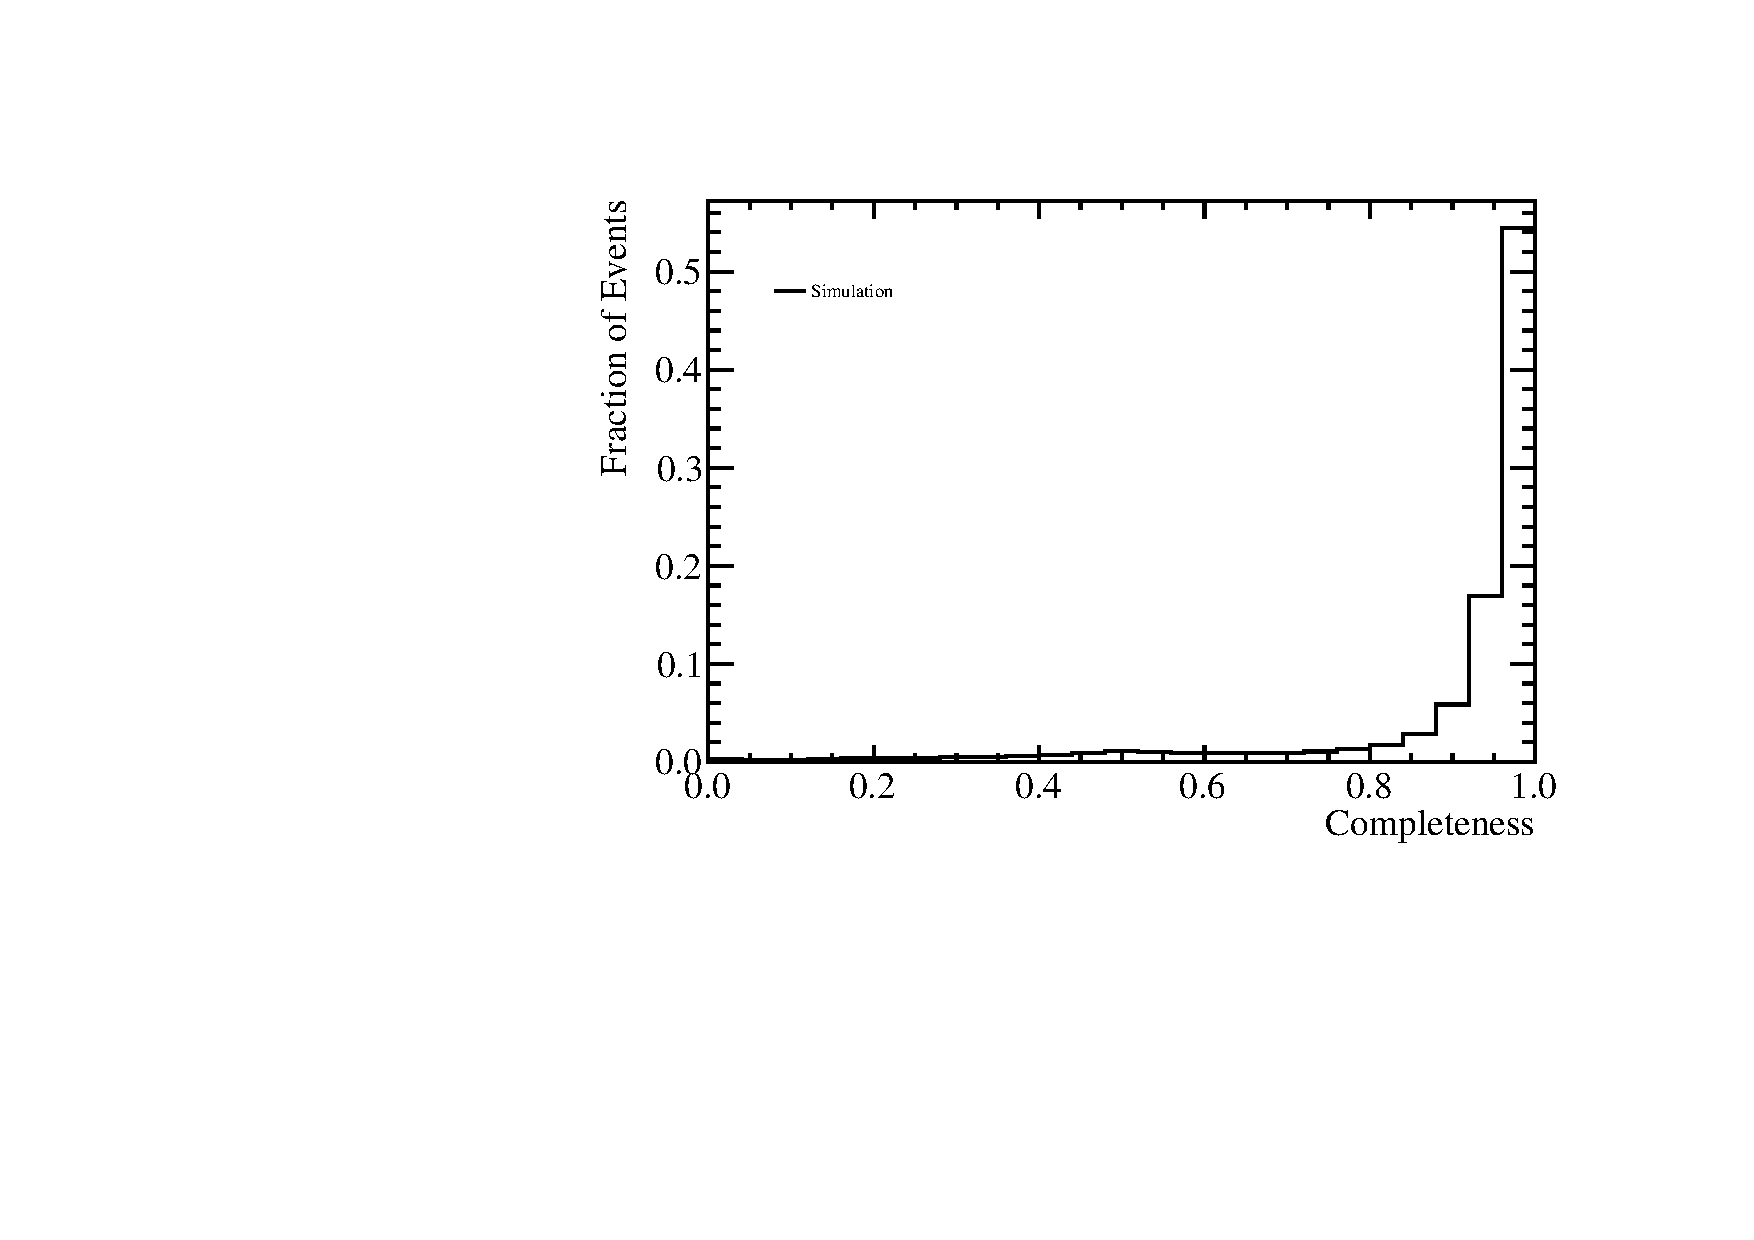
\includegraphics[width=0.5\textwidth]{Figures/Metrics/MC/Cosmics/CosmicRayCompleteness.pdf}
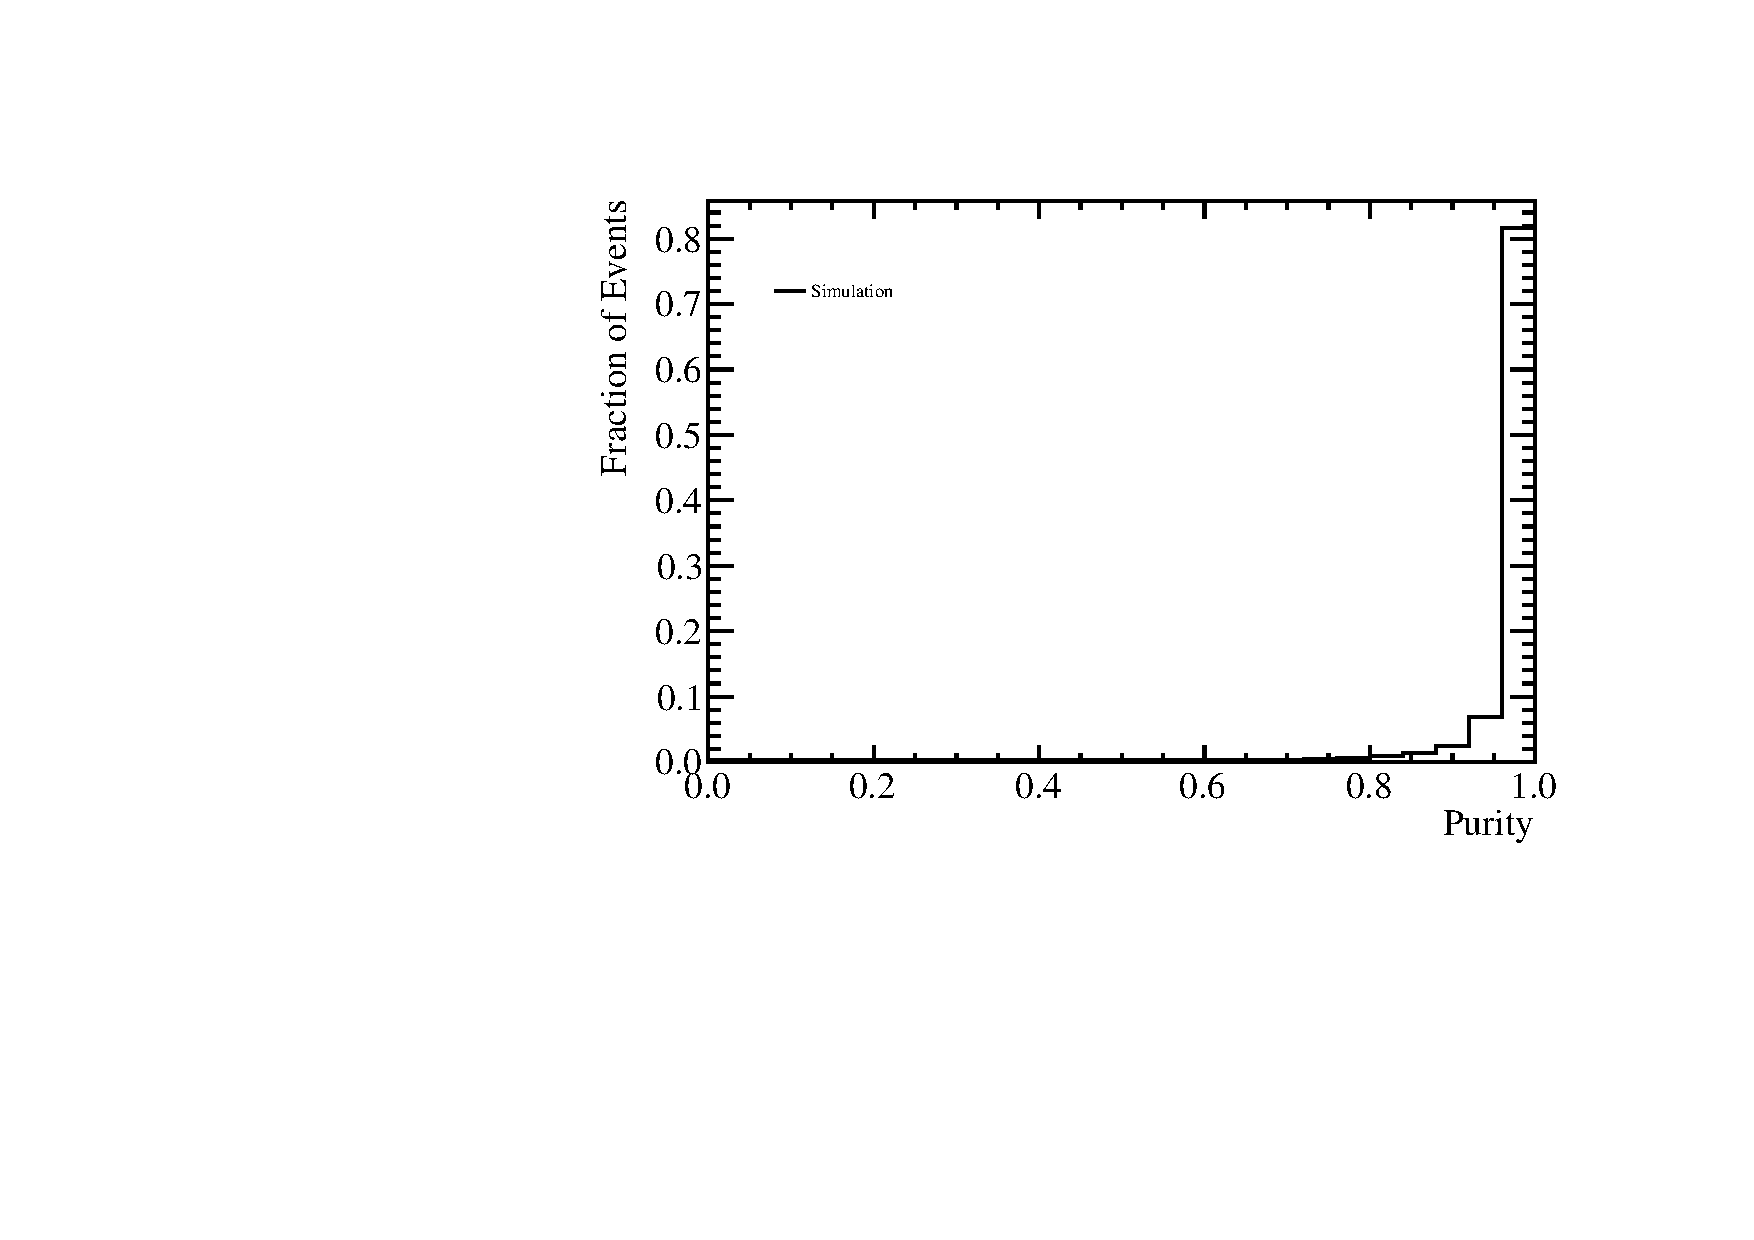
\includegraphics[width=0.5\textwidth]{Figures/Metrics/MC/Cosmics/CosmicRayPurity.pdf}
\caption{The purity and completeness of reconstructed cosmic ray particles in MC.}
\label{fig:crrecopurcom}
\end{figure}

It is also possible to tag the true $T_{0}$ of reconstructed cosmic rays if they are stitched by the processed discussed in section \ref{sec:consolidatedreco}.  The distribution of the resolution of the reconstructed $T_{0}$ for cosmic rays is shown in figure \ref{fig:crt0res}.  As expected, the impact of space charge in the simulation leads to a degradation in the $T_{0}$ resolution and the addition of the fluid flow model, which includes asymmetric space charge effects, leads to further degradation.  

\begin{figure}
\centering
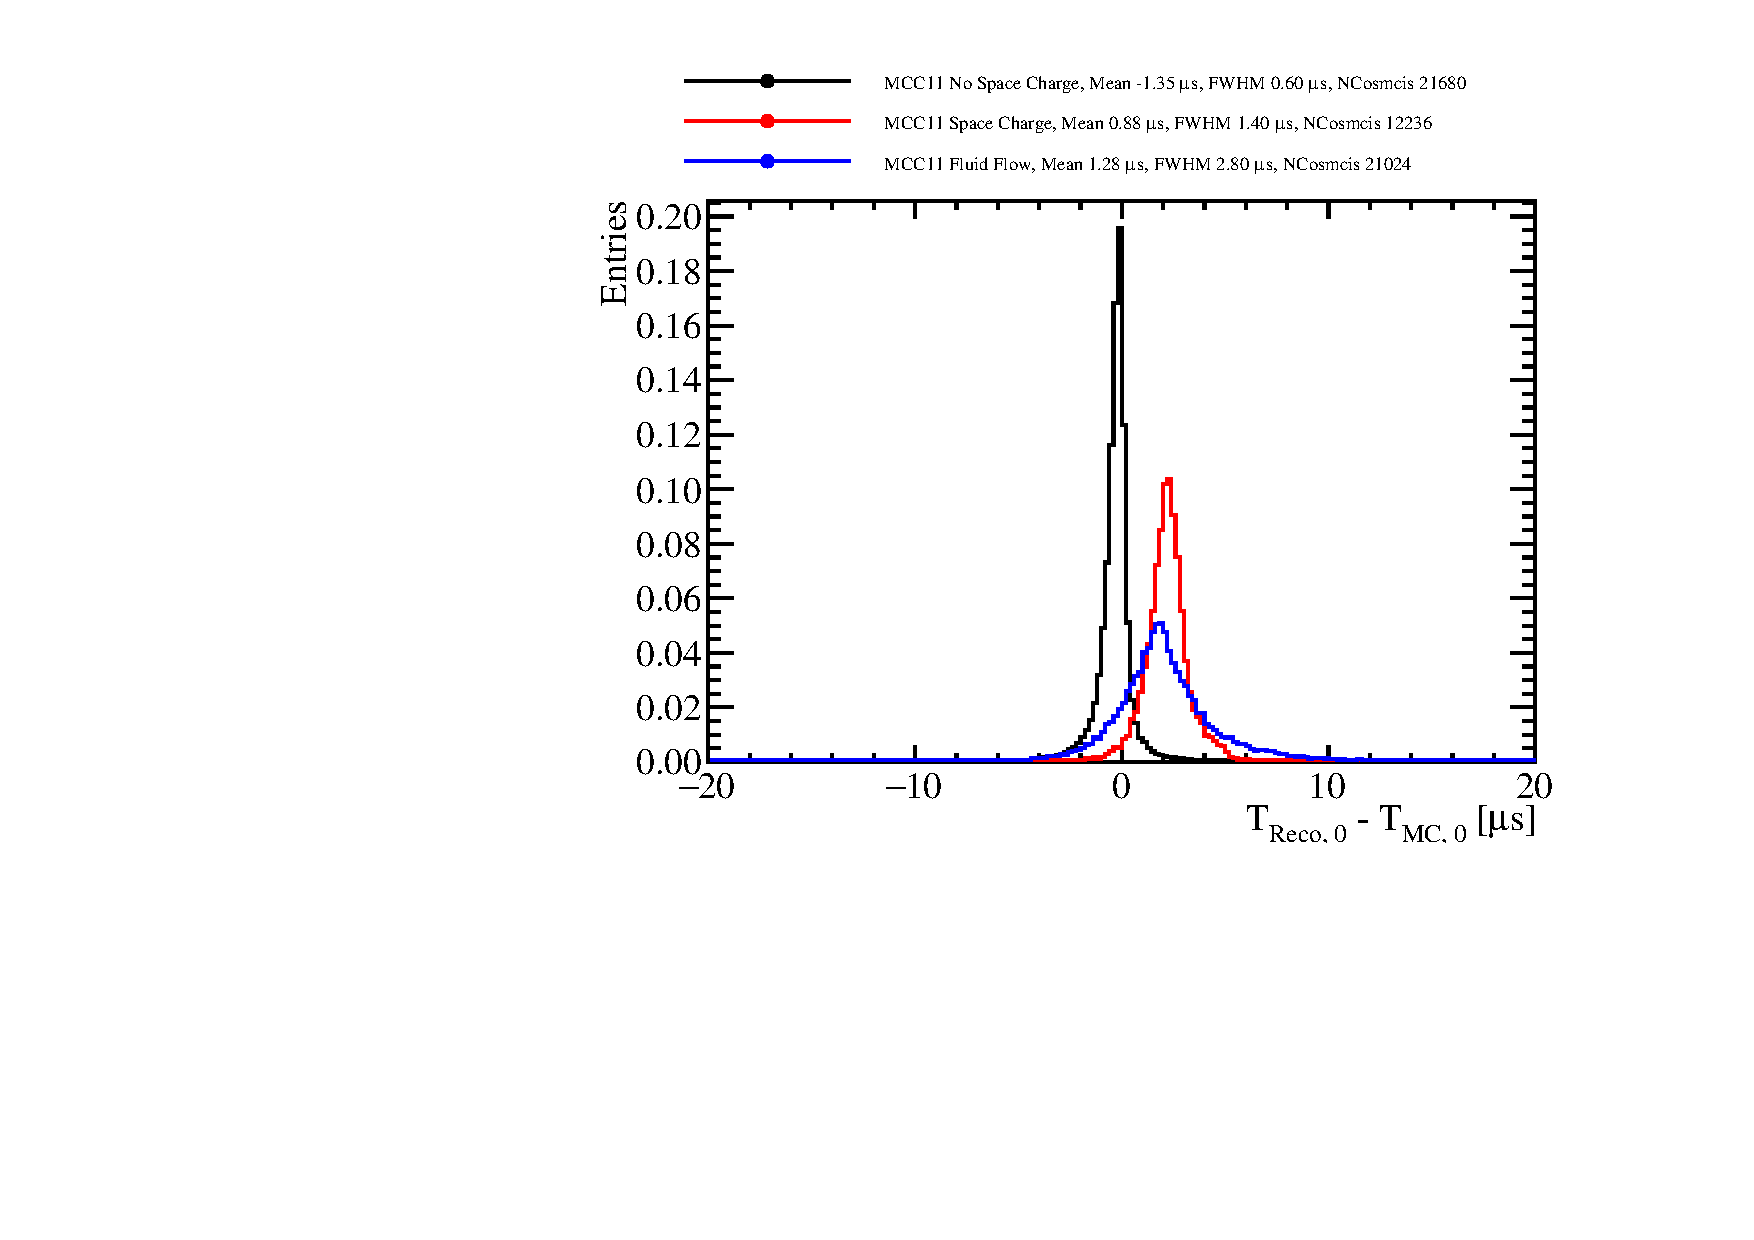
\includegraphics[width=0.75\textwidth]{Figures/Metrics/MC/Cosmics/CosmicRayT0Resolustion.pdf}
\caption{The resolution on the reconstructed $T_{0}$ for cosmic rays in MC.}
\label{fig:crt0res}
\end{figure}

In order to give context to the topologies that the reconstruction is faced with at ProtoDUNE-SP an estimate of the number of cosmic rays passing through the detector per event.  The number of reconstructed cosmic rays matched to clear cosmic rays, i.e. depositing more than 100 hits in the detector, is shown as a function of the number of clear cosmic rays in figure \ref{fig:crnperevt}.  This shows that, on a per event basis, the reconstruction is predominantly working on the reconstruction of cosmic rays.

\begin{figure}
\centering
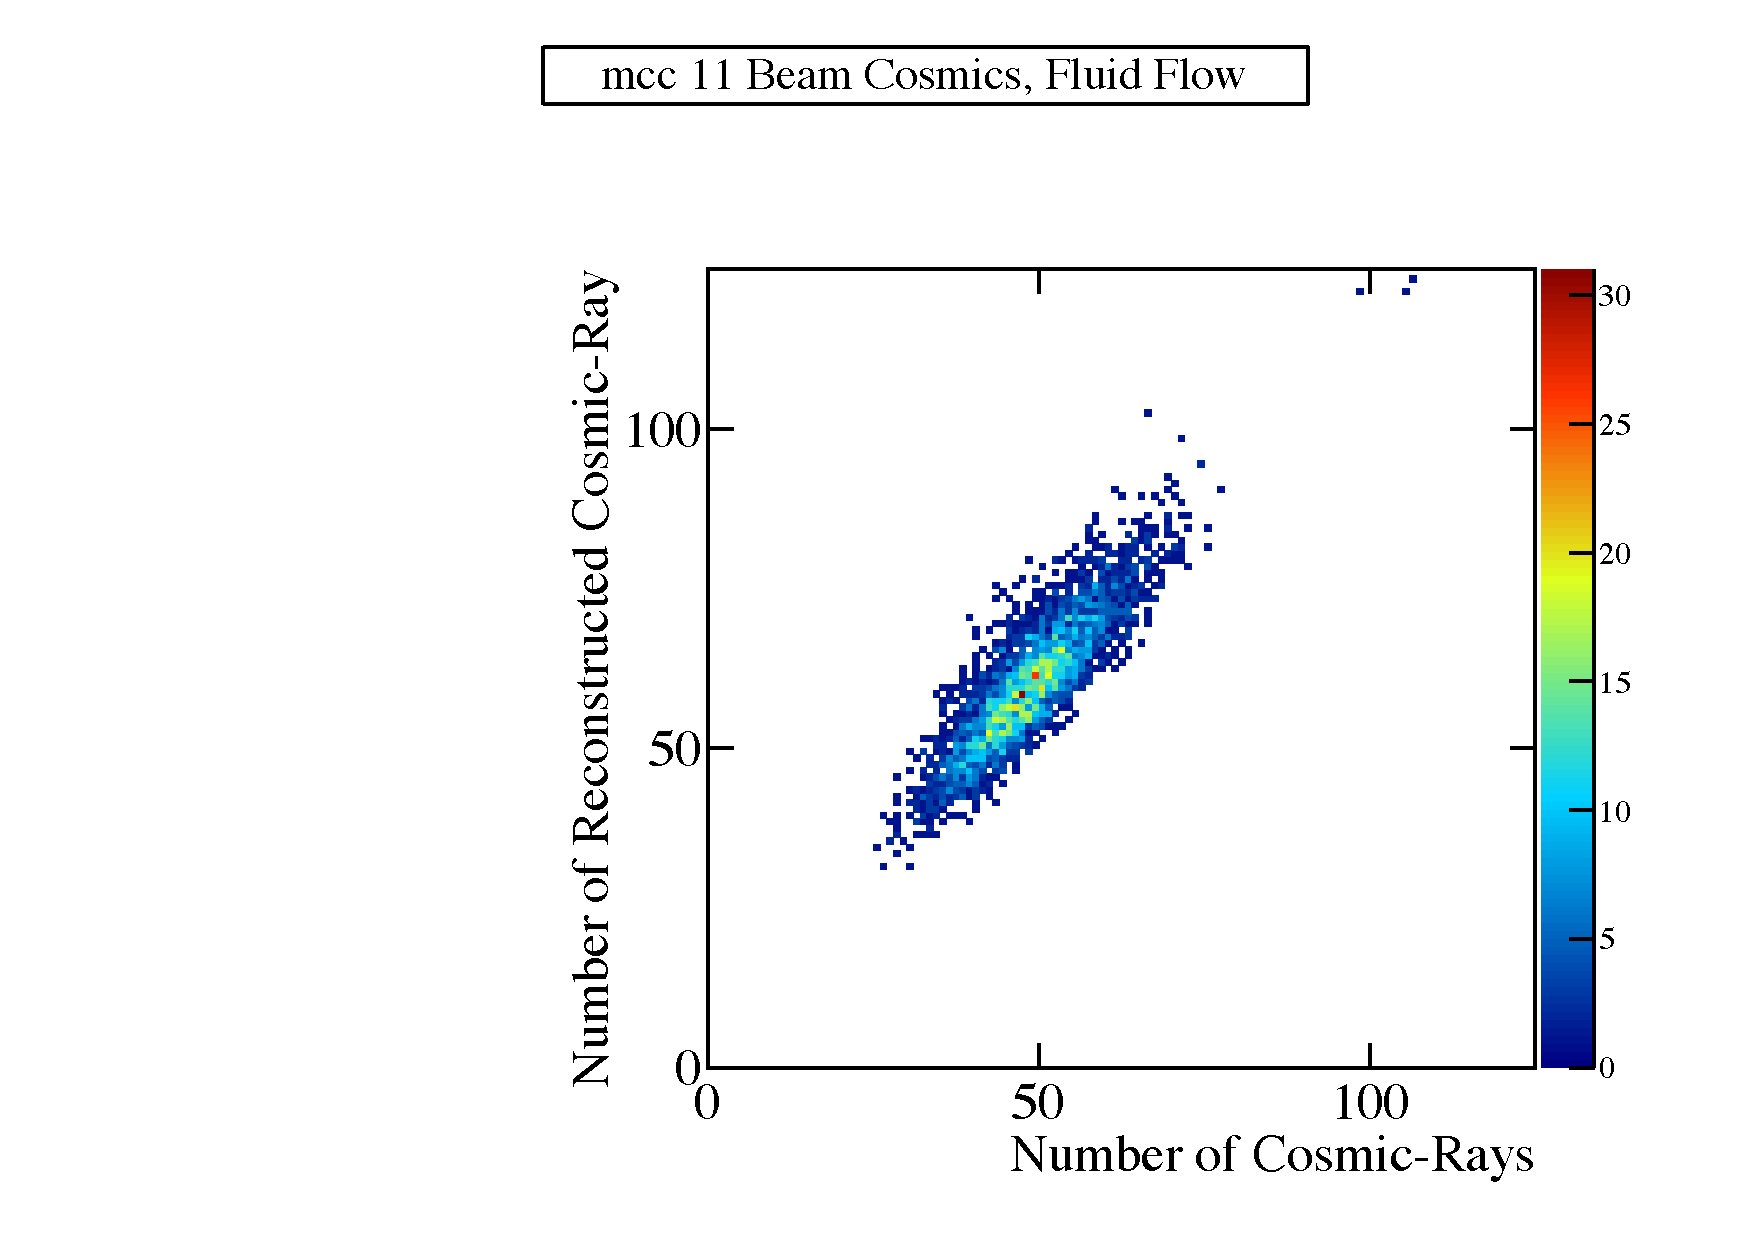
\includegraphics[width=0.75\textwidth]{Figures/Metrics/MC/Cosmics/CRMatchesCosmicRayEvent.pdf}
\caption{The number of matched reconstructed cosmic rays per event as a function of the true number of cosmic rays for cosmic rays depositing more than 100 hits in the detector.  The cut at 100 hits allows a clearer comparison to be made to data in subsequent studies due to the higher reconstruction efficiency for these cosmic rays with respect to those depositing less than 100 hits.}
\label{fig:crnperevt}
\end{figure}

\subsection{Data}

ProtoDUNE took test beam data at CENR between October and December 2018.  What follows is a flavour of how the Monte-Carlo metrics discussed above compare to data.  This data presents the Pandora reconstruction with several unique challenges that have not been seen at other active LArTPC experiments, such as stitching of cosmic rays due to the presence of multiple drift volumes is possible and the reconstruction is that of test beam particles not neutrinos.  

\subsubsection{Test Beam Metrics}

A crucial metric describing the performance of the pattern recognition at ProtoDUNE-SP is the triggered test beam particle reconstruction efficiency.  This metric folds in effects from each step of the reconstruction procedure and crucially the test beam particle id step.  In order for a reconstructed event to be counted as efficient, a reconstructed object must be classified as originating from the test beam.  As access to the underlying truth information for data is not possible, the reconstruction metric used for this data MC comparison does not use the matching procedure described in section \ref{sec:mcmetrics}.  Instead an event is deemed efficient when for:

\begin{itemize}
    \item \textbf{Data} The trigger is active and indicates the presence of a single particle and there is a reconstructed test beam particle in the event output.
    \item \textbf{Monte-Carlo} There is a triggered test beam particle in the MC particle hierarchy and there is a reconstructed test beam particle in the event output.
\end{itemize}

The reconstruction efficiency for ProtoDUNE for separate beam momentum runs is shown in table \ref{tab:dataeff}.  

\begin{table}
\centering
\caption{The reconstruction efficiency for the test beam particle in data as a function of beam momenta.}
\label{tab:dataeff} 
\begin{tabular}{cc}
\hline\noalign{\smallskip}
Beam Momenta [GeV] & Reconstructed Efficiency  \\
\noalign{\smallskip}\hline\noalign{\smallskip}
1 & 70.6$\pm$0.3 \\
2 & 84.2$\pm$0.3 \\
3 & 86.8$\pm$0.2 \\
6 & 85.2$\pm$0.2 \\
7 & 83.7$\pm$0.2 \\
\noalign{\smallskip}\hline
\end{tabular}
\end{table}

The ProtoDUNE trigger also measures the momentum of the triggered test beam particle, therefore the reconstruction efficiency is plotted as a function of the triggered test beam particle momentum in figure \ref{fig:datamcrecoeff}.  

\begin{figure}
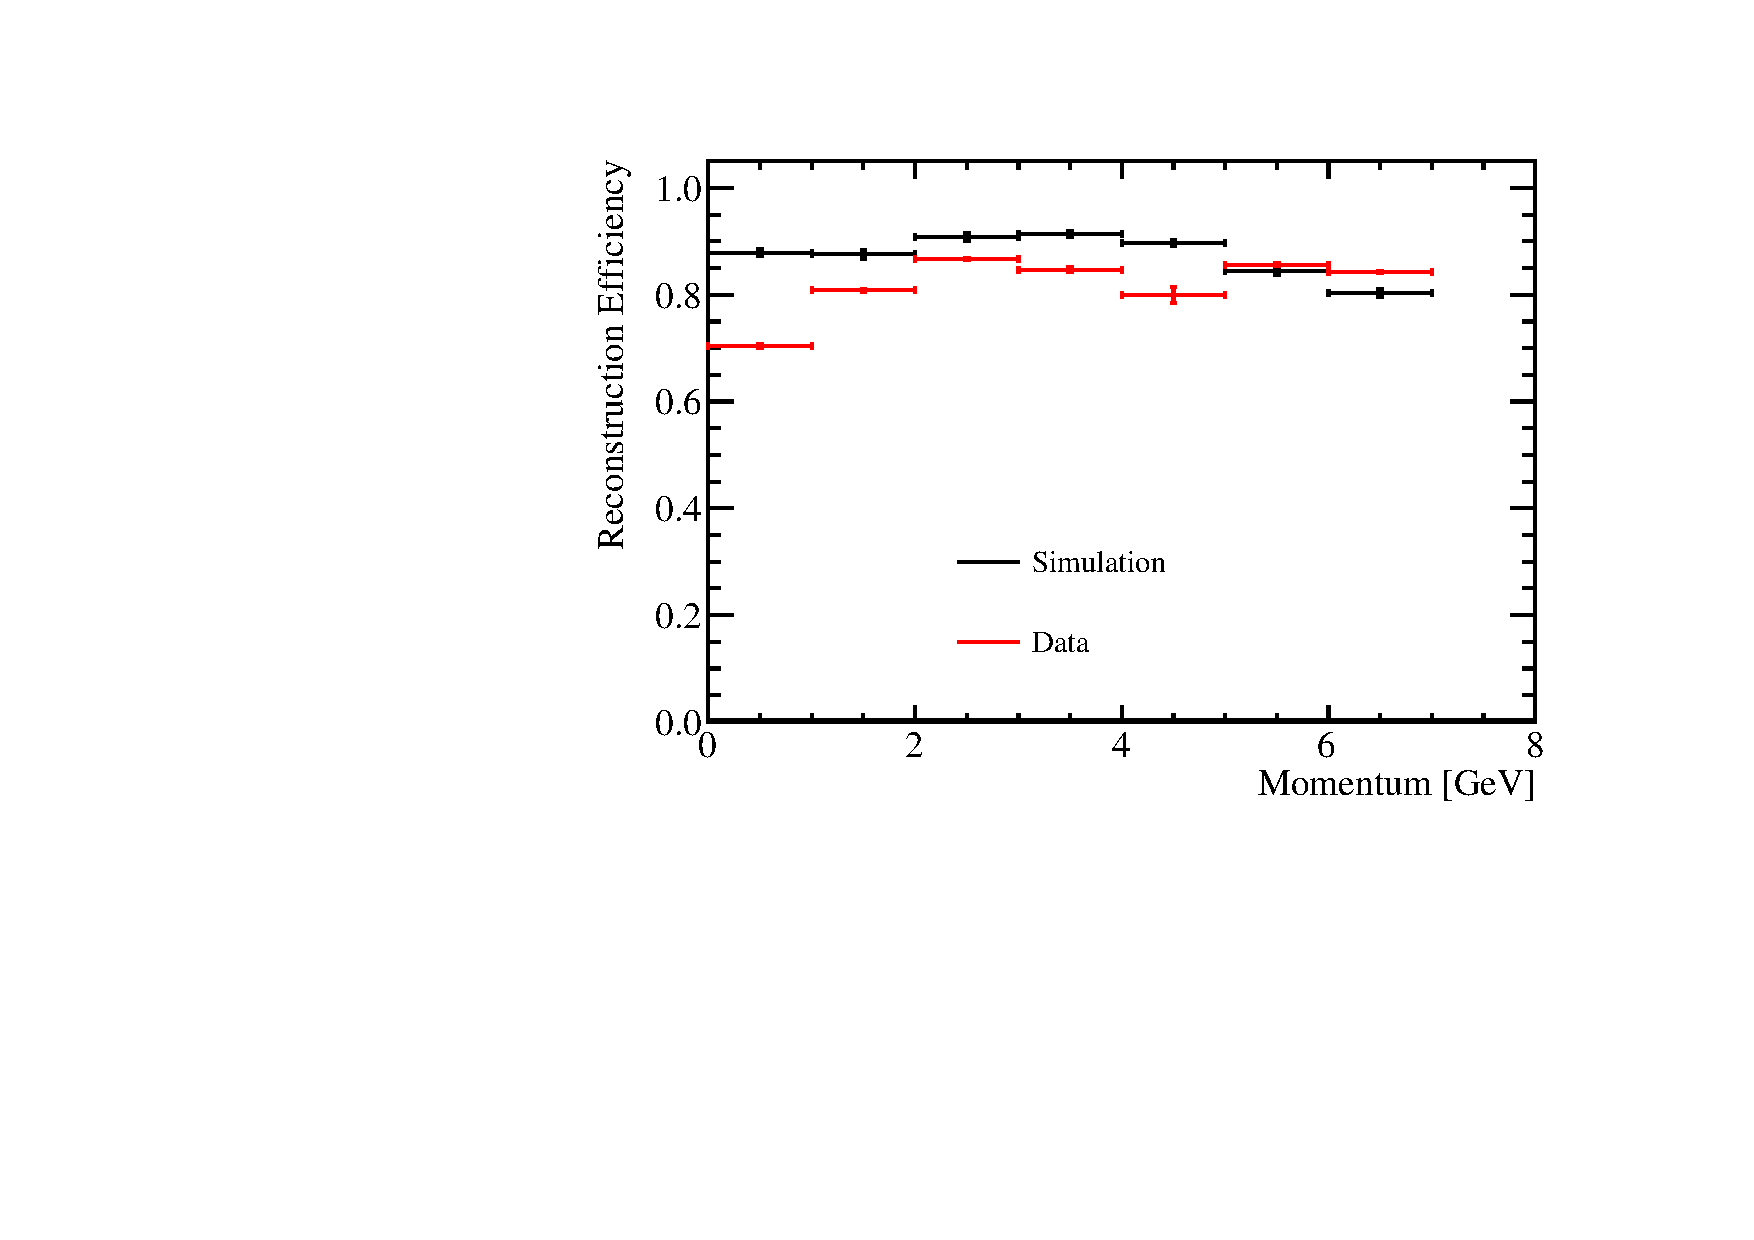
\includegraphics[width=1.0\textwidth]{Figures/Metrics/Data/Beam/BeamParticleEfficiencyVsMomentum.pdf}
\caption{The test beam particle reconstruction efficiency as a function of the number of hits in the test beam particle and the test beam particle momentum.}
\label{fig:datamcrecoeff}
\end{figure}

Overall, there is a typically good agreement between the reconstruction efficiency for data and MC with integrated efficiencies of ~80\% and \%80 respectively.  As a function of momentum, additional features are present.  In particular, at low momentum, where the reconstruction efficiency for data is lower than MC, and high momentum, where the reconstruction efficiency is higher for data than MC.  The disparity at low momentum is due to the trigger being active for certain events, but no clear test beam particle appearing in the detector.  %Probably missing enough justification here  

For high momentum the disparity is due to an overestimation of the beam halo in the MC samples.  This is evident from figure \ref{fig:tbrecoeffbrkdwn}, which indicates that the impact of cosmic rays at high beam momenta is almost negligible, while the beam halo dominates in inefficiencies in the reconstruction efficiency.  
In addition to the reconstruction efficiency it is also possible to evaluate higher level metrics for the reconstructed test beam particle describing the quality of the reconstructed object.  For example figure \ref{fig:openingangles} shows the opening angle between the reconstructed and expected direction of the triggered test beam particle.  For data the trigger provides a measurement of the particle direction, while for MC truth information is used for comparison.  While differences are present it is encouraging that both of these distributions peak at low values of opening angle.  The same distributions divided into track and shower like triggered test beam particles are included.  The broader distribution for showers indicates that, as expected, estimation of the direction of a clean single track like 3D particle is more precise than the estimation of a more disperse shower like object.   

\begin{figure}
\subfloat[]{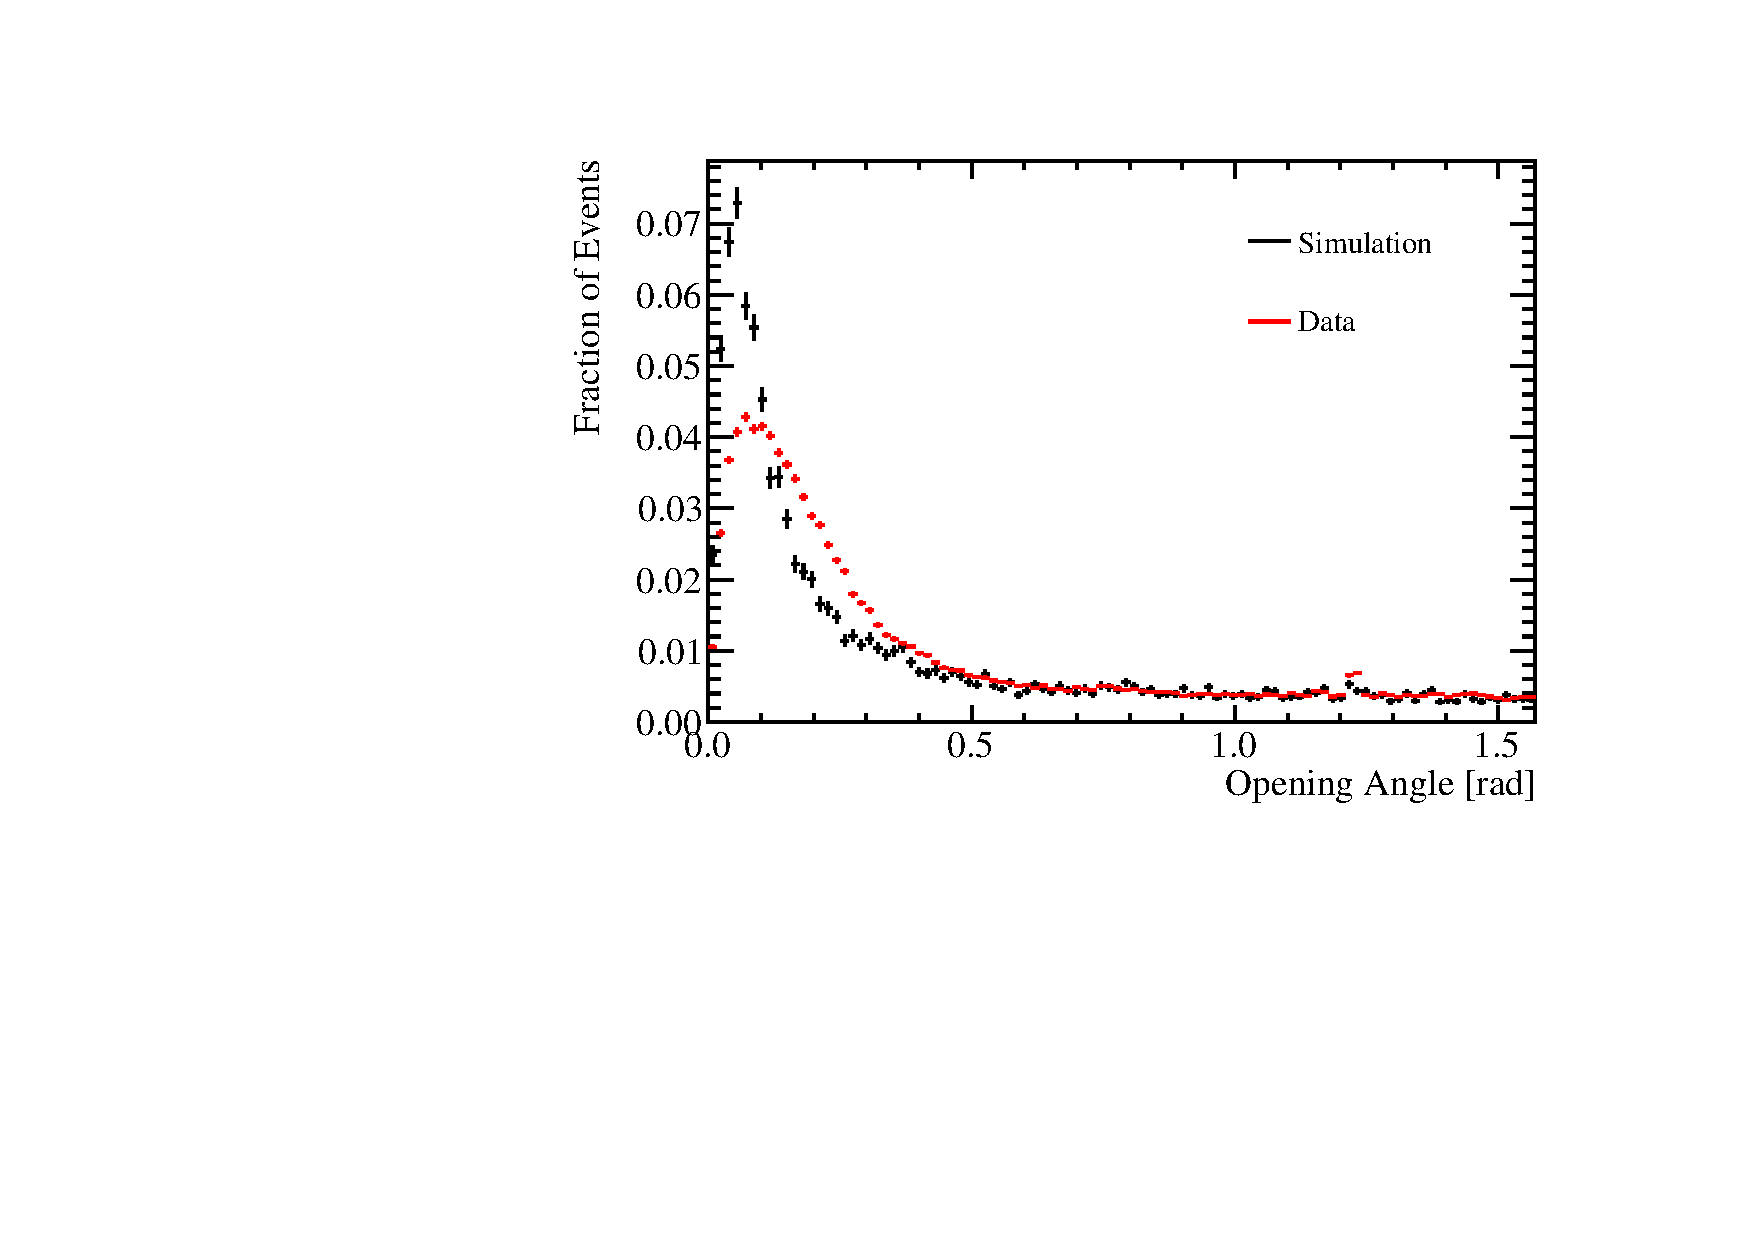
\includegraphics[width=1.0\textwidth]{Figures/Metrics/Data/Beam/BeamParticleOpeningAngle.pdf}\label{fig:openingangle}} \\
\subfloat[]{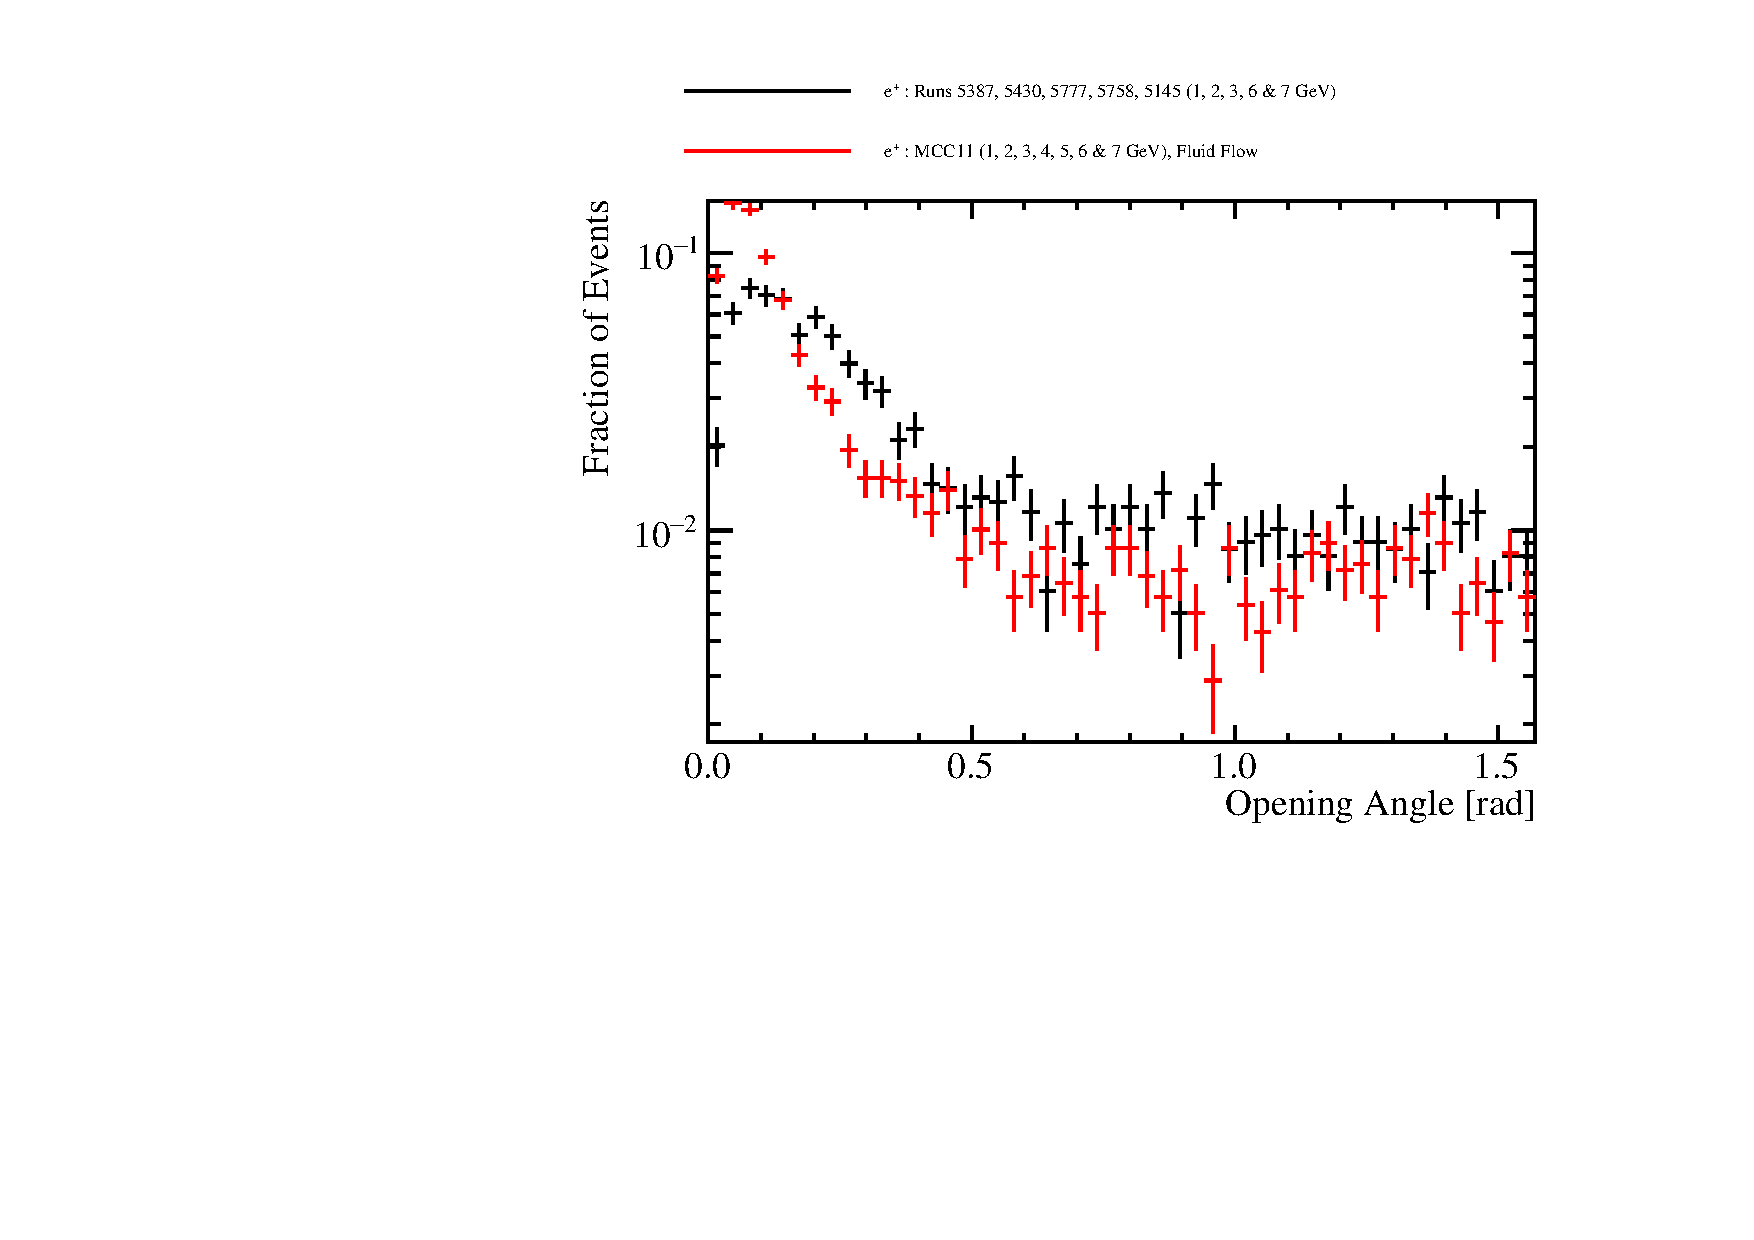
\includegraphics[width=0.5\textwidth]{Figures/Metrics/Data/Beam/BeamParticleOpeningAngleElectron.pdf}\label{fig:openingangleshw}}
\subfloat[]{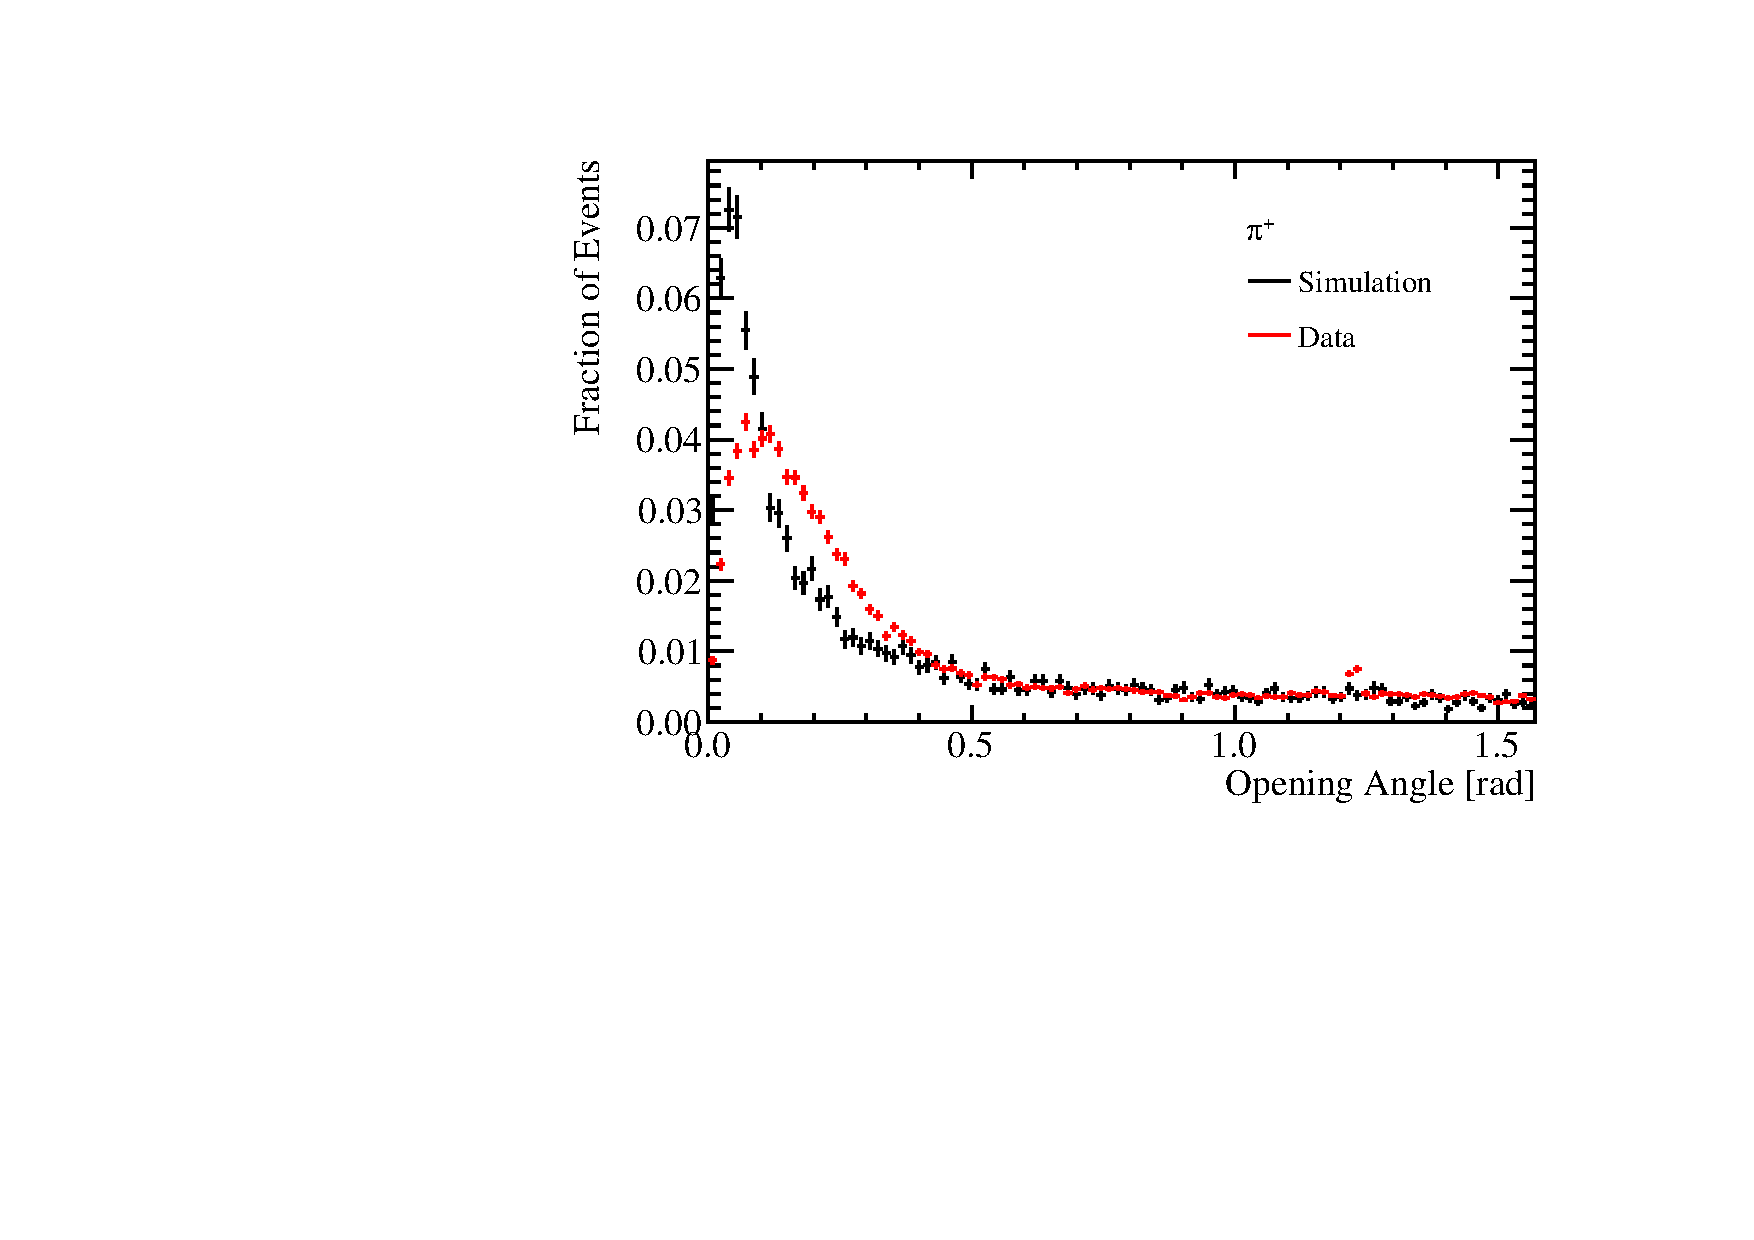
\includegraphics[width=0.5\textwidth]{Figures/Metrics/Data/Beam/BeamParticleOpeningAnglePiPlus.pdf}\label{fig:openingangletrk}}
\caption{\subref{fig:openingangle} The opening angle between a linear fit to the start of the reconstructed test beam particle as it enters the TPC and the MC truth direction direction.  \subref{fig:openingangleshw} and \subref{fig:openingangletrk} show the same distributions for $e^{+}$ and $\pi^{+}$ triggered particles only.}
\label{fig:openingangles}
\end{figure}

\subsubsection{Cosmic Ray Metrics}

Reconstruction metrics for reconstructed cosmic ray data have also been evaluated.  Figure \ref{fig:ncrdata} shows the number of reconstructed particles tagged as clear cosmic rays per event in ProtoDUNE.  For a cosmic ray to be tagged as clear it must deposit at least 100 hits in the detector.  This cut is applied in order to ensure a minimum reconstruction efficiency of ~90\%, based on the MC efficiencies in figure \ref{fig:crrecoeff}.  Therefore, this metric gives an accurate reflection of the true number of large cosmic rays in the detector.  

There is excellent agreement between data and MC in the number of clear cosmic rays per event, with both distributions peaking around 50 cosmic rays per event.  The width of both distributions is similar, however the MC distribution is slightly broader and contains a high tail indicating that the MC flux is slightly overestimated in simulation.  

\begin{figure}
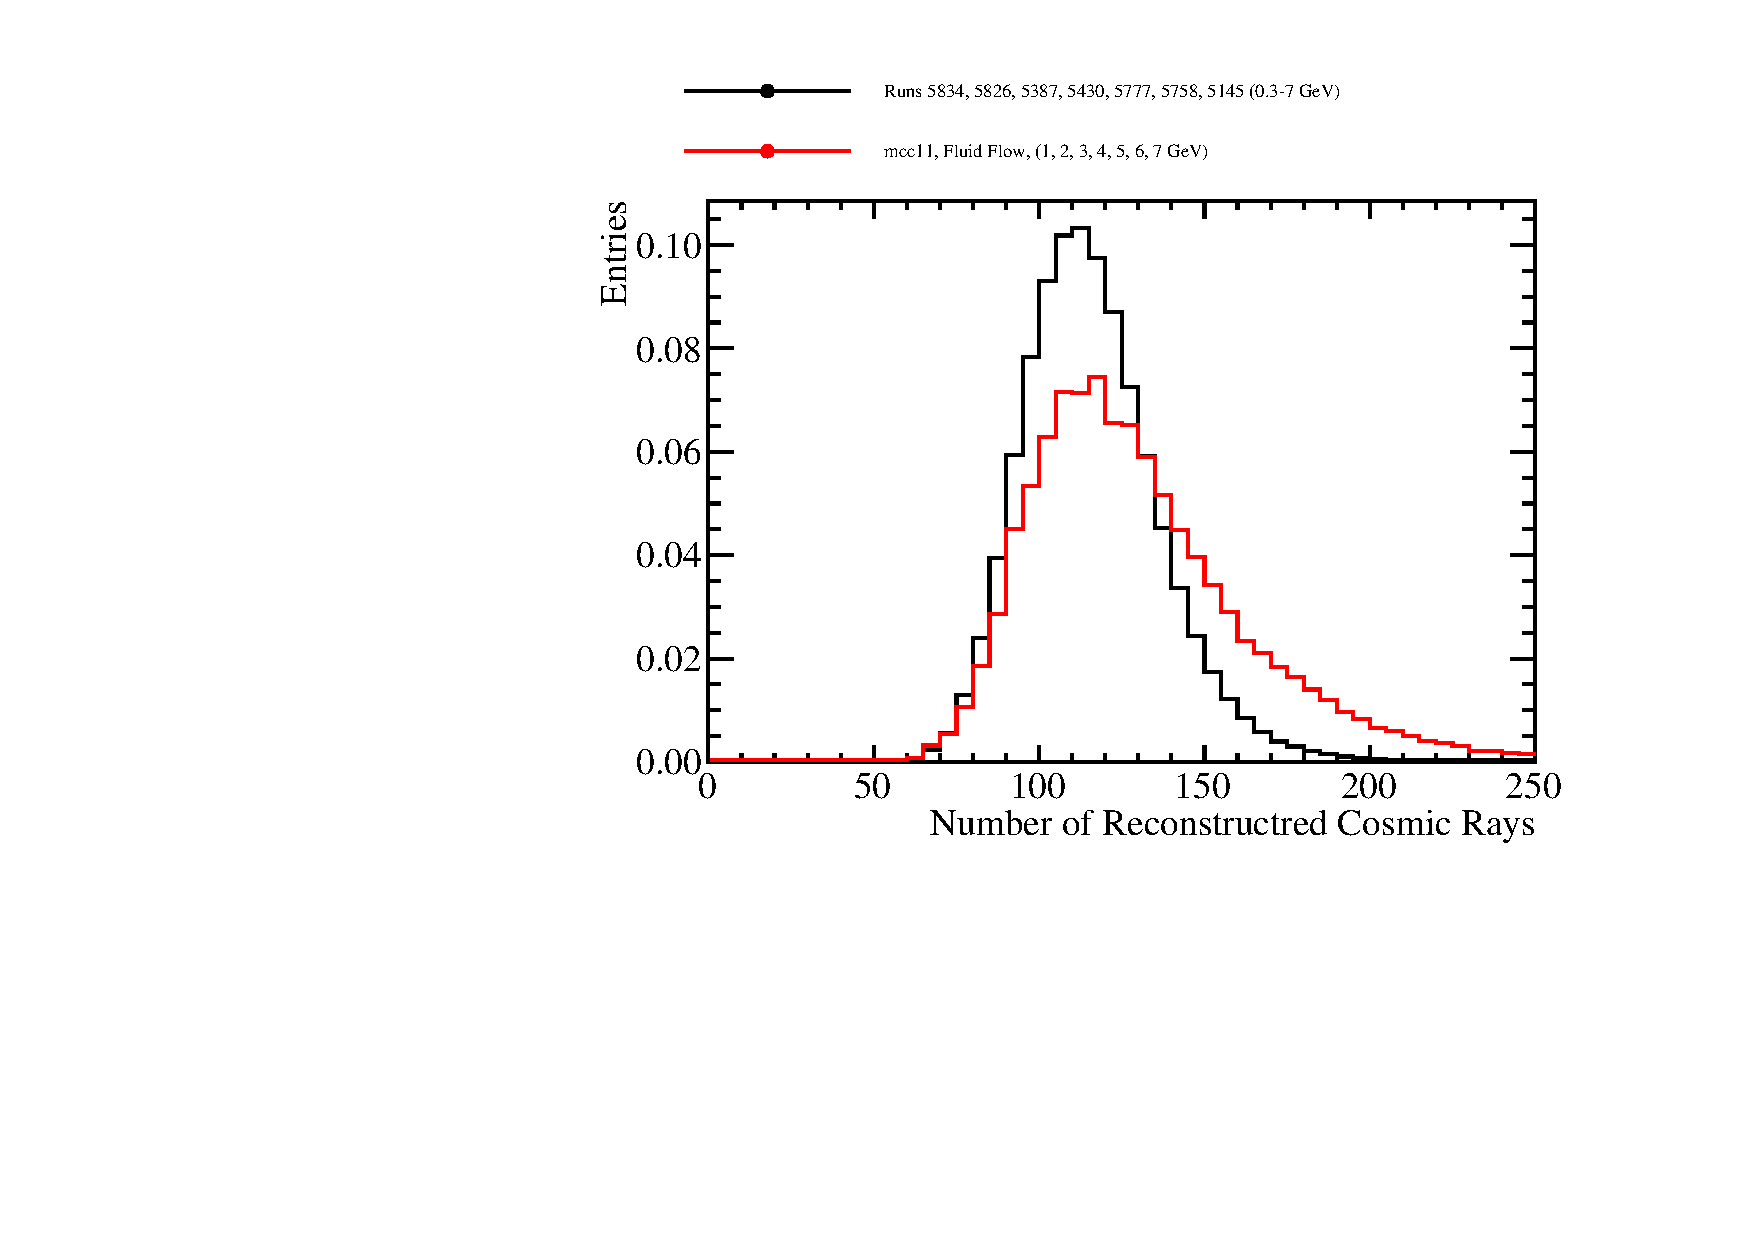
\includegraphics[width=1.0\textwidth]{Figures/Metrics/Data/Cosmics/NumberofReconstructedCosmicRays.pdf}
\caption{The number of reconstructed clear cosmic ray particles per event.  A reconstructed particle is classified as a clear cosmic ray if it has been reconstructed and tagged as a cosmic ray and has deposited at least 100 hits in the detector.}
\label{fig:ncrdata}
\end{figure}

The distribution of the reconstructed $T_{0}$ values for cathode crossing cosmic rays is shown in figure \ref{fig:recoT0data}.  The width of this distribution is determined by the readout time window and the drift time of the ProtoDUNE detector.  Both distributions for data and MC are in excellent agreement.  There height of the distribution is determined by the normalization of the plot.  There is a peak in the data reconstructed $T_{0}$ around 50~$\mu$s that is currently under investigation.  % Most likely due to CPA supports.

\begin{figure}
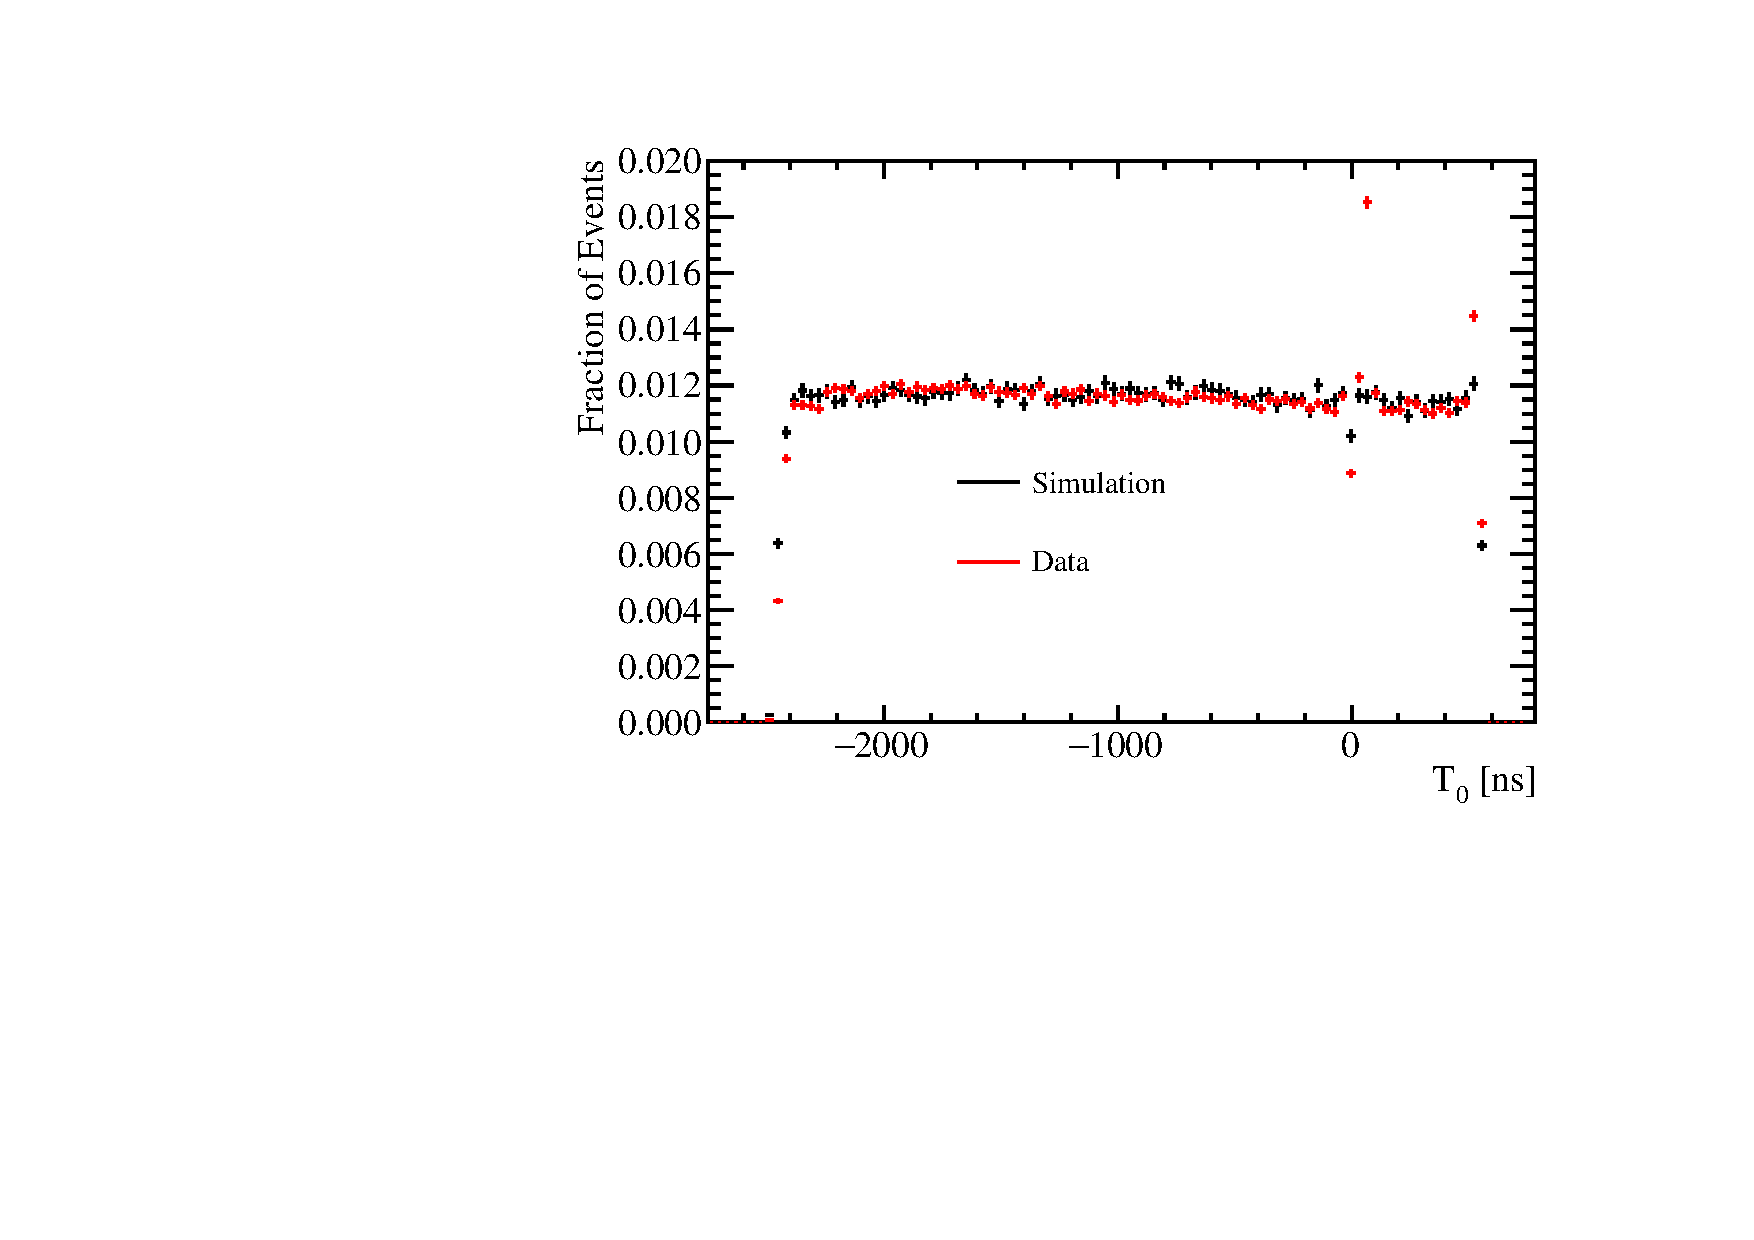
\includegraphics[width=1.0\textwidth]{Figures/Metrics/Data/Cosmics/StitchedT0.pdf}
\caption{The reconstructed $T_{0}$ distribution for data and MC.}
\label{fig:recoT0data}
\end{figure}

\section{Conclusions}

A summary of Pandora, a LArTPC pattern recognition software package, has been presented alongside relevant modifications allowing it to be applied to ProtoDUNE-SP.  The performance of Pandora has been extensively evaluated for simulation of the ProtoDUNE-SP detector.  Similarly, several pattern recognition metrics have been created and evaluated enabling a data MC comparison to be applied.  While differences are present, there is a generally good agreement between the two.  

The evaluation of the performance of Pandora for ProtoDUNE-SP is an important stepping stone in developing pattern recognition for the DUNE far detector.  The efficiencies quoted here must not be too readily extrapolated to the far detector.  Neutrino interactions in the far detector will be significantly easier to reconstruct in comparison to ProtoDUNE-SP because, unlike the underground far detector, ProtoDUNE-SP is a surface detector resulting in extensive cosmic ray backgrounds.  The peak of the momentum distribution is  similar to what is expected from primary particles produced from neutrino interactions, therefore, the successful reconstruction of test beam particles is extremely encouraging for preparing a reconstruction for the DUNE far detector.  Additionally over the coming years developments to the pattern recognition are to be expected from the development of new algorithms and the incorporation of deep learning techniques.  

\begin{acknowledgements}
This material is based upon work supported by the following: The European Union’s Horizon 2020 Research and Innovation programme under grant agreement No. 776262.
\end{acknowledgements}

% BibTeX users please use one of
%\bibliographystyle{spbasic}      % basic style, author-year citations
%\bibliographystyle{spmpsci}      % mathematics and physical sciences
%\bibliographystyle{spphys}       % APS-like style for physics
%\bibliography{}   % name your BibTeX data base

% Non-BibTeX users please use
\begin{thebibliography}{}
%
% and use \bibitem to create references. Consult the Instructions
% for authors for reference list style.
%
\bibitem{pandorasdk}
Marshall, J. S. and Thomson, M. A., The Pandora Software Development Kit for Pattern Recognition, Eur. Phys. J., C75, 439 (2015)
\bibitem{pandorauboone}
Acciarri, R. and others, The Pandora multi-algorithm approach to automated pattern recognition of cosmic-ray muon and neutrino events in the MicroBooNE detector, Eur. Phys. J., C78, 82 (2018)
\bibitem{pdtdr}
Abi, B. and others [DUNE Collaboration], arXiv:1706.07081 [physics.ins-det]
%\bibitem{RefJ}
% Format for Journal Reference
%Author, Article title, Journal, Volume, page numbers (year)
% Format for books
%\bibitem{RefB}
%Author, Book title, page numbers. Publisher, place (year)
% etc
\end{thebibliography}

\end{document}
% end of file template.tex

